%% Template for Master thesis
%% ===========================
%%
%% You need at least KomaScript v3.0.0,
%% e.g. available in Texlive 2009
\documentclass  [
  paper    = a4,
  BCOR     = 10mm,
  twoside,
  fontsize = 12pt,
  fleqn,
  toc      = bibnumbered,
  toc      = listofnumbered,
  numbers  = noendperiod,
  headings = normal,
  listof   = leveldown,
  version  = 3.03
]                                       {scrreprt}

% used pagages
\usepackage     [utf8]                  {inputenc}
\usepackage     [T1]                    {fontenc}
\usepackage                             {color}
\usepackage                             {amsmath}
\usepackage                             {graphicx}
\usepackage								{epsfig}
\usepackage     [english]               {babel}
\usepackage[square,numbers]{natbib}                             
\usepackage                             {hyperref}
\usepackage								{amssymb}
%\usepackage{BibLatex}
% links
\definecolor{darkblue}{rgb}{0.0,0.0,0.4}
\definecolor{darkgreen}{rgb}{0.0,0.4,0.0}
\hypersetup{
    colorlinks,
    linkcolor=black,
    citecolor=darkgreen,
    urlcolor=darkblue
}

\DeclareMathOperator*{\argmax}{argmax}

\begin{document}
  %% title pages similar to providet template instead of maketitle
  %% Titelseiten ähnlich zum Layout des Formulars von der
%% Fakultät für Physik und Astronomie
%%
%% Weitere Infos:
%% http://www.physik.uni-heidelberg.de/aktuelles/studium/
%% (PDF link: ...studium/download/145/Vorlage_Diplomarbeit_Formular.pdf)

%% Titelintro
\thispagestyle{empty}
\begin{center}
  \renewcommand{\baselinestretch}{2.00}
  \Large\sffamily
  Fakult\"{a}t f\"{u}r Physik und Astronomie\\
  \large
  Ruprecht-Karls-Universit\"{a}t Heidelberg
  \par\vfill\normalfont
  Masterarbeit\\
  Im Studiengang Physik\\
  vorgelegt von\\
  (Vor- und Zuname)\\
  geboren in (Geburtsort)\\
  (Jahr der Abgabe)\\
\end{center}
\newpage

%% Titelseite
\thispagestyle{empty}
\begin{center}
  \renewcommand{\baselinestretch}{2.00}
  \Large\bfseries\sffamily
    (Titel)\\
    (der)\\
    (Masterarbeit)
  \par
  \vfill
  \large\normalfont
  Die Masterarbeit wurde von (Vorname Name)\\
  ausgef\"{u}hrt am\\
  (Institut)\\
  unter der Betreuung von\\
  (Frau/Herrn Prof./Priv.-Doz. Vorname Name)
  %% Bei externen Masterarbeiten hier noch den zweiten Betreuer einfügen
  %% und den vspace in Z. 45 entsprechend reduzieren
\end{center}\par
\vspace{5\baselineskip}

% Zeilenabstand zurücksetzen
\renewcommand{\baselinestretch}{1.00}\normalsize % select either german
  %% this will generate title pages similar to the template provided
%% by the Department of Physics and Astronomy Heidelberg
%%
%% More information:
%% http://www.physik.uni-heidelberg.de/aktuelles/studium/
%% (PDF link: ...studium/download/145/Vorlage_Diplomarbeit_Formular.pdf)

%% Titleintro
\thispagestyle{empty}
\begin{center}
  \renewcommand{\baselinestretch}{2.00}
  \Large\sffamily
  Department of Physics and Astronomy\\
  \large University of Heidelberg
  \par\vfill\normalfont
  Master thesis\\
  in Physics\\
  submitted by\\
  Jacob Nieswand\\
  born in Konstanz\\
  2018
\end{center}
\newpage

%% Titlepage
\thispagestyle{empty}
\begin{center}
  \renewcommand{\baselinestretch}{2.00}
  \Large\bfseries\sffamily
    Optimizations of Light Field measurements\\
    using the structure tensor
  \par
  \vfill
  \large\normalfont
  This Master thesis has been carried out by Jacob Nieswand\\
  at the\\
  Institut für wissenschaftliches Rechnen (IWR)\\
  under the supervision of\\
  Herrn Priv.-Doz. Christoph Garbe
  %% additionally insert second supervisor here if carrying out an
  %% external diploma thesis. Reduce vspace in L. 44 accordingly.
\end{center}\par
\vspace{5\baselineskip}

% reset baselinestretch
\renewcommand{\baselinestretch}{1.00}\normalsize % or english title page
  %% Abstract page
%% =============
%%
%% Content of abstract pages has been put into seperate pages to simplify
%% word counting. Use e.g. the unix command
%%   wc abstract-ger.tex
%% or
%%   wc abstract-eng.tex
%% to get the number of words contained in these files.
\thispagestyle{empty}
\begin{center}
  \begin{minipage}[c][0.48\textheight][b]{0.9\textwidth}
    \small
    \textbf{
      Optimierung von EPI-basierten Lichtfeldmessungen:
    }\par
    \vspace{\baselineskip}
    
Diese Arbeit befasst sich mit der Tiefenrekonstruktion einer Szene mittels 2D-Aufnahmen aus verschiedenen Blickwinkeln (Lichtfeld). Aus der Struktur der epipolaren Schnitte durch das Lichtfeld (EPIs) wird mithilfe des Strukturtensors die Tiefe errechnet. In dieser Arbeit werden verschiedene Modifikationen bestehender entwickelter Algorithmen getestet, weiterhin werden Depth-of-defocus- Techniken getestet und verglichen. Zusätzlich wird ein Algorithmus basierend auf dem in der Stereo-Vision verbreiteten Semi-global Matching Algorithmus (SGM) als Nachbearbeitungsschritt implementiert.
  \end{minipage}\par
  \vfill
  \begin{minipage}[c][0.48\textheight][b]{0.9\textwidth}
    \small
    \textbf{
      (Title of Master thesis - english):
    }\par
    \vspace{\baselineskip}
    This work deas with 3D depth reconstruction of a scene using 2D images captured from different angles (light field imaging). From the structure of the Epipolar Plane Images (EPIs) the depth is calculated using the structure tensor In this thesis various modifications of existing algorithms will be developed and tested, further depth-of-defocus techniques will be tested and compared. In addition, an algorithm based on the SemiGlobal Matching Algorithm (SGM) ,commonly used in Stereo vision, is implemented as a postprocessing step.
  \end{minipage}
\end{center}


  \tableofcontents
  %% Put your contents here

\bibliographystyle{abbrvnat}
\setcitestyle{authoryear}
\chapter{Introduction}
In the field of computer vision, one big challenge is the 3D reconstruction based on 2D images. When reconstructing the depth based on two images capturing the scene from two points in space, we speak of \textit{stereo vision}. If a specific feature point in one image can be detected in the other image as well, the distance of the feature point to the cameras can be calculated via triangulation.\\
The necessity for depth imaging is reasoned by the sheer amount of different applications, reaching from industrial quality management to the creation of CGI effects as well as applications in the gaming industry. 3D reconstruction recently has become irreplaceable in the car industry related to the development of autonomous driving systems. Another industrial application is the robotic vision for improving automation setups, such as vision-controlled pick-and-place systems.\\

Obtaining 3D Information via a camera system is mainly done by using either stereo camera systems, structured light systems, TOF(Time-of-flight)-cameras or interferometry cameras. While the last 3 mentioned systems are capable of reconstructing 3D-scenes of diffuse surfaces quite well, they do not make use of the surface RGB values.\\
Recently \textit{light field imaging} as an expansion of stereo imaging has become a main field of research in computer vision. By capturing the scene from multiple viewpoints, a whole bunch of data can be processed to not only reconstruct the depth more robustly but also enable making statements about the surface characteristics. The real-time processing of a sufficient amount of 2D data still remains a challenge. \\
Further, reconstructing the 3D image from 2D images comes with challenging tasks:
\begin{itemize}
	\item Occlusions: As we cannot see the full scene from each viewpoint, some points of the surface we are looking at are either partly or fully occluded.
	\item Single-coloured surfaces: Parts of the scene with low textural structure make viewpoint-to-viewpoint-matching barely possible.
	\item Glossy surfaces: When developing a 3D reconstruction solution based on the assumption of \textit{Lambertian} surfaces, we assume a surface point to be in the same colour no matter from which position/angle we look at it. However, this is not the case for reflective/glossy surfaces.
\end{itemize}
In this work, we try to tackle those problems using a depth reconstruction algorithm based on the work of \cite{wanner2014orientation} while maintaining reasonable calculation times.\\
Advanced research on light field depth reconstruction has been published by \cite{diebold2016light}, expanding the approach to heterogeneous light fields. \cite{schoenpflug2017optimizing} conducts research at inpainting low-feature areas in light field depth maps. In the work of \cite{freist2018reconst}, modifications on the algorithm of Wanner as well as a graph-based post-processing optimization method are proposed for obtaining improved depth maps.\\
\chapter{Theory}\label{chapter_theory}
\section{Light field parametrization}
The earliest introduction to light fields in literature can be found in \cite{adelson1991plenoptic}, where they parametrize the field of light as a  so-called 'plenoptic function'. If we assume that every point in space emits a light ray  in a given direction which is characterized by an intensity value $P$, the whole information in the light field is given as a 6-dimensional function
\begin{equation}\label{key}
P(V_x,V_y, V_z, \theta, \phi, \lambda),
\end{equation}
where $\theta$ and $\phi$ are the solid angles describing the direction of any light field, $\lambda$ describes the wavelength dependence. $V_{\{x,y,z\}}$ describe the room coordinates. If we use the pixels of a pinhole camera image as the coordinate system of our choice, the plenoptic function would be parametrized as 
\begin{equation}\label{eq:plenoptic}
P(x,y, V_x, V_y, V_z, \lambda).
\end{equation}
 A more generalized model of the plenoptic function could also include a time dependence, leading to a 7-dimensional ray space. In general, the plenoptic function serves as the global function that gets mapped into a low-dimensional space in some form by any camera device, e.g. a pinhole camera mapping the whole ray space down to a 2-dimensional image.\\
\setcitestyle{numbers}
 	
 A more detailed introduction to light fields can also be found in \cite{wanner2014orientation}. 
\setcitestyle{authoryear}
\subsection{The Lumigraph}
In the form of equation \ref{eq:plenoptic} the plenoptic function is a 7-dimensional function, which is difficult to record and to handle. As described by \cite{wu2017light} this plenoptic function is usually simplified in 3 steps: First, we neglect the time dependence assuming a static scene. Further, we neglect the wavelength $\lambda$. Instead, we define the mapped value of the plenoptic function as a vector containing the colour channels. 
Additionally, the plenoptic function obtains redundant information because light rays, lying on one line in space, propagate in the same direction, as introduced by \cite{bolles1987epipolar}. The 4D-representation is also known as the \textit{Lumigraph}. Those 4 dimensions can be split to 2 angular dimensions describing the direction of each ray and 2 dimensions for the location of the ray: Since every ray would pass an image plane of infinite size once (if the propagation vector is not parallel), two coordinates for localizing the ray are sufficient. Commonly the \textit{two-plane-parametrisation} is used to describe the light field. Every ray is characterized by the intersection of two arbitrary parallel planes $\Pi$ and $\Omega$. Mathematically spoken the light field $L$ is a function
\begin{equation}\label{key}
L:\Omega\times \Pi \rightarrow \!R\qquad x,y,s,t\rightarrow L(x,y,s,t),
\end{equation}
where $x,y$ are the coordinates in the first plane $\Omega$ and $s,t$ are the coordinates in the second plane $\Pi$. If we move a camera in a plane and take pictures of a scene orthogonal to the camera plane, the image itself is described by the image coordinates $x,y$ while the position of the camera is denoted as $s,t$. Both planes are parallel to each other; that way a light field can be measured in a straightforward manner.
\setcitestyle{numbers}
\begin{figure}[h!]
	\centering
	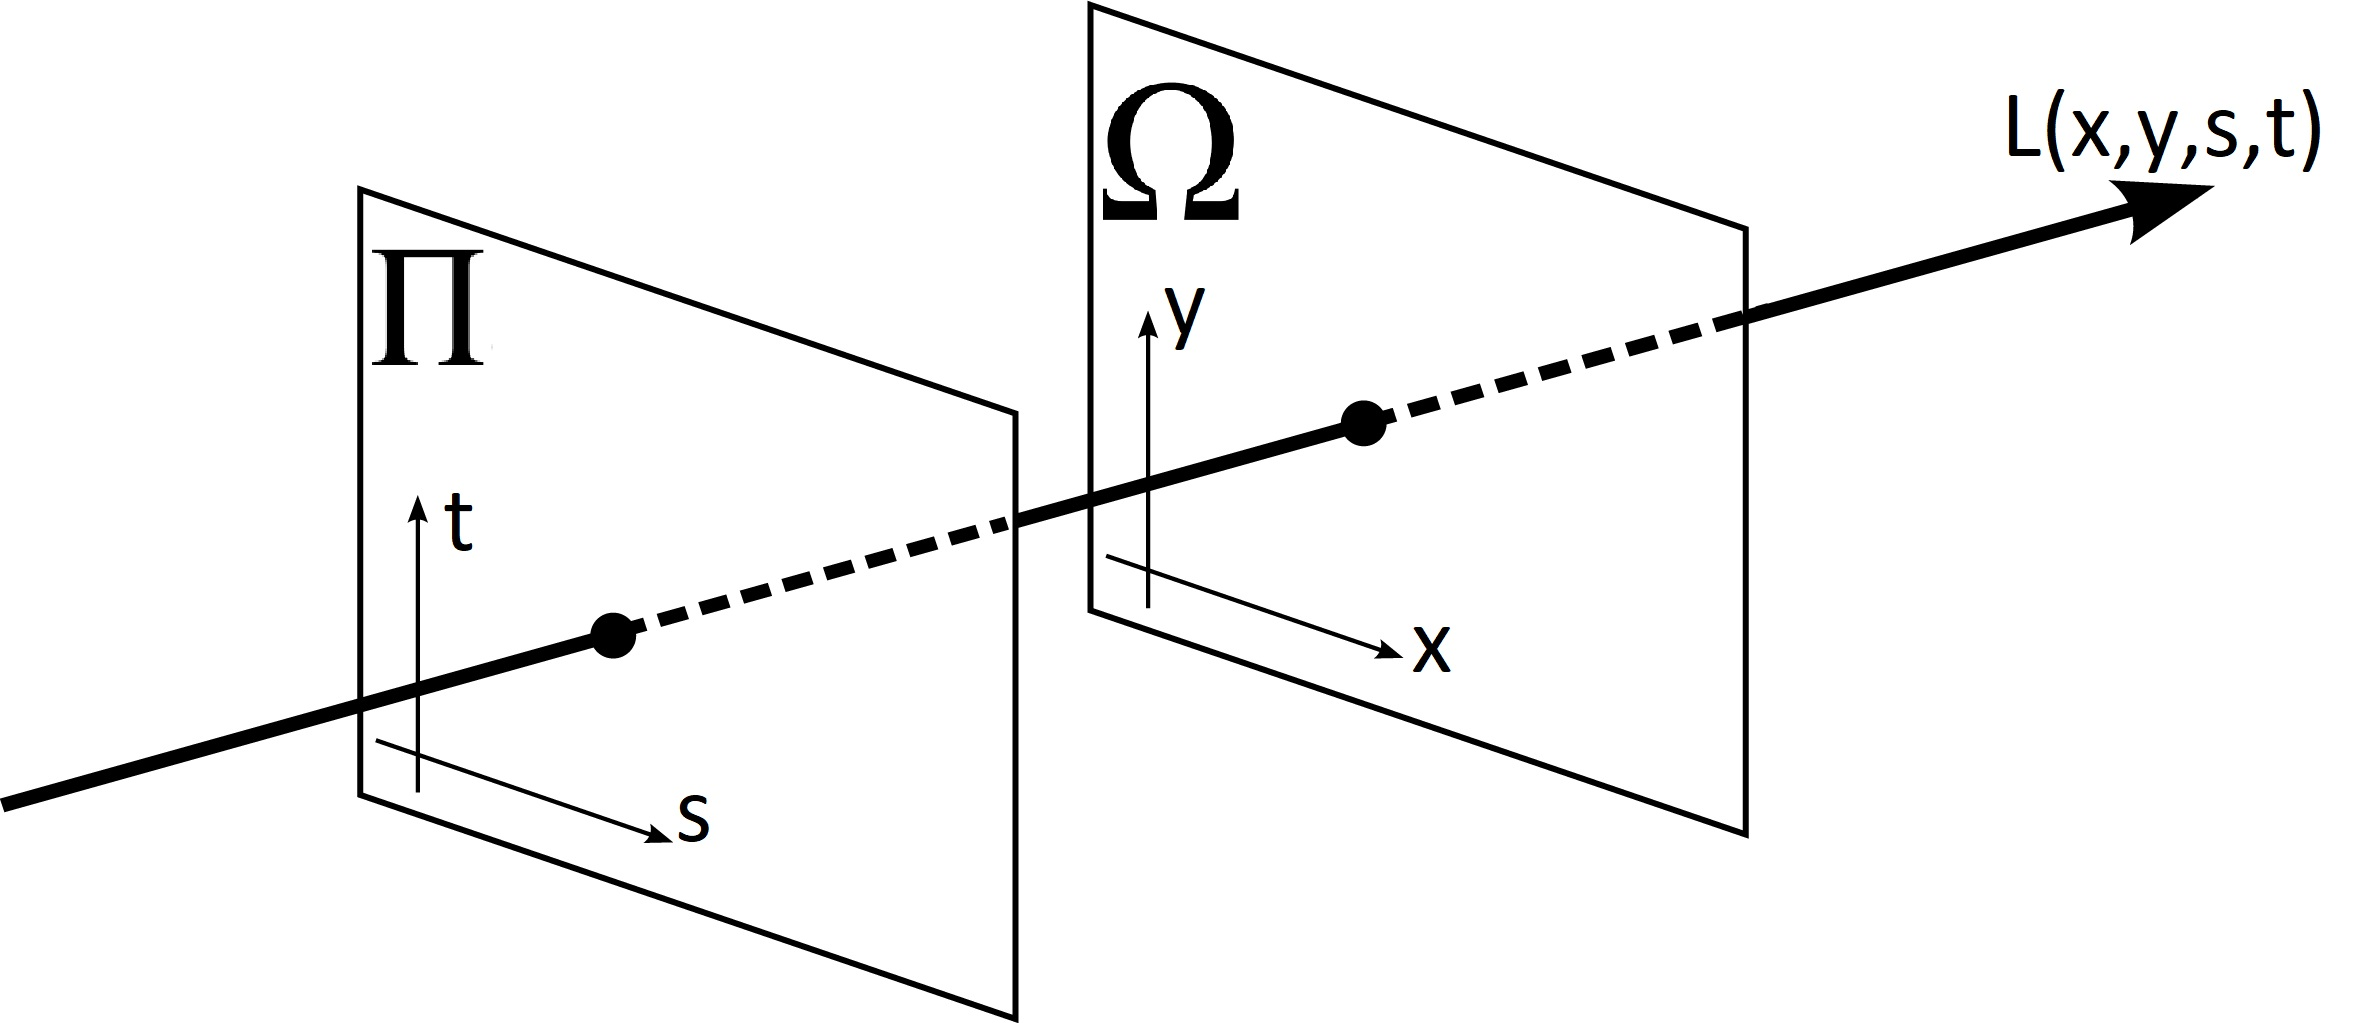
\includegraphics[width=0.7\linewidth]{images/twoplane_param}
	\caption[Two-plane parametrisation]{In a 4-dimensional two-plane parametrisation a light ray is characterized by the intersection with two parallel planes. We refer to the plane  $\Pi$ as the camera plane and the plane $\Omega$ as the image plane. From \cite{Xu:12}}
	\label{fig:twoplaneparam}
\end{figure}
\setcitestyle{authoryear}
\subsection{Epipolar plane images}
\label{sec:epi}
\begin{figure}[h!]
	\centering
	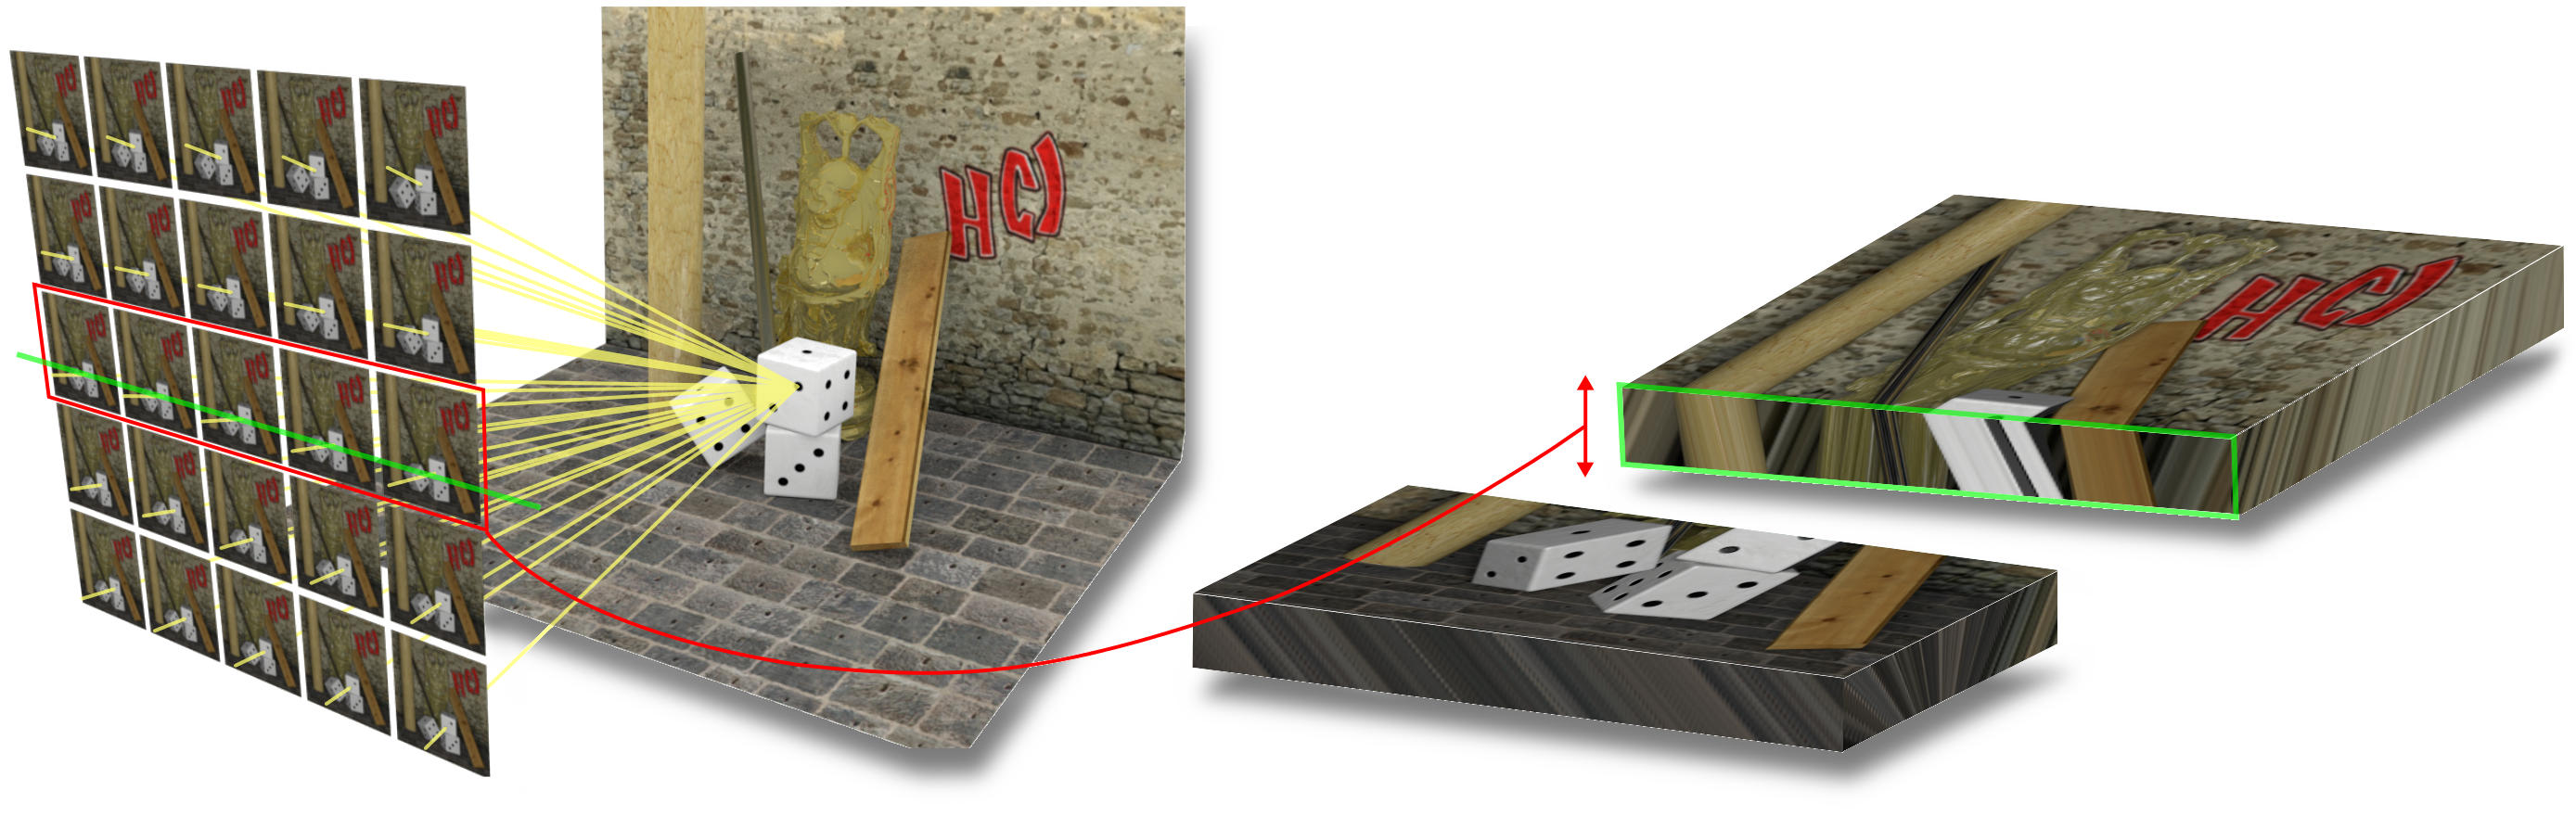
\includegraphics[width=1\linewidth]{images/epiVisualization}
	\caption[Visualization of an EPI extraction]{Visualization of an epipolar plane image extraction: A camera array takes images of the same scene from slightly different angles (left array). For a fixed image coordinate $y^*$ (green) and a fixed camera coordinate $t^*$ (red) the pixels are extracted and stacked up resulting in an EPI $\Sigma_{y^*, t^*}$ (green box on the right). From\setcitestyle{numbers}\cite{iwr.uni-heidelberg.de}\setcitestyle{authoryear}}
	\label{fig:epivisualization}
\end{figure}
We measure the light field in order to obtain as much information about the scene we are looking at as possible. In order to obtain the 3-dimensional structure one needs to map the light field in a certain manner: We take a look at one 2-dimensional slice through the 4-dimensional space while keeping 2 coordinates constant: one horizontal coordinate  $x^{*}$  in the image plane and one vertical coordinate $t^{*}$ in the camera plane (or vice versa). The slice $\Sigma_{x^{*}, t^{*}}$ is a 2-dimensional image called \textit{epipolar plane image} (EPI). In figure \ref{fig:epivisualization} the extraction of an EPI from camera array data is visualized. As seen in figure \ref{fig:simpleepi} it consists of lines with different slopes, each point on one line with the same slope belongs to the same point in the scene viewed from different angles. From the slope $\Delta$ we obtain the distance from the camera plane with the equation
\begin{equation}\label{eq:distance}
\text{distance} = \frac{f\cdot b}{\Delta},
\end{equation}
where $f$ is the focal length of the camera and $b$ is the baseline between the camera positions. One may notice that this equation looks equal to distance estimation in stereo vision, where we replace the slope $\Delta$ by the disparity shift of a feature in 2 views. In fact, a stereo light field capture would result in an EPI with only two pixel rows, the slope of a line consisting of only two points is then defined as the disparity shift between the views.
\begin{figure}[h!]
	\centering
	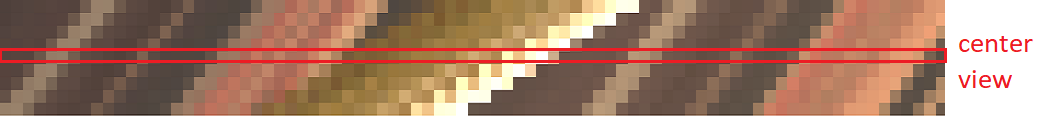
\includegraphics[width=1\linewidth]{images/simple_epi}
	\caption[Example epipolar plane image]{An epipolar plane image (EPI) that consists of 9 rows (9 equidistant views or sample points in the camera plane). Points with the same colour correspond to the same scene point. Since the viewpoints are slightly shifted, the scene point is also shifted in each view by the disparity $d$. The pixels from the centre view position are marked in red.}
	\label{fig:simpleepi}
\end{figure}


\section{Depth from structure tensor}
Measuring depth from light field data can be done using various approaches.
\cite{wu2017light} divide light field depth estimation approaches in three categories:
\begin{enumerate}
	\item Sub-aperture image matching-based methods
	\item EPI-based methods
	\item Learning-based methods
\end{enumerate}
In the following, we focus on one specific EPI-based method on which is investigated as part of this work. However, the reader is encouraged to take a look at the cited publication 'Light Field Image Processing: An Overview' by \cite{wu2017light} for a state-of-the-art overview of different light field approaches.\\
\cite{wanner2014orientation} makes use of the oriented structure of the EPI using image-processing techniques. This idea has first been introduced by \cite{bigun1987optimal} in 1987.\\

The 2-dimensional structure tensor $J$  on a function $g:\Omega \rightarrow \!R, \Omega \subset \!R^2 $ is defined as
\begin{equation}\label{eq:structuretensor}
J =\left(
\begin{matrix}
G*\frac{\partial g}{\partial x}\frac{\partial g}{\partial x} & G*\frac{\partial g}{\partial x}\frac{\partial g}{\partial s} \\
G*\frac{\partial g}{\partial s}\frac{\partial g}{\partial x} & G*\frac{\partial g}{\partial s}\frac{\partial g}{\partial s} 
\end{matrix}\right),
\end{equation}
 where $G$ is a Gaussian window function. The derivation can be found in the appendix.
 The first eigenvector of this tensor $J$ indicates the preferred orientation in the local neighbourhood (defined by the window function). The second eigenvector is orthogonal to the first. 
 
   \cite{jahne2013digitale} proposes a coherence value as a measurement for the anisotropy of the local environment:
 \begin{equation}\label{eq:coherence}
 C = \frac{\sqrt{(J_{11} - J_{22})^2 + 4J_{12}^2}}{J_{11} + J_{22}}
 \end{equation}
 which obeys the value 1 in case of complete anisotropy, a value of 0 would indicate total isotropy.\\
 In case of an EPI, the structure tensor provides an estimate for the slope of an EPI line, as defined by \cite{bigun1987optimal}:
 \begin{equation}\label{eq:disparity}
 \Delta = \tan\left(\frac{1}{2} \arctan\left( \frac{J_{22}-J_{11}}{2J_{12}}\right)\right)
 \end{equation}
 we refer to $\Delta$ as the disparity $d$ in the following. Via equation \ref{eq:distance} one obtains the depth in meters.
 
 \subsection{Implementation}
 The following implementation steps have been proposed by \cite{wanner2014orientation}. The code uses \textit{crosshair} light field data that can be obtained e.g. by a camera as depicted in figure \ref{fig:lumiplus}. Instead of a full 2D camera array, the scope of the light field in the camera coordinates is significantly reduced. In the following, the horizontal camera row and the vertical camera column are viewed separately as 1-dimensional light-field cameras.\\
 \begin{figure}[h!]
 	\centering
 	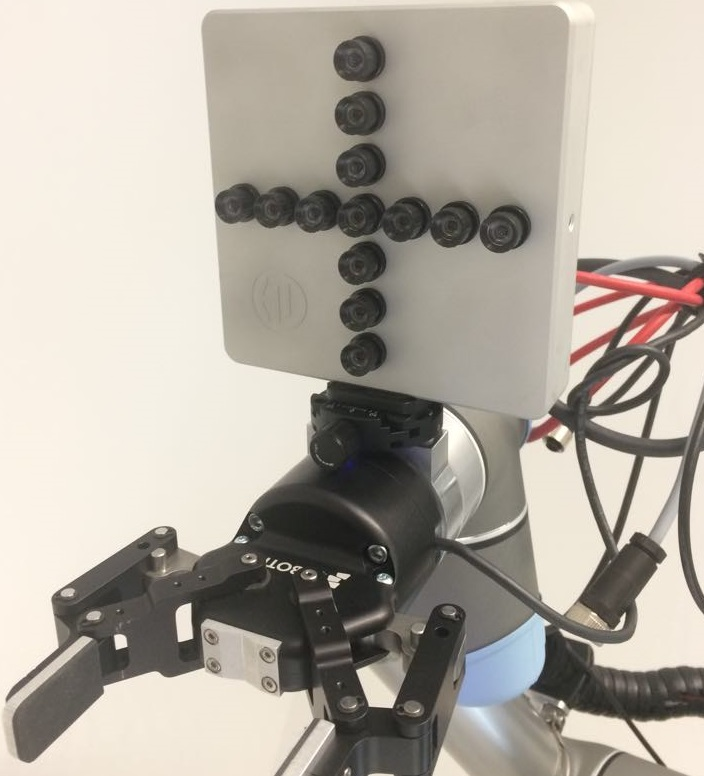
\includegraphics[width=0.5\linewidth]{images/Lumiplus}
 	\caption[LumiPlus Scanner from HDVision Systems]{Instead of a complete camera array a crosshair camera reduces the number of cameras to one row and one column for faster processing. This \textit{Lumi+} - Scanner from HDVision Systems is mounted on a robot arm for industrial applications.}
 	\label{fig:lumiplus}
 \end{figure}
 
 From the input images one extracts the EPIs, which have the dimensions
 \begin{align*}
 \text{vertical view}&\rightarrowtail \text{Nr of rows in image coordinates }\times \text{Nr of cameras}\\
 \text{horizontal view}&\rightarrowtail \text{Nr of columns in image coordinates }\times \text{Nr of cameras}
 \end{align*}
 
 For each EPI we calculate the structure tensor independently. This is done by first pre-smoothing the EPI with a $3\times3$ Gaussian kernel to avoid noise. Note that before calculating the gradient, the EPI is converted to grey-scale format.\\
 The gradient is calculated via the Scharr-filter, which has the form
 \begin{align}\label{key}
 \text{Scharr}_x &= \left(\begin{matrix}
 3&0&-3\\
 10&0&-10\\
 3&0&-3
 \end{matrix}\right)
\\
 \text{Scharr}_y &= \left(\begin{matrix}
 3&10&3\\
 0&0&0\\
 -3&-10&-3
 \end{matrix}\right).
 \end{align}
 \cite{wanner2014orientation} and \cite{diebold2016light} both tested out different gradient filters and came to the conclusion that the Scharr-filter performs best. With the gradients the structure tensor and the disparity is obtained via equation \ref{eq:structuretensor} and \ref{eq:disparity}.\\
 Further, Wanner found out that the structure tensor results are most accurate when the disparity is close to zero. Therefore the EPI is artificially refocussed by a simple linear shifting of the rows such that the slope of any line in the EPI would be increased by the same amount. The disparity shift can simply be subtracted from the disparity later. The refocussing of the EPI is illustrated in \ref{fig:refocusedcut}. For each EPI the structure tensor is calculated at each disparity shift so that the necessary disparity range is fully covered.  \\
The value with the highest coherence measure (equation \ref{eq:coherence}) is selected from all disparity shifts. Hence one obtains two depth estimations for each image coordinate in the centre view: one from the vertical EPI, one from the horizontal EPI. The merging of both direction follows
 \begin{equation}\label{key}
 d(x,y) = \begin{cases} d_\text{horizontal}(x,y) & C_\text{horizontal}(x,y)>C_\text{vertical}(x,y)\\
 						d_\text{vertical}(x,y) & C_\text{horizontal}(x,y)<C_\text{vertical}(x,y)\\
 		\end{cases}.
 \end{equation} 
 This implementation is referred to as the structure tensor (ST) pipeline in the following.
  \begin{figure}[h!]
 	\centering
 	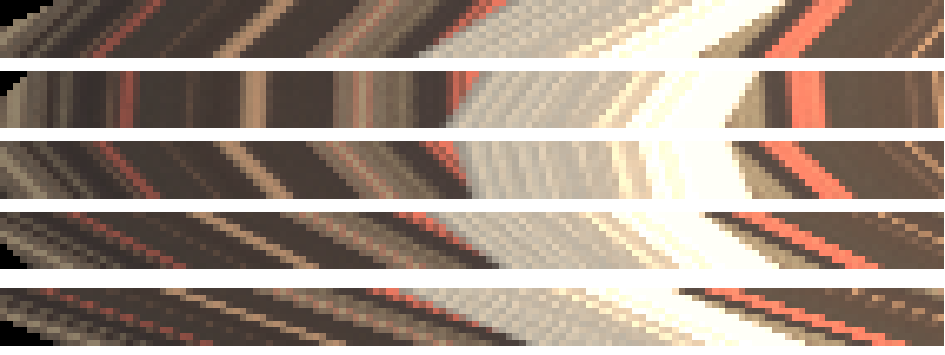
\includegraphics[width=0.7\linewidth]{images/refocused_cut}
 	\caption[Refocussed EPI]{The EPI is refocussed by integer disparity steps. If the slope at a scene point is zero (vertical line) the EPI is perfectly focussed on that point. An integration of all views would still result in a sharp image at the corresponding depth.}
 	\label{fig:refocusedcut}
 \end{figure}
 \subsection{The occlusion problem of the structure tensor}
 \label{sec:occlusionproblem}
 Having a look at the results of the benchmark test of \cite{honauer2016benchmark}, one realizes that most light field depth estimation algorithms suffer from large errors near depth discontinuities. Since the angular pixels close to the edge of a depth discontinuity are at least partly occluded, a loss of accuracy near discontinuities is expected. The ST almost always produces a systematic error near discontinuities, leading to a 'magnification' of the object closer to the camera in the depth map, see figure \ref{fig:cottondiscontinuities0070}. We refer to this as 'edge fattening'. The reason for this error has its origin in the smoothing of the EPI as part of the algorithm.  At the occlusion, the edge between the fore- and background follows the same orientation as the foreground does. \\
  Furthermore, the occlusion mostly comes with a colour change, resulting in a high gradient which dominates the local environment orientation: Edge fattening is the consequence. In figure \ref{fig:occlusion} one can recognize two effects leading to edge fattening: Firstly the EPI is smoothed with a $3\times 3$ Gaussian kernel which already will enlarge the foreground structure (b). This becomes clear when we illustrate the norm of the gradients (c), since the strong (white) gradients all measure the foreground (green) structure. A clear shift to the left is visible from (b) to (c). However, this bias error is small compared to the second error that is indicated in (d): The red dot lies clearly in the background structure. Calculating the structure tensor components from the local environment (green square), one would obtain the foreground structure at the red dot, since the strong gradients in the square dominate. In (e) the total bias in labelling the two structures is illustrated. 
  \begin{figure}[h!]
  	\centering
  	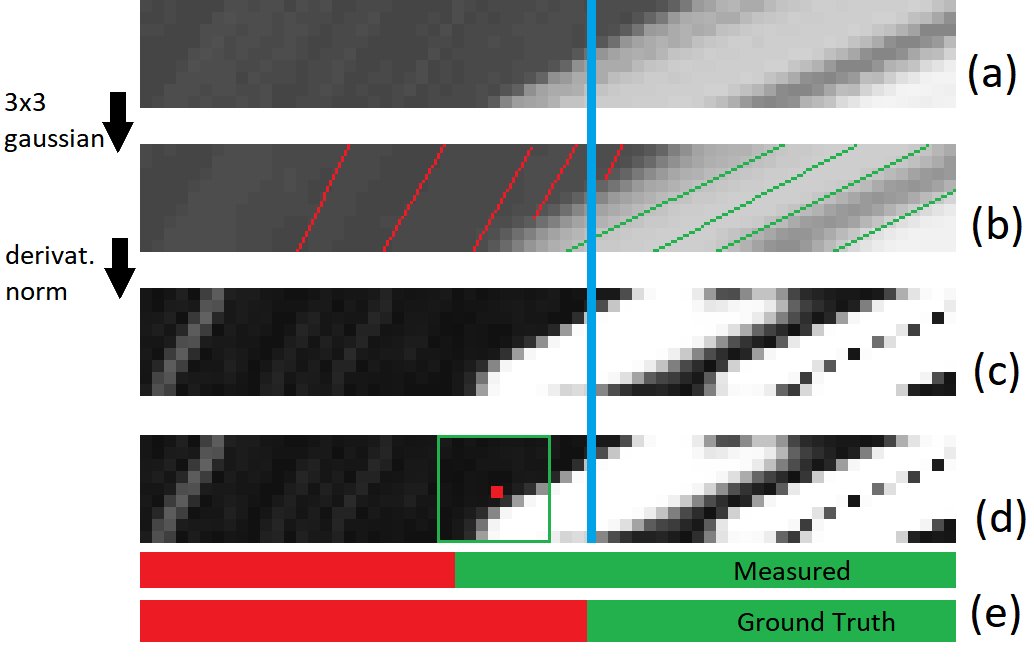
\includegraphics[width=0.7\linewidth]{images/occlusion_painted2}
  	\caption[Occlusion in an EPI]{(a) The structure of an occlusion border in a grey-value EPI. (b) Before calculating the gradient, the EPI is smoothed with a $3 \times 3$ Gaussian kernel. One sees the smoothed EPI with coloured lines indicating the Ground Truth orientation. (c) shows the norm of the gradient calculated via the Scharr-filter. White represents a high gradient, black represents a low gradient. In (d) the local environment around the red dot $(x_r,y_r)$ as an example point is marked to show which gradient values go into the structure tensor components $J(x_r,y_r)$. (e) marks the orientation labelling measured and ground truth. The blue line marks the transition in the centre view that corresponds with the ground truth labelling. }
  	\label{fig:occlusion}
  \end{figure}
\begin{figure}[h!]
	\centering
	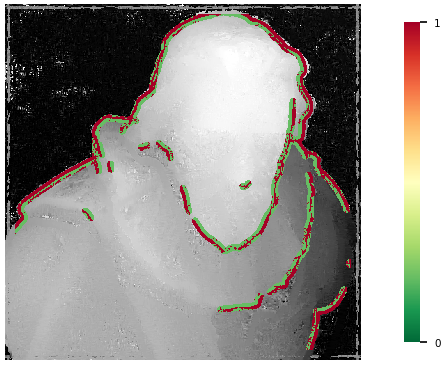
\includegraphics[width=0.7\linewidth]{images/cotton_discontinuities_0070}
	\caption[Discontinuity evaluation]{Evaluation of the deviation from ground truth at the depth discontinuity for scene \textit{cotton}. In red/green the mask for calculating the deviation is depicted. If the disparity deviation is greater than 0.07 pix, it is coloured red.}
	\label{fig:cottondiscontinuities0070}
\end{figure}
  
 \section{Modifications on the structure tensor}
 In the following, different methods will be explained which modify the structure tensor algorithm proposed by \cite{wanner2014orientation}. In section \ref{Evaluation} implementations of those modifications will be evaluated and discussed.
 \subsection{Kernel sizes}
 The structure tensor algorithm calculates the depth based on the preferred orientation of the EPI in a local neighbourhood. If one chooses a larger neighbourhood, the resulting depth map is likely to be smoother, while the accuracy at edges in the scene rapidly decreases.
 Even though one often wants to smoothen the depth map in a post-processing step to reduce the noise and cancel out outliers, the structure tensor algorithm by Wanner is forced to smoothen the depth map in the process by estimating the depth from the local neighbourhood in the EPI. In the work of \cite{wanner2014orientation} the effect of the kernel size has been examined extensively and he calculated the best parameters for different scenes by grid search. Note that if the kernel is smaller than the height of the EPI, the outer cameras are neglected and do not enter in the calculation of the depth. To maintain the information of all cameras and vary the kernel size at the same time, \cite{diebold2016light} proposes asymmetrical kernel sizes to eventually reduce edge-fattening effects. However, asymmetrical kernels still need to find a trade-off between denoising and avoiding edge fattening and do not significantly increase the quality of the depth map result.\\
 Another approach is to choose a custom kernel form which only weights the local gradients that could possibly be part of the 'correct' line in the EPI. Such a kernel is illustrated in figure \ref{fig:sandclock},  it has the form of a sandglass. In y-direction, it still follows a Gaussian distribution.
 \begin{figure}[h!]
 	\centering
 	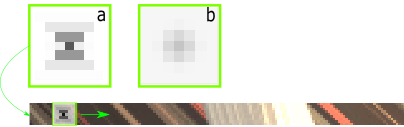
\includegraphics[width=0.7\linewidth]{images/sandclock.png}
 	\caption[Sandglass kernel]{(a) shows a custom-shaped kernel in form of a sandglass. (b) shows a normal Gaussian kernel. The kernels are used for the calculation of the ST components along the EPI.}
 	\label{fig:sandclock}
 \end{figure}
 \subsection{Colour-awareness with bilateral filtering}
 \label{sec:bilateral}
 In its original form the structure tensor pipeline weights the square of all gradients in a local environment by the distance to the reference point. Since all local gradients in the EPI that belong to the same colour are very likely to belong to the same orientation, one has to find all points with the same colour which then lie on the same line in the EPI in case of a Lambertian surface. The preferred orientation of the gradients at those points will then correspond to their slope with high confidence. However, most objects are not perfectly Lambertian such that not all points on the correct line have to be of the exact same colour. Only filtering the exact colour will lead to noisy results. Instead, one could implement a filter weighting not only the distance in a Gaussian manner but also the distance from the  EPI kernel origin in the colour RGB space; such a filter is called 'bilateral filter' (\cite{tomasi1998bilateral}). Pixels with completely different colour will be excluded from the neighbourhood when calculating the structure tensor. In equation \ref{eq:structuretensor} the window function $G$ is then defined as 
 \begin{equation}\label{eq:bilateral}
 G_P = \frac{1}{W_p}\sum_{q\in N} g_{\sigma_d}(||p-q||) g_{\sigma_c}(||I_{p, \text{EPI}}-I_{q, \text{EPI}}||),
 \end{equation}
 where
 \begin{itemize}
 	\item[$p$] is the position of the pixel,
 	\item[$q$] is the position of the pixel in a neighbourhood $N$,
 	\item[ $g_{\sigma_d}$] is a Gaussian function weighting the distance between $p$ and $q$ using $\sigma_d$ as standard deviation,
 	\item[ $g_{\sigma_c}$] is a Gaussian function weighting the colour distance in RGB space between the  RGB values of the original EPI at $p$ and $q$ using $\sigma_c$ as standard deviation,
 	\item[$W_P$] is a normalization factor so that the sum over all the neighbourhood always is 1. 
 \end{itemize}


It is important to notice that the colour distance is extracted from the EPI, though we are filtering the components of the second derivatives, see equation \ref{eq:structuretensor}. In fact, the EPI only serves as a guide for the filtering.
 \subsection{Thresholding the gradients}
 \label{sec:thresholdinggradients}
 In section \ref{sec:occlusionproblem} it is explained why the structure tensor struggles to serve with a  good estimation at depth transitions. It is referred to two errors; one coming from the first smoothing, the other one as a result from the second Gaussian smoothing. To avoid the second error, one could in principle normalize all local gradients such that in figure \ref{fig:occlusion} (d) the foreground gradients in a local environment obey the same weight in the structure tensor calculation as the background gradients around the red dot.\\
 The gradient components of the EPI would be given by
 \begin{align}
 	\tilde{\vec \nabla}(x,y) = \frac{1}{\sqrt{\nabla_x(x,y)^2 + \nabla_y(x,y)^2}} \vec \nabla_x(x,y)
 \end{align}
 Nevertheless, on some occasions one wants the stronger gradients to play a bigger role in the preferred orientation since small gradients are more likely to be noisy. One way to damp the gradients at occlusions while not strengthening the small noisy gradients in an EPI is to implement a \textit{truncation threshold}. The gradient is then given by
 \begin{align}
 \tilde{\vec \nabla}(x,y) &= \begin{cases}
\frac{\text{threshold}}{\text{norm}} \vec \nabla(x,y) \quad &\text{if}\quad \text{norm}> \text{threshold}\\
\tilde{\vec \nabla}(x,y)\qquad &\text{else}\\
 \end{cases} \\
\text{with} \quad \text{norm} &= \sqrt{\nabla_x(x,y)^2 + \nabla_y(x,y)^2}.\\
 \end{align}
 The threshold should be chosen the lowest possible in a manner that gradients higher than the threshold are barely affected by noise. In section \ref{sec:ev_thresh} different thresholds are tested, if not mentioned otherwise a threshold of 0.1 is used assuming that the underlying EPI is a grey-value image with range 0-1.\\
 
 \subsection{Occlusion-awareness using segmentation of the EPI}
 \label{sec:occlusionsegmentation}
 \begin{figure}[h!]
 	\centering
 	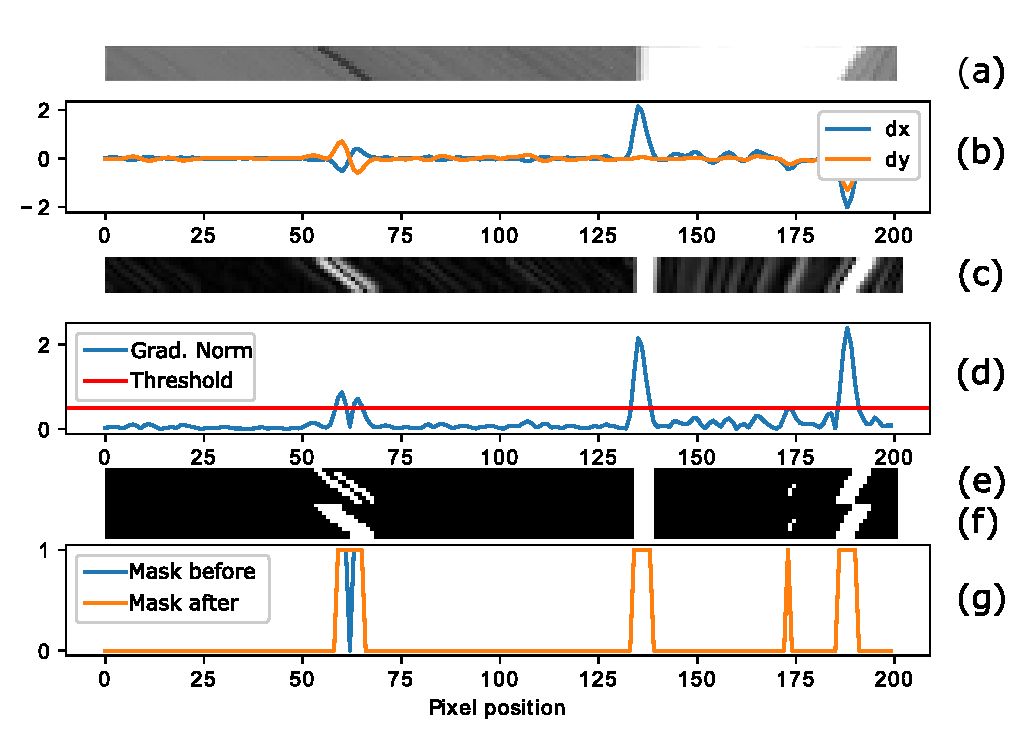
\includegraphics[width=1\linewidth]{images/derivatives_full}
 	\caption[Segmenting an EPI]{(a) Input EPI to be segmented. (b) shows the local derivatives along the centre view line. (c) shows the vector norm of the derivative. (d) shows the centre view norm with the threshold that is applied to mask transitions. (e) shows the resulting mask. (f) shows the improved mask using morphological image processing. (g) shows the centre view line from (e,f). }
 	\label{fig:derivativesfull}
 \end{figure}
 In this section, a method is proposed that attempts to handle both occlusion errors mentioned in section \ref{sec:occlusionproblem}.\\
 Bilateral filtering (section \ref{sec:bilateral}) and thresholding the gradients (section \ref{sec:thresholdinggradients}) may improve the depth map estimation, however they come with trade-offs in order to handle the occlusion problems. An alternative way to maintain sharp transitions is to find those transitions in the EPI and calculate them separately. By setting the gradient at the transition in the EPI to 0, background and foreground structure are calculated without being biased by the gradient of the transition itself. Therefore the EPI is segmented binarily into occlusion transitions and continuous areas, whereby the norm vector is thresholded to create a binary mask on the EPI. \\
 Possibly one could think of a better criterion for segmenting occlusion/non-occlusion areas than the norm vector size. However, using this binary mask there is no need to calculate the disparity values beforehand and it can be implemented in the workflow directly. In principle the algorithm works as follows:
 \begin{enumerate}
 	\item Segment the transitions and the rest of the EPI with a binary mask based on the gradient norm.
 	\item Calculate the structure tensor components on the masked gradient of the EPI. All masked gradients are zero and do not affect the local environment structure.
 	\item Calculate the structure tensor components again, now on the inverted masked gradient of the EPI.
 	\item Join the disparity values from both masks.
 \end{enumerate}
 In figure \ref{fig:derivativesfull} the segmentation process is illustrated step-by-step. The gradient of the grey-value EPI (a) is calculated in x- and y-direction (b), from which one calculates and thresholds the norm (c, d). The threshold itself is chosen to be 0.5 if not mentioned otherwise. It is essential to modify the resulting mask from the binary thresholding (e) using morphological image-processing operators as explained in detail in\setcitestyle{numbers}\cite{homepages.inf.ed.ac.uk}\setcitestyle{authoryear}. We make use of morphological closing (structured in-filling of image region boundary pixels), which is explained in figure \ref{fig:closing}.
 \begin{figure}[h!]
 	\centering
 	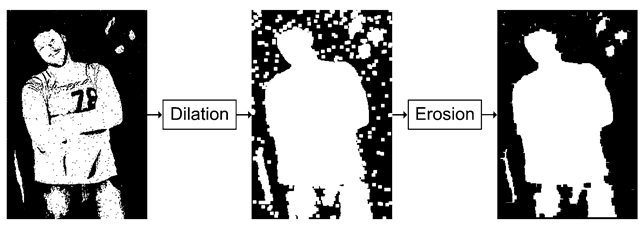
\includegraphics[width=0.7\linewidth]{images/closing}
 	\caption[Morphological closing]{Morphological closing is a combination of \textit{dilation} and \textit{erosion}. Dilation applies a custom-sized binary kernel on a binary input file and turns all \textbf{0} to \textbf{1} as long as at least one \textbf{1} is found in the kernel. Erosion on the other hand turns all \textbf{1} to \textbf{0} in the kernel.\setcitestyle{numbers}Image from \cite{what-when-how.com}\setcitestyle{authoryear}}
 	\label{fig:closing}
 \end{figure}
 Having a look at the different scenarios in the given EPI that can happen when segmenting, the necessity for morphological closing becomes clear, see figure \ref{fig:derivativesfull}. The EPI has two visible disparity transitions, one at pixel [133] and one at pixel [185]. At [133] (a) it is seen that the transition affects multiple neighbouring pixels even though the EPI isn't smoothed yet. Our aim is to mask those transitions. However at Pixel [63] and[174] the threshold is also crossed, since big gradients do not necessarily have to lie on a transition. Still, the false-positive masked transitions are less uncomfortable to handle than a false negative result. It is clearly visible at [63], that zero crossings in the gradient lead to holes in the mask which need to be closed by morphological closing. Since the local environment of each pixel is only given by near pixels in the same segment (masked/unmasked), small holes lead to erroneous results at those pixels. After morphological closing, a last post-processing step has to be made to handle the smearing due to the $3\times 3$-Gaussian pre-smoothing In figure \ref{fig:closing} (d) one sees that the transition peak is Gaussian-formed. If one simply cuts out the segment at the threshold transition, the background segment gradient is still dominated by the gradients directly next to the segment transitions. This becomes visible in figure \ref{fig:segmgaussian}, where the inverted mask of the EPI gradient is shown. Thus, morphological dilation with a $3\times3$ kernel is applied on the inverted filter, resulting in a complete separation of any peak crossing the threshold.
\begin{figure}[h!]
	\centering
	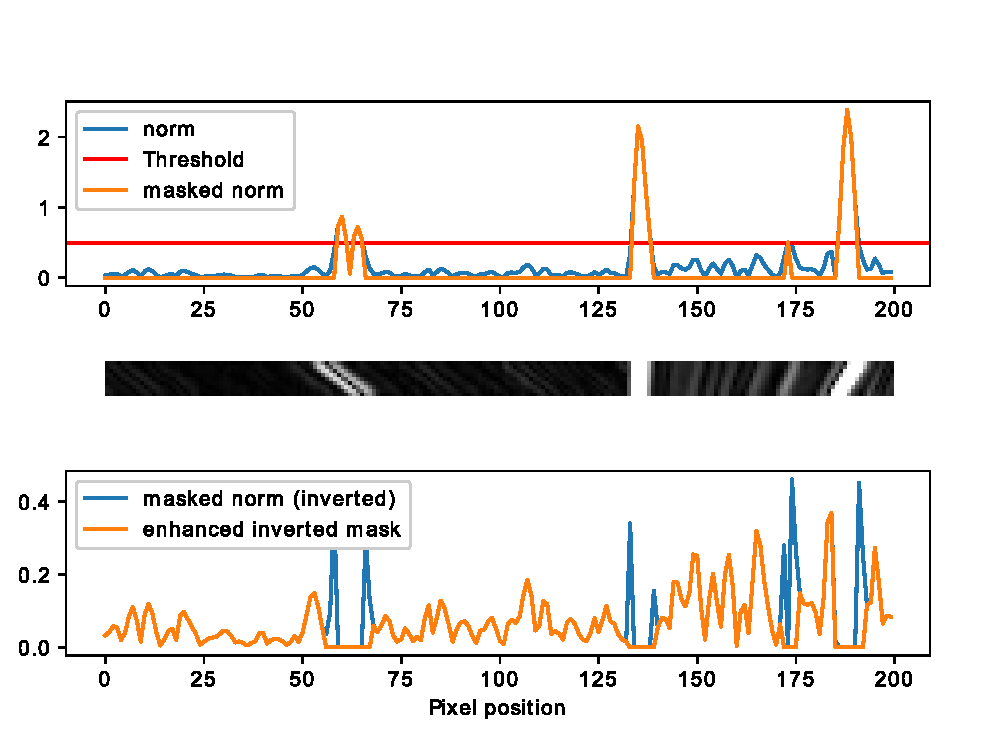
\includegraphics[width=1\linewidth]{images/segm_gaussian}
	\caption[Enhanced segmentation mask]{In the upper diagram the thresholded gradient norm of the EPI (middle) is seen. The norm (masked with the inverted mask) is depicted in the lower figure (blue), while the inverted mask with a dilation filter is depicted in orange.}
	\label{fig:segmgaussian}
\end{figure}
 \subsection{An alternative to the coherence as the confidence measure}
 \label{sec:alternative}
 The coherence (\ref{eq:coherence}) describes how strong the anisotropy of a structure in an image is. In the structure tensor pipeline (section \ref{sec:theo depth}) this value is used as a confidence measure for the corresponding depth value. In this section, we try to define a more profound definition for the confidence based on the distribution of the gradients in a small environment.
 From the structure tensor components we obtain the disparity 
 \begin{equation}\label{eq:disparity2}
 d = \tan\left(\frac{1}{2} \arctan\left( \frac{J_{22}-J_{11}}{2J_{12}}\right)\right),
 \end{equation}
 whose error $\Delta d$ is then given by first order error propagation:
 \begin{equation}\label{eq:err_d}
 \Delta d = \sqrt{\left(\frac{\partial d}{J_{11}}  \Delta J_{11}\right)^2 + \left(\frac{\partial d}{J_{22}}  \Delta J_{22}\right)^2 + \left(\frac{\partial d}{J_{12}} \Delta J_{12}\right)^2 }
 \end{equation}
 When substituting
 \begin{equation}\label{eq:disparity2}
 d = \tan\left(\frac{1}{2} \arctan\left( x\right)\right),\quad \text{with}\quad  x = \frac{J_{22}-J_{11}}{2J_{12}}
 \end{equation}
 we obtain
 \begin{equation}\label{key}
 \frac{\partial d}{\partial x} = 0.5\cdot \frac{d^2+1}{x^2+1}.
 \end{equation}
 With
 \begin{equation}\label{key}
 \frac{\partial x}{\partial J_{11}} = \frac{x}{J_{11} - J_{22}},\quad \frac{\partial x}{\partial J_{22}} = \frac{-x}{J_{11} - J_{22}},\quad  \frac{\partial x}{\partial J_{12}} = \frac{x}{J_{12}}
 \end{equation}
 inserting in \ref{eq:err_d}:
 \begin{equation}\label{eq:deviation_d}
 \Delta d =\sqrt{\left(\frac{0.5\cdot(d^2+1)}{x^2+1}\cdot x\right)^2 \cdot \left(\left|\frac{\Delta J_{12}}{J_{12}}\right|^2 + \left|\frac{\Delta J_{11}}{J_{11}-J_{22}}\right|^2 + \left|\frac{\Delta J_{22}}{J_{11}-J_{22}}\right|^2\right)}
 \end{equation}
 The errors $\Delta J_{11}$, $\Delta J_{12}$ and $\Delta J_{22}$ can be obtained from the statistical deviations of the gradient:
 \begin{align}\label{eq:std_struct}
 \Delta J_{11} &= G *|2\nabla_x|\Delta\nabla_x\\
 \Delta J_{22} &= G *|2\nabla_y|\Delta\nabla_y\\
 \Delta J_{12} &= G *\sqrt{\nabla_x^2\Delta\nabla_y^2 + \nabla_y^2\Delta\nabla_x^2}
 \end{align}
 Those equations are obtained from equation \ref{eq:structuretensor} using first order error propagation. We define $\Delta\nabla_x , \Delta\nabla_y$ as the statistical standard deviation of $\nabla_x, \nabla_y$ in the neighbourhood and calculate it via
 \begin{align}\label{eq:unnormed_std}
 \Delta\nabla_x &= \sqrt{E[\nabla_x^2] - E[\nabla_x]^2}\\
 \Delta\nabla_y &= \sqrt{E[\nabla_y^2] - E[\nabla_y]^2}
 \end{align}
 with the expectation value defined as the Gaussian weighted mean:
 \begin{equation}\label{key}
 E[I] = G* I
 \end{equation}
 However, equation \ref{eq:unnormed_std} only makes sense under the assumption that the underlying distribution of the magnitude whose standard deviation will be computed is close to a normal distribution. This is in general not  the case for the gradient components since deviations in the magnitude of the gradient should not affect on the disparity error estimation. Given that the gradients are normalized, a Gaussian distribution of the gradient around the mean normalized gradient is expected: 
 \begin{align}\label{eq:normed_std}
 \Delta\nabla_{x, \text{normalized}} &= \sqrt{E[\nabla_{x, \text{normalized}}^2] - E[\nabla_{x, \text{normalized}}]^2}\\
 \Delta\nabla_{y, \text{normalized}} &= \sqrt{E[\nabla_{y, \text{normalized}}^2] - E[\nabla_{y, \text{normalized}}]^2}
 \end{align}
 The interrelation between $\Delta\nabla_{y, \text{normalized}}$ and  $\Delta\nabla_x$ is given by
 \begin{align}\label{eq:norm_error}
 \nabla_{x, \text{normalized}} &= \frac{1}{\sqrt{\nabla_x^2 + \nabla_y^2}}\nabla_x \\
 \Delta \nabla_{x, \text{normalized}} &\approx  \frac{1}{\sqrt{\nabla_x^2 + \nabla_y^2}}\Delta\nabla_x,
 \end{align}
 where we neglect the fact that the normalization itself is also erroneous. This simplifies and speeds up the calculation. Equation \ref{eq:norm_error} leads to the expression
 \begin{align}\label{eq:normed_std_final}
 \Delta\nabla_{x} &=  \sqrt{\nabla_x^2 + \nabla_y^2} \cdot \sqrt{E[\nabla_{x, \text{normalized}}^2] - E[\nabla_{x, \text{normalized}}]^2}\\
 \Delta\nabla_{y} &= \sqrt{\nabla_x^2 + \nabla_y^2} \cdot \sqrt{E[\nabla_{y, \text{normalized}}^2] - E[\nabla_{y, \text{normalized}}]^2},
 \end{align}
 which can be calculated from the EPI.
 If we insert the above equation \ref{eq:normed_std_final} into \ref{eq:std_struct} into \ref{eq:deviation_d}, we obtain a deviation measure $\Delta d$ for the disparity based on the gradient deviation in the EPI. At occlusion edges,we expect a bimodal distribution of the gradient, such that the deviation $\Delta \nabla_{x/y, \text{normalized}}$ should be large. Thus the new error measure should handle occlusion edges as well.
 
 \subsection{Alternative merging of x- and y- orientation}
 In the old ST pipeline, the coherence value as defined in equation \ref{eq:coherence} not only determines which depth value should be chosen from refocussing the EPI, it is also used to decide whether the local depth estimation is taken from the x-directed EPI or the y-direction. In the article of \cite{sheng2018occlusion} a full light field is evaluated such that multiple EPIs are available for each point. To handle occlusions, the EPI with less intensity variance is chosen to calculate the depth. As we are working with a crosshair light field only providing two EPIs for each scene point, this is not a possible approach in our case. Choosing the one with higher coherence seems logical, however at occlusions we are mostly provided with a clear structure in the EPI leading to a high coherence value. As a result, the EPI including edges is chosen in the close neighbourhood of a discontinuity edge, leading to 'edge fattening'.\\
 In his work, \cite{wanner2014orientation} also proposes a TV-L minimization scheme to merge the disparity values resulting from x-directional and y-directional EPIs. Despite achieving good results, the improvement did not justify the calculation time of this optimization scheme. He thus sticks to choose the value with higher coherence.\\
 Instead, we propose to choose the disparity value which relates to a larger depth and only chooses the closer disparity value, if the coherence difference is big enough. Therefore we introduce a threshold:
 \begin{equation}\label{eq:altmerging}
 d(x,y) = \begin{cases}
 \min(d_x(x,y),d_y(x,y))&\text{ if } |c_x(x,y)-c_y(x,y)|<\text{threshold} \\
  d_x(x,y)&\text{ else, if } c_x(x,y)> c_y(x,y)\\
  d_y(x,y)&\text{ else}\\
  \end{cases}
   \end{equation}

\begin{figure}[h!]
	\centering
	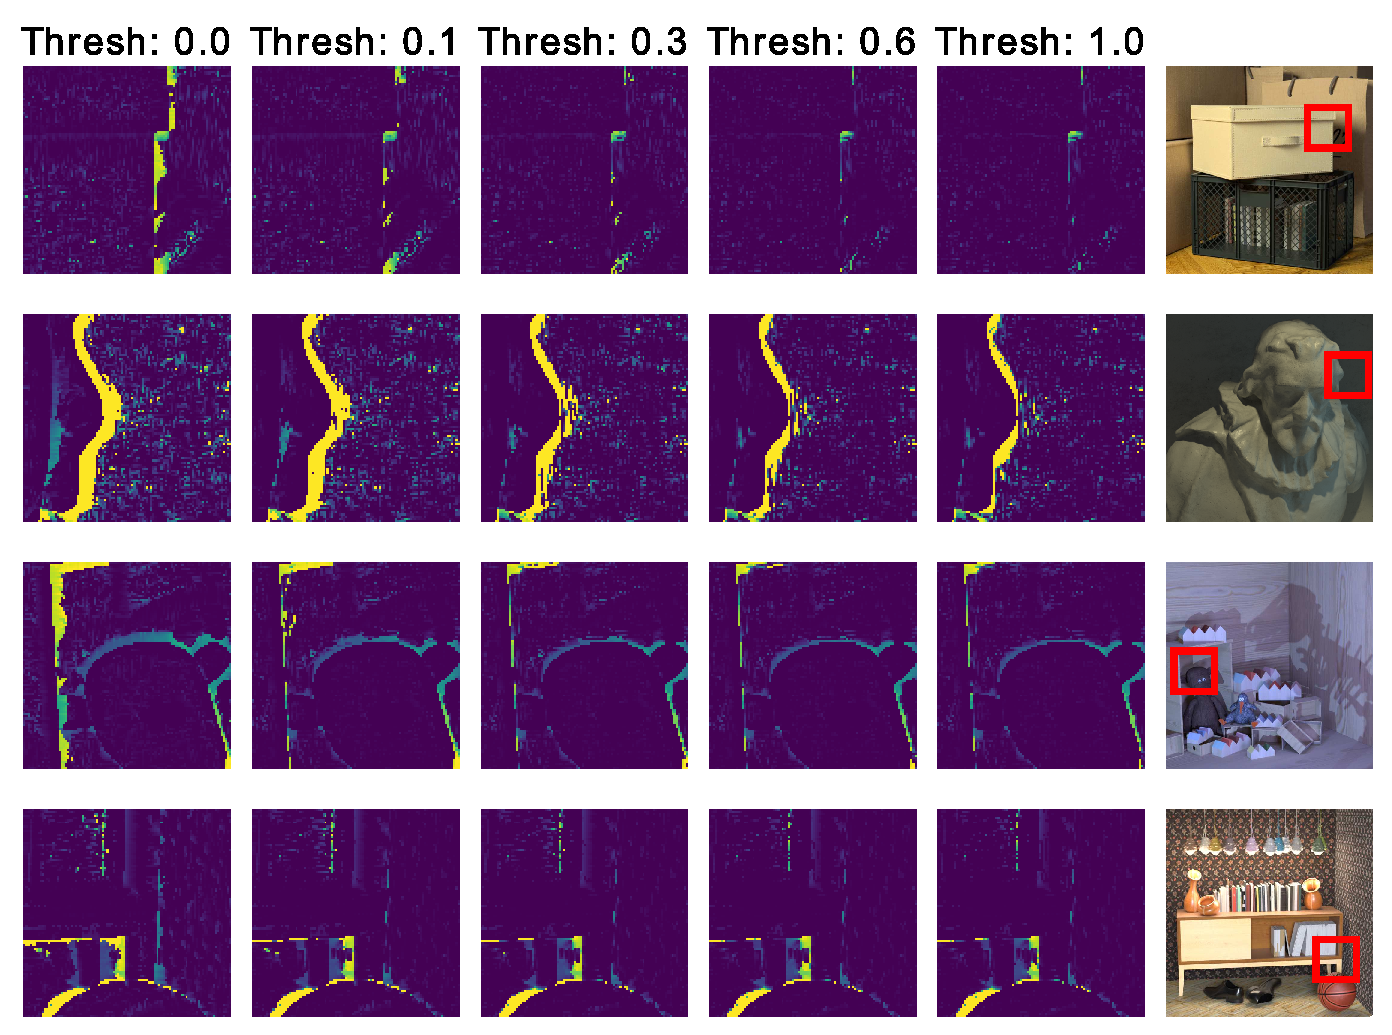
\includegraphics[width=1\linewidth]{images/choose_lower_difference}
	\caption[Alternative Merging: Parameter dependence]{From left to right: Parameter dependent alternative merging. Up to down: scenes \textit{boxes, cotton, dino, sideboard}. The deviation from ground truth is marked yellow, zero deviation is dark-purple.}
	\label{fig:chooselowerdifference-eps-converted-to}
\end{figure}

 Figure \ref{fig:chooselowerdifference-eps-converted-to} shows the effect of varying the threshold introduced in equation \ref{eq:altmerging} on the depth map by showing the deviation to the ground truth at occlusion discontinuities for different parameter values. The occlusion edges shrink significantly with a higher threshold. However, the effect is scene-dependent.
\section{Depth from focus}
\label{sec:theo depth}
One advantage of using light fields for depth measure is its ability to get a two-dimensional mapping of the scene with focus at any depth. Integrating the views of the light field camera array has the same effect as the integration of a focussed lens camera, as the lens is simply integrating slightly different viewpoints of the same scene point when focussed on the correct depth. \\
 Obtaining the refocussed integrated image is a synthetic process that only requires shifting the view coordinates artificially. Given a full four-dimensional light field $L(u, v, x, y)$ we can refocus the light field as described in\setcitestyle{numbers}\cite{ng2005light}\setcitestyle{authoryear}:
 \begin{equation}\label{eq:refocus}
L'(u, v, x, y) = L(u(1-d'), v(1-d'), x, y),
\end{equation}
where $d'$ describes the relative pixel shift. The disparity is directly related to the absolute depth of the focus if the relevant camera parameters are known. Given the baseline $b$ in meters and the focal length $f$ in pixels, the depth $Z$ is given as \begin{equation}\label{key}
Z = \frac{f\cdot b}{d}.
\end{equation} 
We obtain
\begin{equation}\label{key}
\bar{L}(x,y) = \frac{1}{N_{u,v}}\int\int L'(u, v, x, y) du  dv =\frac{1}{N_{u,v}}\sum_{u}\sum_{v}  L'(u, v, x, y)
\end{equation}
Once we can focus at any range, one can adopt \textit{depth-from-focus}-techniques as described in \cite{watanabe1998rational} for depth measure. If the scene point at a given image coordinate $(x, y)$ in the centre view is in focus, the contrast in the integrated image $\bar{L}(x,y)$ is high, thus a contrast measure at each pixel combined with stepwise refocussing yields a depth map. \\
For measuring the contrast, one has different options: The most straightforward approach is calculating the first derivative of the grey-value image. At high contrast structure, the local intensity changes are expected to be high. Alternatively one could measure the second derivative Laplacian that eventually results in higher robustness. The implementation and tests of those techniques for the benchmark dataset can be found in section \ref{sec: depth from focus}.\\
Using a pinhole camera array allows us to go further and find a response value that shows higher consistency. Taking the absolute difference between the centre view of the camera array and the refocussed image yields promising results as shown in \cite{tao2017shape}. Under the assumption of Lambertian surfaces, the RGB value of any scene point should be the same under all angles. Thus when refocussed on the correct depth, summing over all angles should result in a value that ideally is the same as in the centre view alone. This is referred to as \textit{photo consistency}; for more information read \cite{tao2017shape}.
The response value at a given depth is obtained from
\begin{equation}\label{key}
D'(x,y) = \frac{1}{|W_D|}\sum_{x',y' \in W_D} \left|\bar{L}(x',y')- P(x', y')\right|,
\end{equation}
where $P(x,  y)$ is the centre view. For more robustness, it is averaged over a small window. Note that calculating the norm results in a 1-channel-image while the input images are RGB-images. \\ Tao et al. propose another measure that they refer to as \textit{angular correspondence}. It follows the same principle, but instead of integrating the refocussed light field followed by comparing it to the centre view, they directly take the difference of each viewpoint to the centre view and sum up those differences:
\begin{equation}\label{eq:responsecorr}
D'(x,y) = \frac{1}{N_{u,v}}\sum_{u}\sum_{v}  \left|L'(u, v, x, y) - P(x,y)\right|.
\end{equation}
We tested those methods against the common contrast measures mentioned above, the results are found in section \ref{sec: depth from focus}.

\section{Semi-global matching}
\subsection{Semi-global matching for stereo vision}
In contrast to light field depth estimation techniques stereo systems more often suffer from mismatching pixels between the left and right images. Many attempts have been made to smoothen bad pixels, resulting in blurred edges or long calculation times. One promising attempt to improve matching results was published by \cite{hirschmuller2005accurate}: we speak of semi-global matching (SGM).
\begin{figure}[h!]
	\centering
	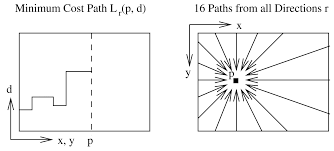
\includegraphics[width=0.7\linewidth]{images/sgm_paths}
	\caption[SGM Path explanation]{Left: Minimum cost path along an exemplary scanline. Right: each point gets passed by multiple paths from different directions. Image from\setcitestyle{numbers}\cite{hirschmuller2008stereo}\setcitestyle{authoryear}}
	\label{fig:sgmpaths}
\end{figure}
In general,  matching of two stereo images means shifting the disparity over the predefined disparity range and comparing both images (pixel- or block-wise) until we have a cost value at each image point for each discrete disparity. We assign to each pixel $\vec{p}$ the disparity value $D_{\vec p}$ which is related to the lowest cost $C(\vec{p}, D_{\vec p})$. This matching does not have to be unique, resulting in erroneous pixel disparities. 
To overcome this one wants to minimize a global cost function of the form 
\begin{equation}\label{eq:global_sgm}
E(D) = \sum_{\vec p} \left(C(\vec{p}, D_{\vec p}) + \sum_{q\in N_p} 
\begin{cases}
	P1 & \text{ if }|D_{\vec p} - D_{\vec q}| = 1\\
	P2 & \text{ if }|D_{\vec p} - D_{\vec q}| \geq 1\\
	0 & \text{ else }
	\end{cases}  
\right).
\end{equation}
The fist term sums all matching costs over the whole image, while the second term forces continuity by comparing the disparity of all neighbour pixels $N_q$ to the disparity $D_p$; if a  small discontinuity is detected ($D_{\vec p} - D_{\vec q} = 1$), a small penalty is added to the global cost function. Since a small discontinuity can be found essentially at any tilted plane, only a small error is added. A bigger disparity difference indices a clear discontinuity in the disparity map. Note that the penalty $P2$ can be divided by the gradient $|\nabla|$ of the original image to allow a disparity discontinuity when we find edges in the image; at these points we expect the disparity to be discontinuous. We obtain
\begin{equation}\label{eq:stereosgm_p2}
P2'(x,y) = \frac{P2}{|\nabla|(x,y)}.
\end{equation}\\ However, minimizing the global cost function involves computational cumbersome algorithms as it is an NP-complete Problem (\cite{hirschmuller2011semi}). Semi-global matching however chooses another approach by minimizing the global cost function along one-dimensional lines -- this can indeed be calculated in polynomial time.
The new smoothed cost function $S(\vec p , D_{\vec p})$ at pixel $\vec{p}$ is then given as the sum of all 1D minimum cost paths that are ending in $\vec{p}$.  The minimal cost $L'_r$ along the path $r$ is defined recursively as
\begin{equation}\label{eq:local_sgm}
L'_r(\vec{p}, D) = C(\vec{p}, D) + \text {min}
\begin{cases}
	L'_r(\vec{p}_\text{before}, D) \\
	L'_r(\vec{p}_\text{before}, D+1)+P1 \\
	L'_r(\vec{p}_\text{before}, D-1)+P1 \\
	\text{min}_i L'_r(\vec{p}_\text{before}, i)+P2 
\end{cases}
\end{equation} 
By always adding the minimum path cost of the previous pixel on the scanline we are looking at, we solve equation \ref{eq:global_sgm} in one dimension. Note that the rolling sum can reach quite high numbers that are unpleasant to handle on the computer; a normalization is implemented by subtracting min$_D L'_r(\vec{p_\text{before}}, D)$ from all pixel cost values $L'_r(\vec{p}, D)$. The position of the minimum cost function at pixel $\vec p$ is unaffected by that normalization. In figure \ref{fig:sgmpaths} an exemplary scanline is shown on the left.  The point $p$ is reached by 16 paths, whose cost functions $L'_r(\vec{p}, D)$ are cumulated (figure \ref{fig:sgmpaths} right).
\subsection{Semi-global matching for light fields}
Even though Hirschmüller describes SGM as a complete algorithm to obtain a disparity map from a stereo image input, we further refer to SGM as the true novelty of his work: The implementation of an approximation to the global solution of the cost function (equation \ref{eq:global_sgm}). Independent from the method one uses to calculate a disparity map,  one needs a cost function defined in disparity space for each pixel to make use of SGM. 
Similar to the Stereo matching depth estimation, the structure tensor depth estimation pipeline for light field data sets produces a disparity map and a coherence value at each disparity shift. This implies that the SGM algorithm can be adapted to improve the results of the structure tensor pipeline. However, there are some significant differences between these two methods:
\begin{enumerate}
	\item The structure tensor algorithm is tuned to a much smaller disparity range. While \cite{hirschmuller2005accurate} scans a disparity range of 32 pixels, the benchmark data sets for light fields mostly include close-up views of objects, with a disparity range between 2 and 10 pixels. In figure \ref{fig:table-skizze} one can see the different values that are allocated in memory for each pixel of the image.
	\item The sub-pixel accuracy using the structure tensor is a lot higher than the stereo matching sub-pixel accuracy. A simple adaptation of the algorithm to the structure tensor pipeline would require to give up the best feature that is provided by the ST, its sub-pixel accuracy.
\end{enumerate}
\begin{figure}[h!]
	\centering
	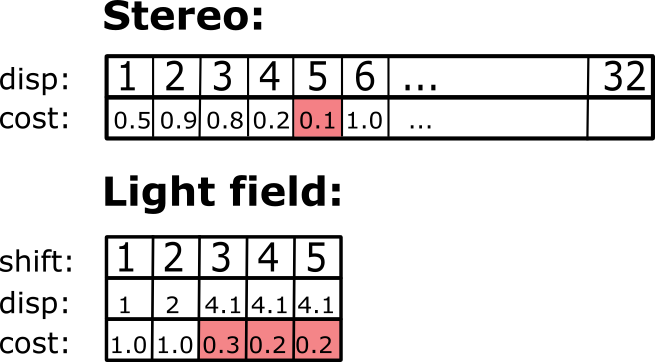
\includegraphics[width=0.5\linewidth]{images/sgm_table}
	\caption[SGM data to be storaged]{SGM data that needs to be scored at each pixel in case of stereo (upper) and light field (lower). The cost values related to the 'correct' disparity are marked red.}
	\label{fig:table-skizze}
\end{figure}

To handle those problems, we do not throw away the sub-pixel accuracy. Instead, we use the float-value disparities to decide whether we penalize a disparity discontinuity or not. As one can see in figure \ref{fig:table-skizze}, we have to process additional information, since the exact disparity value is not implicitly given by the index of the allocated cost value (in contrast to the original algorithm). Switching to a continuous space requires a new definition of the global cost function we defined in equation \ref{eq:global_sgm}.
%\begin{figure}[h!]
%	\centering
%	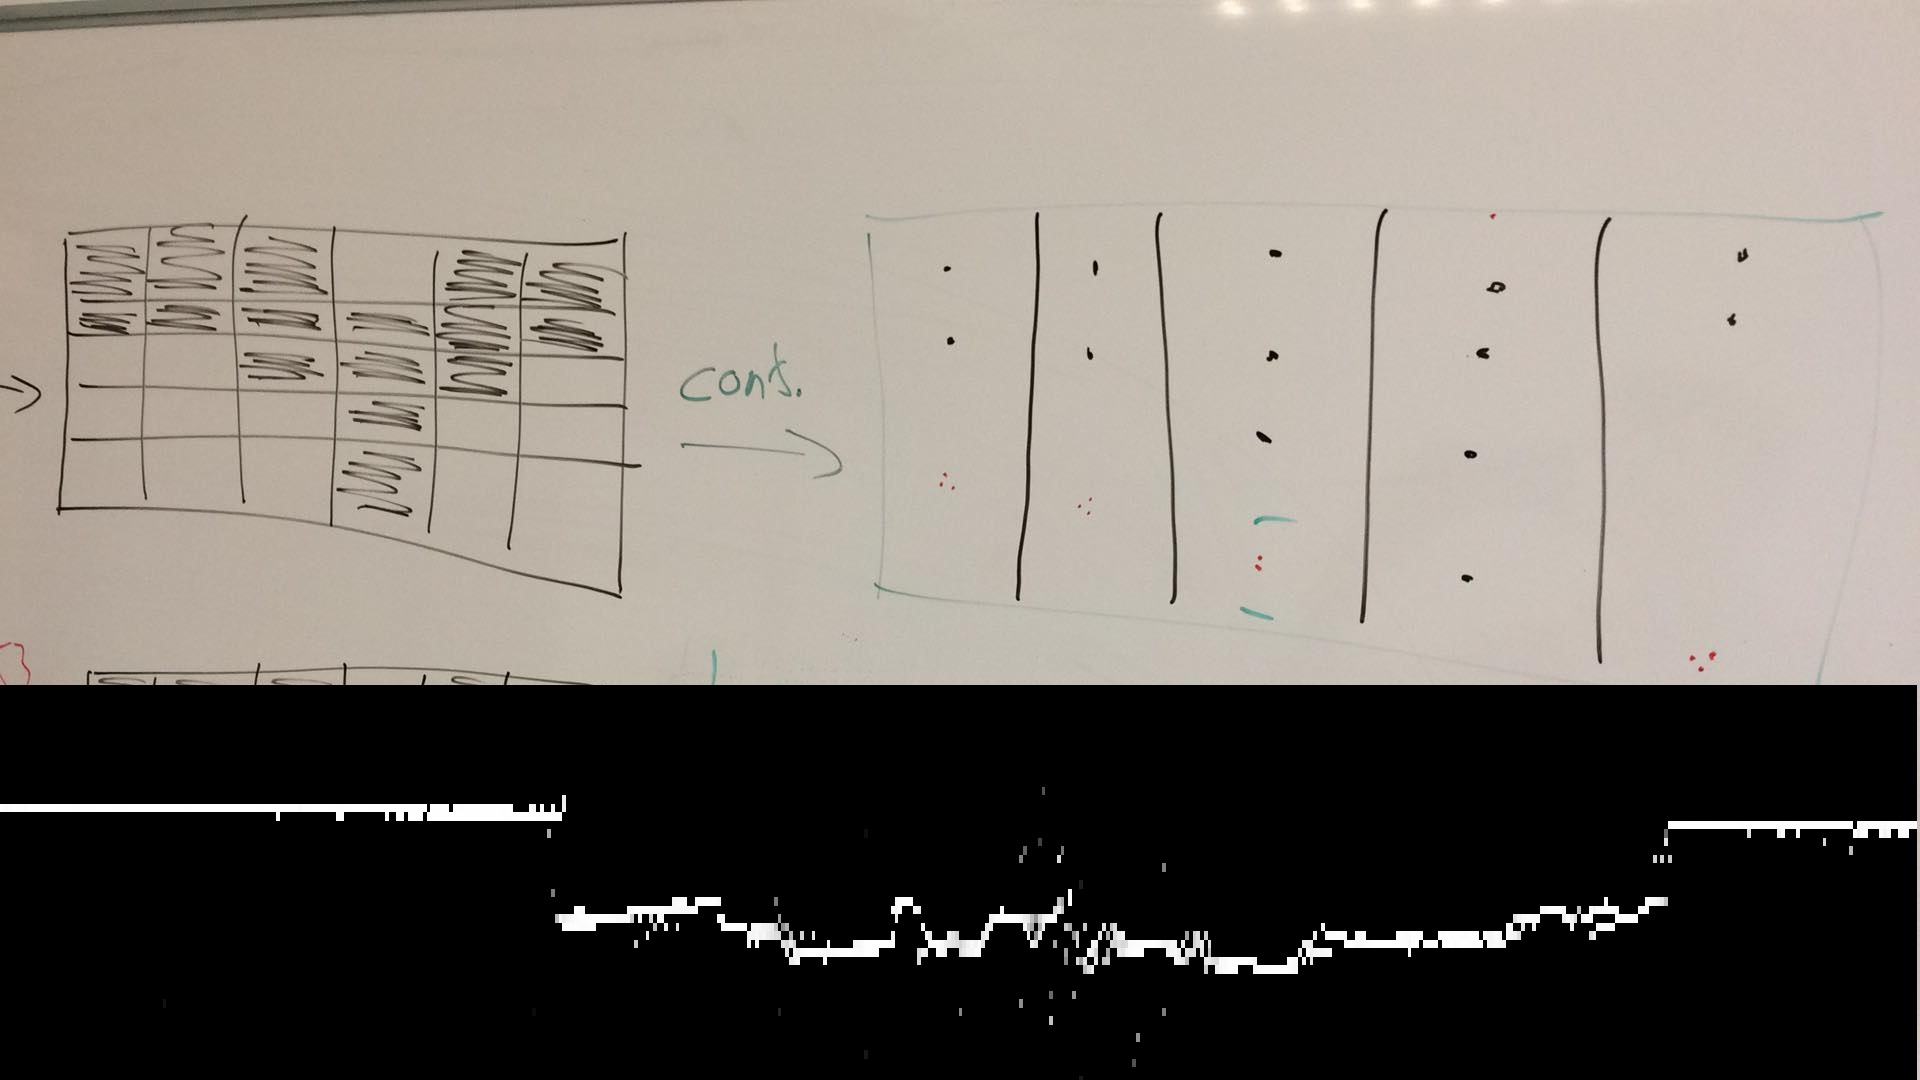
\includegraphics[width=0.7\linewidth]{images/discrete_cont}
%	\caption[Discrete scanline to continuous scanline]{In this figure one can see the sketch of one arbitrary scanline of the structure tensor method. Under the Assumption that the ST algorithm recognizes the structure of the EPI perfectly, we either have two or three disparity shifts that have a high coherence (coloured white) (a) and result in approximately the same final disparity. This can be seen if we plot the exact disparity values in a continuous space(b). In (c) real data scanline cost is plotted with a resolution of ca. 100 pixels.}
%	\label{fig:discretecont}
%\end{figure}

\begin{figure}[h!]
	\centering
	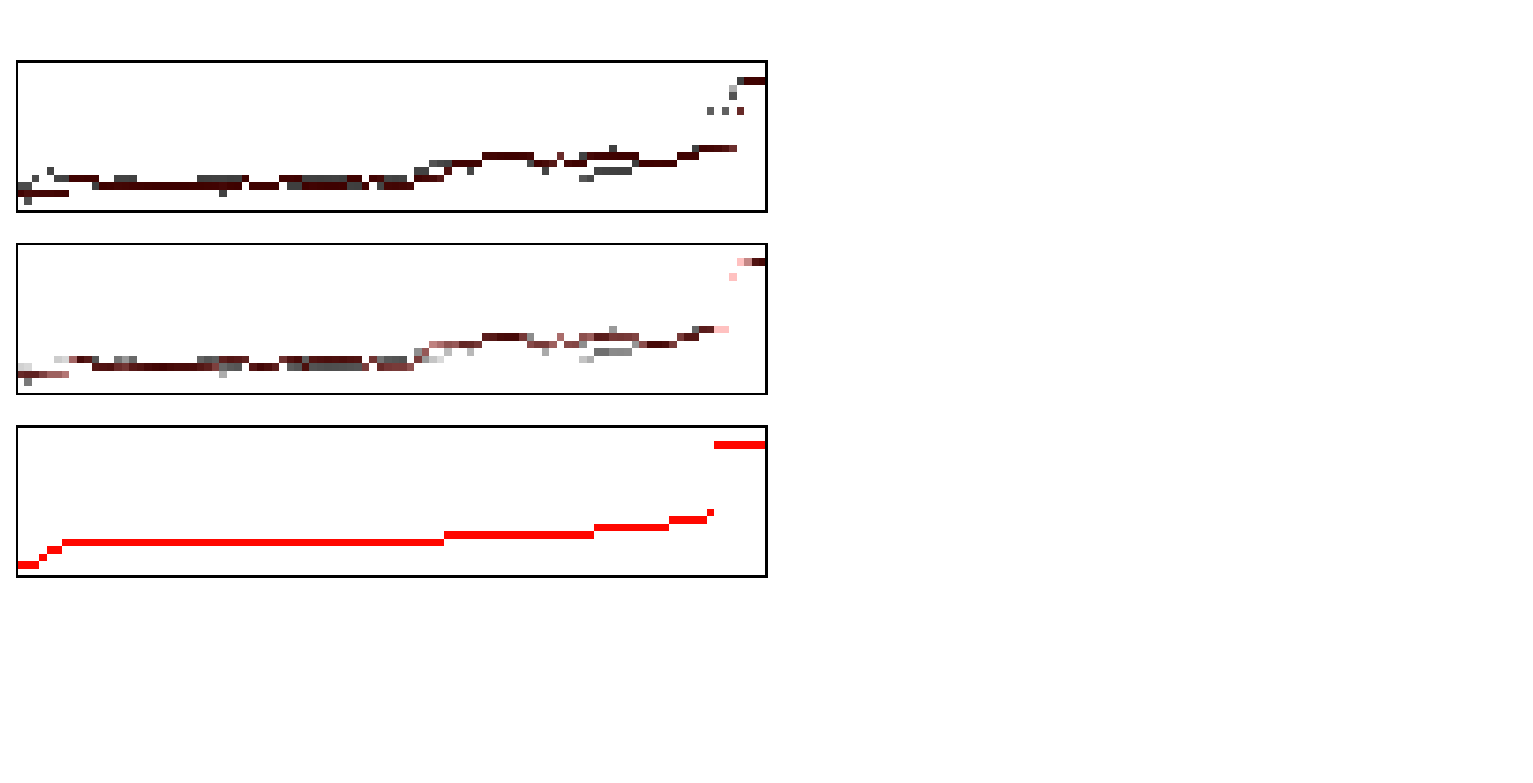
\includegraphics[width=0.6\linewidth]{images/pens_paths}
	\caption[Exemplary SGM path]{Upper: Measured disparity path (red) with underlying candidate values (grey). The intensity of the grey value reflects the cost value. Middle: disparity Paht after running SGM. Lower: Ground truth path}
	\label{fig:penspaths}
\end{figure}



 In the following, we refer to $s$ as the disparity shift in the ST algorithm. Note that we replaced $D$ by $d$ to clarify that the disparity is no longer discrete:

\begin{equation}\label{eq:global_sgm_cont}
E(d) = \sum_{\vec p} \left(C(\vec{p}, d_{\vec p}) + \sum_{q\in N_p} 
\begin{cases}
P1\cdot |d_{\vec p} - d_{\vec q}|  & \text{ if }|d_{\vec p} - d_{\vec q}| \leq 1\\
P2 & \text{ if }|d_{\vec p} - d_{\vec q}| > 1\\
\end{cases}  
\right).
\end{equation}
The recursive 1-d form to solve the global constraint on a scanline then changes to:

\begin{equation}\label{eq:recursive1d}
L'_r(\vec{p}, s) = C(\vec{p}, s) + \text{min}_i
\begin{cases}
L'_r(\vec{p}_\text{before}, s_i)+P1 \cdot |d_{\vec p, s} - d_{\vec{p}_\text{before}, s_i}|  & \text{ if }|d_{\vec p, s} - d_{\vec{p}_\text{before}, s_i}| \leq 1 \\
L'_r(\vec{p}_\text{before}, s_i)+P2 & \text{ if }|d_{\vec p, s} - d_{\vec{p}_\text{before}, s_i}| > 1
\end{cases}
\end{equation} 
The biggest difference lies in the fact that the small factor that is smoothing the image linearly increases with the distance. This change is necessary under the assumption that the disparity space is continuous. In other words we cluster disparity differences between two neighbouring points as either part of one surface ($|d_{\vec p, s} - d_{\vec{p}_\text{before}, s_i}| \leq 1$) that gets smoothed by the linearly increasing penalty, or assume a real disparity discontinuity that is penalized regardless of the size of the jump - the second error remains constant as it is in stereo matching. Note that $P2$ is modified as before (equation \ref{eq:stereosgm_p2}) by 
\begin{equation}\label{eq:gradientp2}
P2'(x,y) = \frac{P2}{|\nabla|(x,y)}.
\end{equation}
with $|\nabla|(x,y)$ being the centre view colour difference
 \begin{equation}\label{key}
 |\nabla|(x,y) = \sqrt{\left(C_b(\vec p) - C_b(\vec p_\text{before})\right)^2 + \left(C_g(\vec p) - C_g(\vec p_\text{before})\right)^2+ \left(C_r(\vec p) - C_r(\vec p_\text{before})\right)^2}
 \end{equation}
  $C_\text{\{b,g,r\}}$ are the blue, red and green colour channels of the centre view, respectively. The penalty for a disparity discontinuity is lowered if the colour intensity difference at this discontinuity is high. In figure \ref{fig:penspaths} an exemplary scanline path through the scene \textit{pens} is shown before and after using SGM. The position of the disparity candidates along the scanline are shown. While in the upper row we see a lot of ambiguities, in the lower row (after using SGM) a clear continuous path comes to light. Figure \ref{fig:subplotsgm} shows that each path for itself leads to tearing effects in the given path direction. Only after merging all cost values from the different paths we obtain a smooth depth map while maintaining sharp edges.
\begin{figure}[h!]
	\centering
	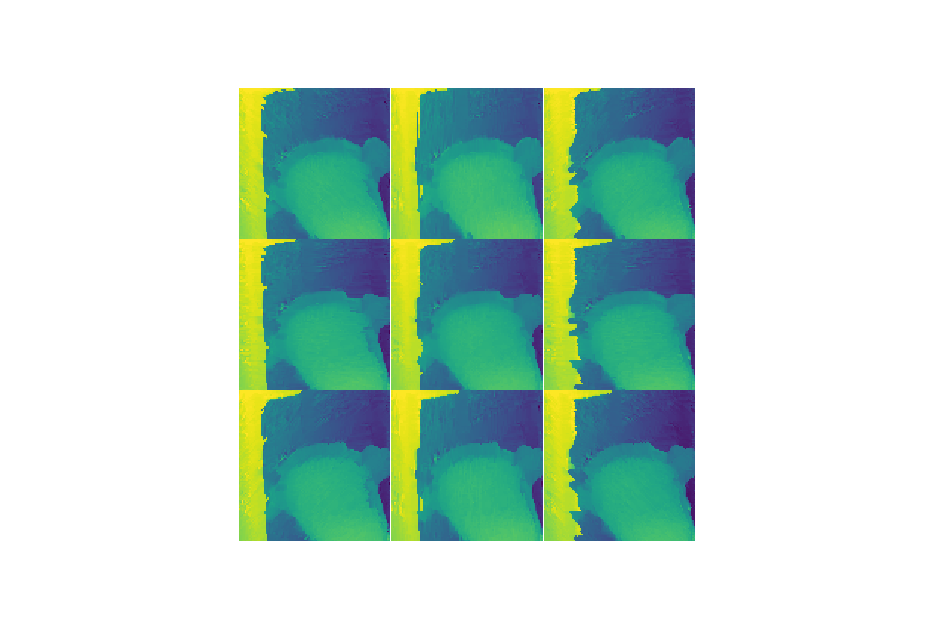
\includegraphics[width=1\linewidth]{images/subplot_sgm}
	\caption[SGM depth map from different directions]{a) Depth map of scene \textit{dino} using the old ST pipeline. b) Depth maps after using SGM only in one direction, respectively. c) Depth map after running SGM, using 8 paths.}
	\label{fig:subplotsgm}
\end{figure}

\subsection{Occlusion awareness in SGM for light fields}
\label{sec:semiglobal3}
As discussed in section \ref{sec:occlusionawareness} the foreground structure is often dominating near disparity discontinuities. However, the structure tensor still finds the background structure near the boundary within a different SGM shift. With both disparity values stored at pixel $p$ with different costs, the foreground is chosen more often.\\
The simple heuristic approach is to change the global minimization function \ref{eq:global_sgm_cont} such that a positive disparity jump is less punished than a negative one. In fact, the function changes to
\begin{equation}\label{eq:global_sgm_cont_occlusion}
E(d) = \sum_{\vec p} \left(C(\vec{p}, d_{\vec p}) + \sum_{q\in N_p} 
\begin{cases}
P1\cdot |d_{\vec p} - d_{\vec q}|  & \text{ if }|d_{\vec p} - d_{\vec q}| \leq 1\\
P2 & \text{ if }d_{\vec p} - d_{\vec q} > 1\\
P3 & \text{ if }d_{\vec p} - d_{\vec q} < -1\\
\end{cases}  
\right).
\end{equation}
\subsection{SGM as post-processing smoothing}
\label{sec:postprocessing_smoothing}
\begin{figure}[h!]
	\centering
	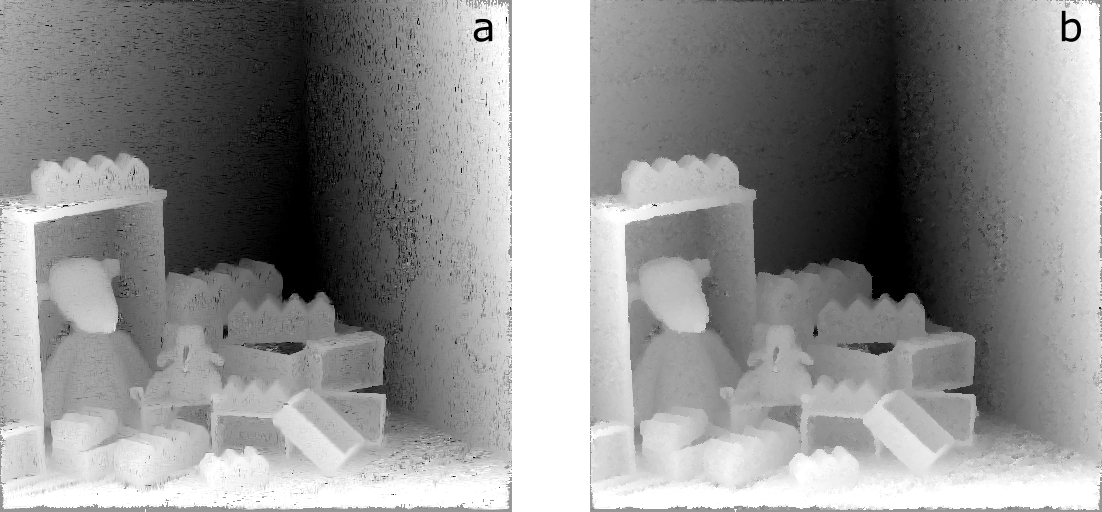
\includegraphics[width=1\linewidth]{images/sgm_ppr_example}
	\caption[Example for post-processing smoothing]{a) Erroneous disparity map before smoothing. b) Same disparity map after smoothing.}
	\label{fig:sgmpprexample}
\end{figure}
Minimizing the global energy function by solving it along different paths is possible as long as for each point a disparity candidate list with cost values is given. In general, it is possible to extract those candidate values in a post-processing step by evaluating the close neighbourhood of a point in the disparity map. In the scope of this work, we propose to choose for each pixel 5 neighbouring pixels that are randomly chosen from the close neighbourhood after constructing the disparity map. In this sense, the SGM is used as a pure post-processing step that can be used to improve any depth map, regardless of the underlying algorithm for depth reconstruction. The effect of smoothing the disparity map while maintaining edges is depicted in figure \ref{fig:sgmpprexample} as an example.
\subsection{Iterative post-processing}
\label{sec:iterative}
To reach the best result possible the SGM post-processing is applied multiple times. This iterative processing is inspired by the work of \cite{freist2018reconst} that uses graph cutting to optimize the depth map. Instead of choosing random pixels from the close neighbourhood, the candidate values are found by adding/subtracting a $\Delta$ from the original pixel depth value $d_{i}$, such that the candidate values are given by the triple $(d_{i};d_{i}-\Delta;d_{i}+\Delta)$. The candidate with the lowest cost is chosen and new candidates are formed for the next iteration. To reach convergence, $\Delta$ shrinks by a factor of two each iteration as long as the chosen candidate was the central one. Otherwise, $\Delta$ stays the same size. In figure \ref{fig:iterationsteps} a) an exemplary disparity value is shown in dependence of the iteration step. The candidate window gets smaller each step, the stopping criterion is given by the overall iteration number. 
\begin{figure}[h!]
	\centering
	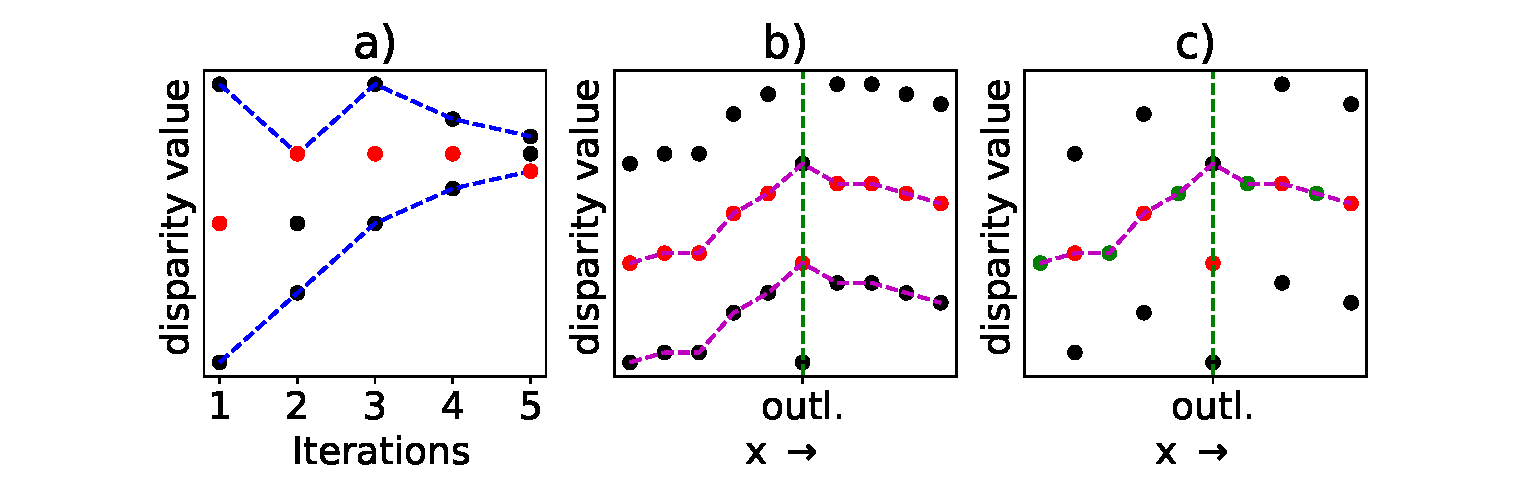
\includegraphics[width=1\linewidth]{images/iteration_steps}
	\caption[Iterative SGM: Convergence]{a) One exemplary pixel value in function of iteration steps. At each iteration, 3 candidate values for each pixel are chosen, the one with the lowest score is marked red. The candidate value window is marked with blue lines. b) One exemplary scanline through the depth map. Red marks the input values, the black points are the added candidate values. The green line marks the position of an outlier. The magenta-coloured lines show the paths with the lowest cost. c) same as the diagram b) with the difference of using a chess pattern initialisation. }
	\label{fig:iterationsteps}
\end{figure}
However, setting the same $\Delta$ at each pixel leads to problems along any SGM scanline, as sketched in figure \ref{fig:iterationsteps} b). Since all candidates are initialized with the same $\Delta$ one finds 3 identical surfaces through the scanline that are shifted by $\Delta$. Since they are almost identical, the cost of the disparity values lying either on one or the other surface is close to being identical. Hence the algorithm produces large errors along the scanline when choosing the wrong 'layer'. To overcome this problem one could apply a chess-pattern-like initialisation of the pixels. When proposing candidates to the SGM algorithm, every second pixel in the 2D-depth map is held constant to one value while the other pixels obtain 3 candidate values. After iterating, the second half of the pixels will be held constant. As depicted in figure \ref{fig:iterationsteps} c) only one surface line will have a low cost value. Doing this iteration, though, doubles the amount of time the code consumes. 
\subsection{A new penalty function} 
The iterative pipeline does not assume that any of its candidates at one pixel position have to be close to the ground truth disparity, e.g. having an outlier $d_i$ at pixel $i(x,y)$ does not necessarily mean that either $d_i-\Delta$ or $d_i+\Delta$ are close to the ground truth. With punishing those candidates as described in equation \ref{eq:global_sgm_cont}, all 3 candidates would obtain the same cost function value. However, one wants the candidate that is closest to its neighbours to be the one with the lowest cost. Thus, the cost function should be monotonically increasing as function of the distance to the previous disparity value $d_{i-1}$. A simple linearly increasing cost function would lead to overly smoothed edges. The proposed global cost function that is to be minimized then looks like

\begin{equation}\label{eq:global_sgm_function}
E(d) = \sum_{\vec p} \left(C(\vec{p}, D_{\vec p}) + \sum_{q\in N_p} 
P2\cdot \left(1- \exp\left(\frac{-|d_{\vec{p}} - d_{\vec{q}}|}{P1}\right)\right)
\right).
\end{equation}
Note that the initial cost can be neglected since we assume the same initial cost for all candidates such that we obtain the form
\begin{equation}\label{eq:global_sgm_function_wo}
E(d) = \sum_{\vec p}\sum_{q\in N_p} 
P2\cdot \left(1- \exp\left(\frac{-|d_{\vec{p}} - d_{\vec{q}}|}{P1}\right)\right)
\end{equation}
with the 1D recursive form
\begin{equation}\label{eq:recursive1dexp}
L'_r(\vec{p}, s) = \text{min}_i\left( L'_r(\vec{p}_\text{before}, s_i) + P2\cdot \left(1- \exp\left(\frac{-|d_{\vec{p,s}} - d_{\vec{p}_\text{before}, s_i}|}{P1}\right)\right)\right).
\end{equation}
The equation \ref{eq:recursive1dexp} is plotted in figure \ref{fig:penaltyfunction} on the right side. 
\begin{figure}[h!]
	\centering
	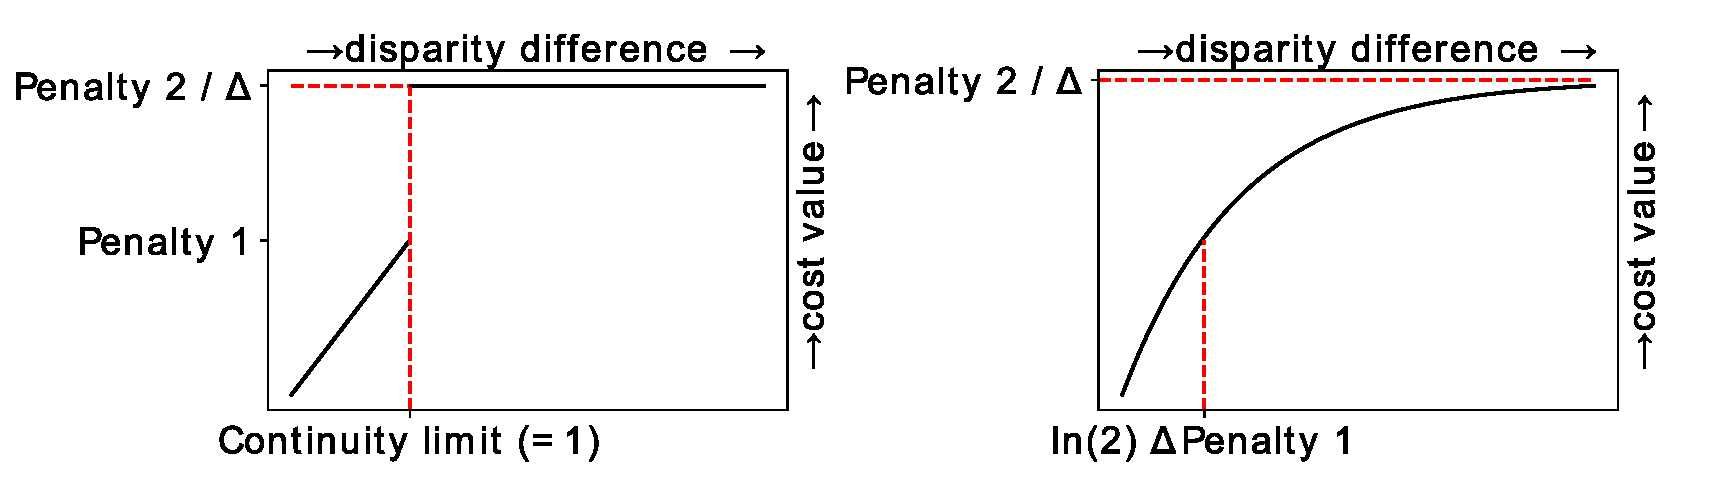
\includegraphics[width=1\linewidth]{images/penalty_function}
	\caption[Iterative SGM: Penalty function]{Sketch of different proposed Penalty functions. Left: Function as described in equation \ref{eq:recursive1d}. Right function as described in \ref{eq:recursive1dexp}.}
	\label{fig:penaltyfunction}
\end{figure}
In comparison to the old penalty function it has one less parameter, it is continuous and it always favours smaller disparity differences in order to get iterative processing to work. The error $P2$ is modified the same way as before, see equation \ref{eq:gradientp2}. Large image gradients are more likely to lie on a disparity discontinuity, therefore the error is reduced.
In figure \ref{fig:lineariteration} the effect of different penalty functions is depicted. Figure \ref{fig:lineariteration} a) shows the result of the scene $dino$ after smoothing with the exponential penalty function \ref{eq:recursive1dexp}, while figure \ref{fig:lineariteration} b) shows the disparity map after iterative SGM processing with a linear penalty function. One sees that the linear function leads to smoother surfaces, however the smoothness constraint also oversmoothens the edges in the image. In a) the edges are maintained sharp. The figure \ref{fig:lineariteration} c) shows the ground truth for comparison. 
\begin{figure}[h!]
	\centering
	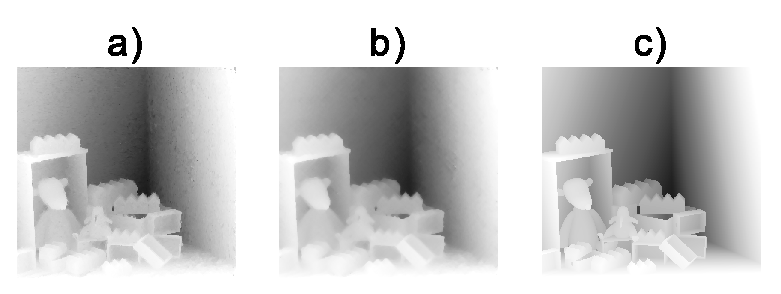
\includegraphics[width=1\linewidth]{images/linear_iteration}
	\caption[Linear cost function vs. exponential cost function results]{a) Depth map after iterative SGM smoothing using an exponential penalty function. b) Instead, a linear penalty function is used. c) Ground truth}
	\label{fig:lineariteration}
\end{figure}
\subsection{Semi-global matching implementation}
\label{sec:SGM_implement}
The implementation for using semi-global matching in our work is in line with the open source implementation published by \cite{sgmimplement}. This code, however, uses only 8 instead of 16 paths along the image. \cite{hirschmuller2005accurate} claims to reach computation times that are around 20 times faster than the implementation of Moratto with comparable hardware set-up\setcitestyle{numbers}(source: \cite{sgmimplement}), neither do we achieve fast computation times.\setcitestyle{authoryear}Further, \cite{ernst2008mutual} implement the SGM algorithm on a GPU leading to an enormous increase of efficiency. Since all paths can be calculated in parallel, a GPU implementation can be implemented in a straightforward manner. The programming of the GPU implementation exceeds the boundaries of this work and will be part of future research and development. Instead, we focus on the feasibility of implementing SGM for light fields.
\section{Metrics for the evaluation of depth maps}
In the following, technical dataset details and general evaluation measures are presented. The datasets are provided by \cite{honauer2016benchmark}.
\subsection{Dense and sparse depth maps}
The synthetic light field datasets are designed with  \cite{blender2014blender} and provide photos from the scene in a crosshair pattern, similar to the camera configuration in figure \ref{fig:lumiplus}. In contrast to stereo camera setups, light field imaging enables a densely sampled reconstruction of the depth at each pixel. However, a full point cloud of a scanned object which is ideal for object detection applications will not be reconstructed due to occlusions. To evaluate the quality of the depth map, one could either try to optimize the overall error on the whole depth map (MSE) or count the number of pixels that are close to the Ground Truth with given tolerance Level (BadPixel score). From thereon one either tries to provide a sparse depth map masking out all the pixel where the confidence is low or the disparity map is provided on the whole pixel space. While sparse disparity maps are the choice for exact measurements in industrial applications, the second method facilitates comparisons of different methods. For this reason, the thesis mainly focusses on the metric score on the dense disparity estimation maps using different algorithms. Only for the application on real data one has to face large regions with low confidence, thus masking becomes relevant again.
\subsection{Mean squared error}
The Mean squared error, typically multiplied by a factor of 100, is defined as 
\begin{equation}\label{key}
\text{MSE} = \frac{\sum_x (d(x) - gt(x))^2}{\text{Nr of Pixels}} \cdot 100
\end{equation}
and describes the overall deviation from ground truth. $d(x)$ is the measured disparity value at pixel $x$, $gt(x)$ is the ground truth value at pixel $x$. 
\subsection{BadPixel score}
The number of pixels at which the disparity value $d(x)$ deviates more than the tolerance $t$ from the ground truth $gt(x)$ is given by
\begin{equation}\label{key}
\text{BadPixel}(t) = \frac{\{|d(x) - gt(x)| > t \}}{\text{Nr of Pixels}}.
\end{equation}
\subsection{Bumpiness}
The bumpiness score is quantified by the Frobenius norm of the Hessian matrix $H_f$ of a function $f$ which is defined here as $f = d-gt$. Smooth surfaces lead to a better bumpiness score regardless of possible missallignments and offsets:
\begin{equation}\label{key}
\text{Bumpiness} = \frac{\min(0.05, ||H_f(x)||_F)}{\text{Nr of Pixels}} \cdot 100
\end{equation}
\subsection{Discontinuity and planar scores}
In some scenes, masks are applied to evaluate the score at different spots in the scene. This way it can be focussed quantitatively on challenging spots such as planar surfaces or discontinuities. Given a mask $M$ the BadPixel score is then given as 
\begin{equation}\label{key}
\text{BadPixel}(t) = \frac{\{x \in M:|d(x) - gt(x)| > t \}}{\text{Nr of Pixels }x \in M}.
\end{equation}
\subsection{Mean relative error}
In some cases we refer to the mean relative error (MRE) instead of the mean squared error. The difference lies in the normalisation:

\begin{equation}\label{key}
MRE = \frac{\sum_{x} (d(x) - gt(x) )^2}{(\text{max. disp - min. disp})* \text{Nr of Pixels}}
\end{equation}



\chapter{Evaluation}
\label{Evaluation}
In section \ref{sec: depth from focus}, different depth-from-focus-techniques are tested and evaluated with regard to improving the ST depth estimation by pre-estimating the depth. Section \ref{sec:modifications} deals with the evaluation of different modifications on the ST pipeline. In the section \ref{sec:sgm}, the feasibility of implementing SGM to light fields is evaluated. Lastly, all results are compared and discussed in section \ref{sec:comparison}.
\section{Depth from focus}
\label{sec: depth from focus}
The depth measure using epipolar plane analysis requires iterative calculation of the structure tensor for each EPI at each disparity. A way to overcome this is to generate a pre-estimate of the depth before actually calculating the correct depth. This could also help to prevent possible errors due to periodic scene characteristics which can lead to mismatch errors when calculating the structure tensor. Therefore the depth pre-estimate should fulfil the following criteria:
\begin{enumerate}
	\item It should be \textit{dense}, meaning that the number of pixels with low confidence should be the lowest possible.
	\item It should result in a \textit{fast} measure, ideally faster then it would take to do the full iterative structure tensor algorithm.
	\item It does not have to be sub-pixel accurate, since it only serves as a pre-estimate. 
\end{enumerate}
The methods that are tested are described in section \ref{sec:theo depth}. We test four different ways to obtain a depth map using depth from focus:
\begin{description}
	\item[Photo consistency] This measure takes advantage of the fact that the difference between the refocussed two-dimensional image and the centre view is close to zero when refocussed to  the correct depth. Response value:
	\begin{equation}\label{key}
	D'(x,y) = \frac{1}{|W_D|}\sum_{x',y' \in W_D} \left|\bar{L}(x',y')- P(x', y')\right|,
	\end{equation}
	\item[Angular correspondence] In contrast to the \textit{photo consistency} measure, it first calculates the absolute difference between each camera array view and the centre view followed by the summation of those deviations. The response value is given as in equation \eqref{eq:responsecorr}
	\begin{equation}\label{key}
	D'(x,y) = \frac{1}{N_{u,v}}\sum_{u}\sum_{v}  \left|L'(u, v, x, y) - P(x,y)\right|
	\end{equation}
	
	\item[First derivative] The first derivative is calculated for contrast measure by applying the Sobel filter onto the refocussed image $I$:
	\begin{equation}\label{key}
	 G_x=
	 \left[ {\begin{array}{ccc}
	 	-1 & 0 & 1 \\
	 	-2 & 0 & 2 \\
	 	-1 & 0 & 1 \\
	 	\end{array} } \right] \cdot I \quad G_y=
	 \left[ {\begin{array}{ccc}
	 	-1 &-2 &-1 \\
	 	0 & 0 & 0 \\
	 	1 & 2 & 1 \\
	 	\end{array} } \right] \cdot I
	\end{equation} 
	The directional gradients are simply added up to the response value
	\begin{equation}\label{key}
	D'(x,y) = |G_x(x,y)| + |G_y(x,y)|
	\end{equation}
	\item[Laplace] Here we calculate the second derivative Laplacian by applying the Sobel operator twice:\begin{equation}\label{key}
	D'(x,y) = \text{Laplace}(I)(x,y) = \frac{\partial^2 I}{\partial x^2}(x,y) + \frac{\partial^2 I}{\partial y^2}(x,y)
	\end{equation}
\end{description}
\begin{figure}[h!]
	\centering
	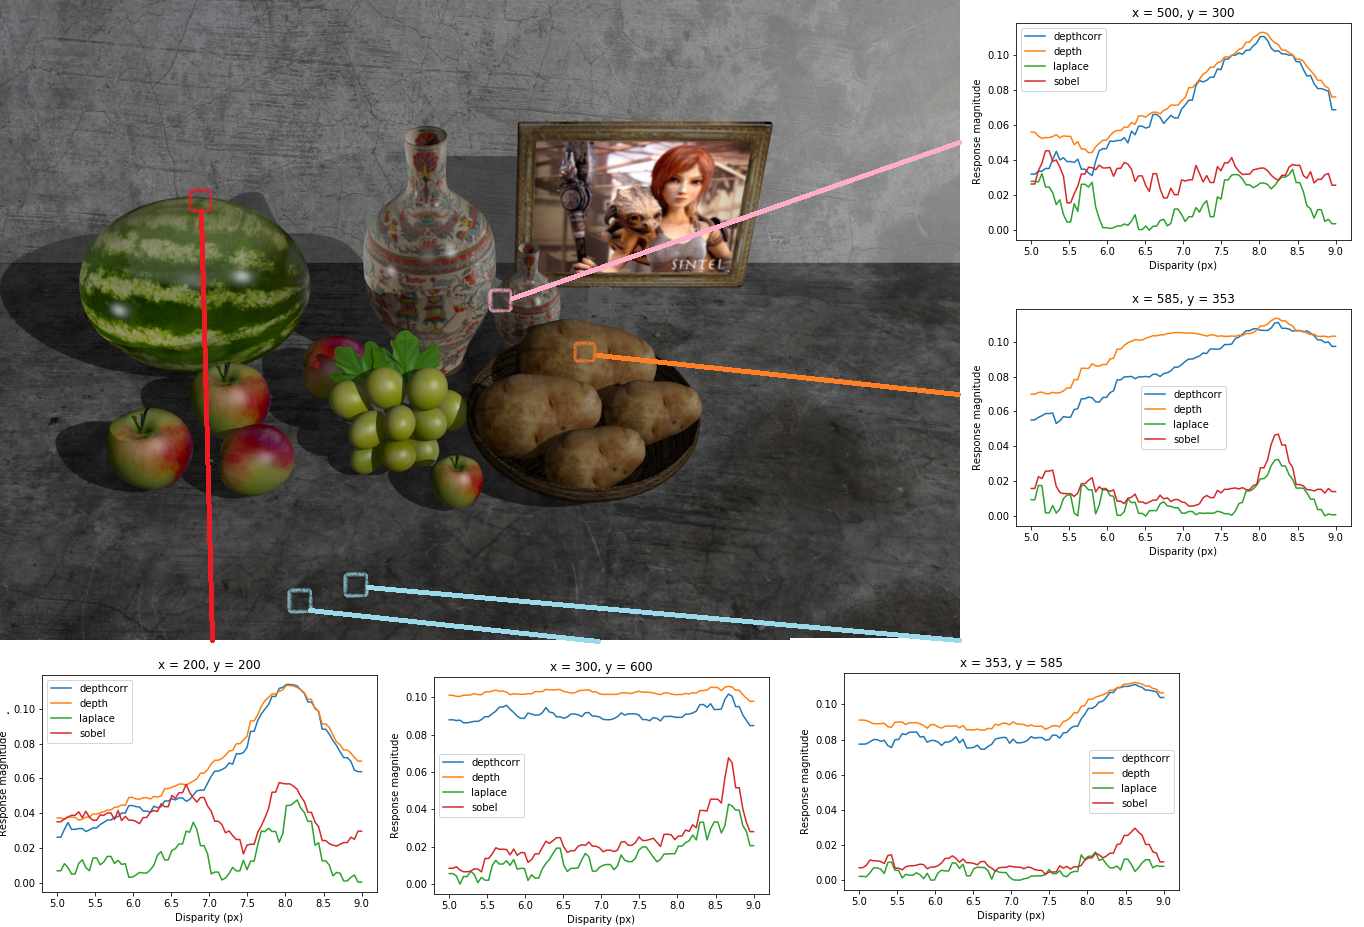
\includegraphics[width=1\linewidth]{images/original_marked}
	\caption[Pixel response for depth from focus techniques]{At different pixel positions we take a look at how the pixel response value behaves for the four different depth-from-focus techniques: Photo consistency (orange), angular correspondence (blue), first derivative (red) and the Laplace method (green). A high value means high confidence (low cost).}
	\label{fig:originalmarked}
\end{figure}
	In the following, we are going to compare the methods mentioned above qualitatively and quantitatively. In figure \ref{fig:originalmarked} one can see the pixel response value refocussed at different disparities for all the methods at example points in the test-scene \textit{complextestscene}. Points close to edges as well as points on clear surface with less structure on it are chosen. One can see that the pixel response of the angular correspondence and the photo consistency method for those points show a more consistent behaviour, meaning that only one clear maximum can be seen. The derivative method as well as the Laplace method both seem to have trouble especially on pixel coordinates close to edges. This can be seen most clearly at the edge of the melon, where the first derivative shows two maxima, while the angular correspondence and photo consistency measure find a clean maximum indicating at which depth the point can be found. However, on surfaces with less structure as for example on the potato, the photo consistency measure struggles to find a clear maximum -- still, it has the maximum at the right position.
	\begin{figure}[h!]
		\centering
		\includegraphics[width=0.8\linewidth]{images/result_depth_from_focus_res20}
		\caption[Depth from focus: Depth maps]{The depth maps of the scenes (from up to down) \textit{complextestscene, cotton, occlusiontestscene, pens, testscene, tiltplane} are depicted for different depth-from-focus techniques. The disparity step size is 1/20.}
		\label{fig:resultdepthfromfocus}
	\end{figure} 
	Having a look at the actual disparity maps produced by the different techniques (figure \ref{fig:resultdepthfromfocus}) we can already capture that the angular correspondence and photo consistency method produce the more consistent, smooth disparity maps. 
	A quantitative evaluation confirms this impression:
	The diagram in figure \ref{fig:errorres20all} shows the mean relative error for all 4 cues evaluated on the scenes depicted in figure \ref{fig:resultdepthfromfocus}. It becomes obvious that for all scenes either the photo consistency or the angular correspondence cue obtain the lowest mean relative error.	
	\begin{figure}[h!]
		\centering
		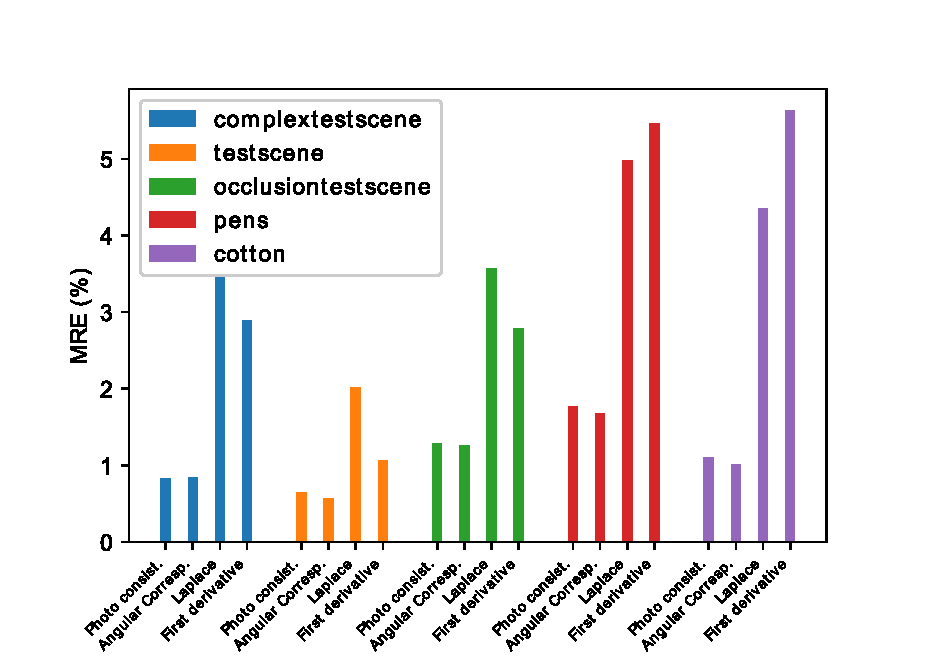
\includegraphics[width=0.7\linewidth]{images/error_res20_all}
		\caption[Mean squared error for depth-from-focus techniques]{The mean squared error is depicted for depth-from-focus techniques. The step size is 1/20.}
		\label{fig:errorres20all}
	\end{figure}
	\subsection{Using depth-from-refocus as a pre-estimate for the ST}
	\begin{figure}[h!]
		\centering
		\includegraphics[width=0.8\linewidth]{images/result_depth_from_focus_pre}
		\caption[Depth from focus: depth maps with resolution 1]{The depth maps of the scenes (from up to down) \textit{complextestscene, cotton, occlusiontestscene, pens, testscene} is depicted for different depth-from-focus techniques. On the right the ground truth is depicted. The disparity step size is 1.}
		\label{fig:resultdepthfromfocuspre}
	\end{figure}
	\begin{figure}[h!]
	\centering
	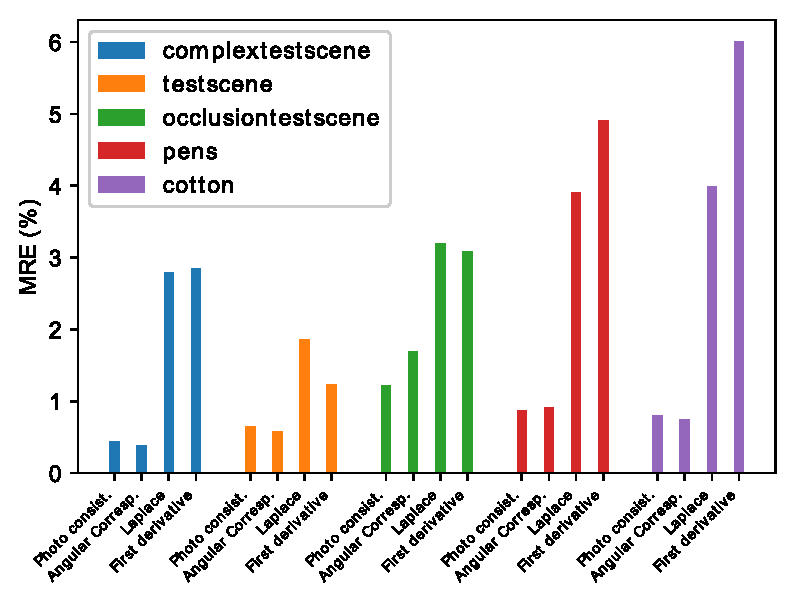
\includegraphics[width=0.7\linewidth]{images/error_res1_all}
	\caption[Mean squared error for depth-from-focus techniques]{The mean squared error is depicted for depth-from-focus techniques. The step size is 1.}
	\label{fig:errorres1all}
	\end{figure}
	 \begin{figure}[h!]
	\centering
	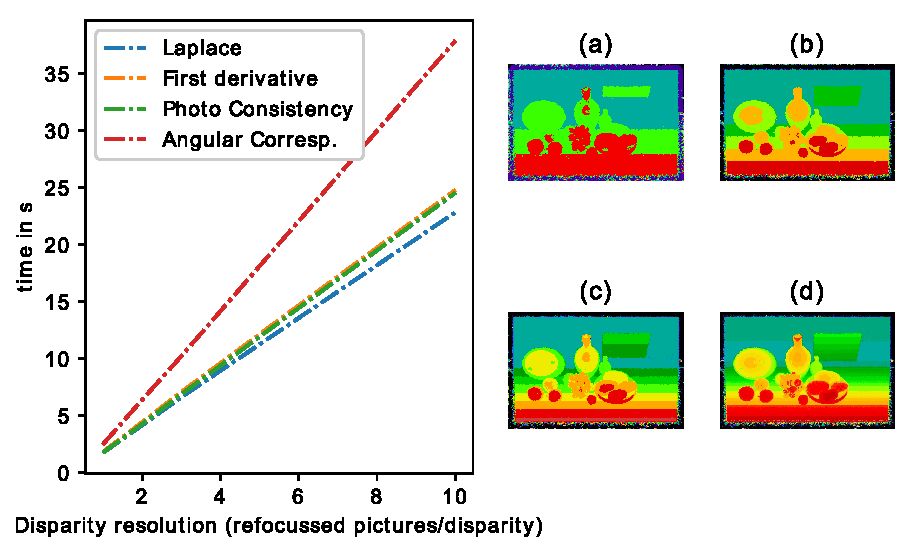
\includegraphics[width=0.7\linewidth]{images/speeds.eps}
	\caption[Speed of different depth-from-focus techniques]{ On the left, the speed of different depth-from-focus techniques is depicted in function of the resolution chosen. (a)-(d) show the disparity map of the scene \textit{complextestscene} for the resolutions 1, $\frac{1}{2}$, $\frac{1}{3}$, $\frac{1}{10}$ respectively.}
	\label{fig:speeds}
	\end{figure}
	One long-term aim of this work is to make the structure tensor pipeline more robust. We achieve this by using the depth-from-refocus method as a pre-estimate, therefore reducing the disparity window at each pixel. The light field is now refocussed by integer disparity steps, resulting in disparity maps that obtain equidistant layers. In figure \ref{fig:speeds} on the right the scene \textit{complextestscene} is shown with different refocussing stepsizes, where a) shows refocussing on integer step size.
	 All disparity maps with integer disparity step size are shown in figure \ref{fig:resultdepthfromfocuspre}, right next to the ground truth integer depth map. From the depth maps one can already guess that the angular correspondence and the photo consistency cue produce the denser depth estimates. This again is confirmed if we take a look at the MRE in figure \ref{fig:errorres1all}: The angular correspondence and photo consistency measures result in the lowest MRE, though the angular correspondence cue is about 1.5 times more time-consuming than the photo consistency measure under the same conditions. The process time for all cues is depicted in figure \ref{fig:speeds} on the left.
 	We stick to the photo consistency measure, as it produces the best results in terms of speed and precision.\\
 	The next step is to use the pre-estimate at each pixel to skip the iterative refocussing in the structure tensor pipeline. However, since not all points on an EPI are of the same depth, the EPI is segmented in parts of the same pre-estimation depth. Those parts are refocussed separately to the estimated depth, results are illustrated in figure \ref{fig:epivsgdepth}. Note that the edges of the depth images have been removed when calculating the MRE. 
 	Unfortunately, the photo consistency pre-estimate pipeline yields worse results than the ST pipeline itself. The reason is that artefacts from the pre-estimate persist after the structure tensor pipeline has been applied to the EPI.\\
 	Also, the pre-estimation is even more time-consuming than the structure tensor itself. Because of the splitting of the EPI, the runtime is scene dependent. We find significant runtime differences between the scenes, the results can be found in table \ref{tab:time_gdepth}. 
 		\begin{table}[h!]\label{tab:time_gdepth}
 		\begin{tabular}{|c|c|c|c|}
 			\hline 
 			Scene & Structure tensor pipeline & Pre-estimate+ ST & GT as pre-estimate \\ 
 			\hline 
 			\textit{complextestscene} & 12.89 s & 13.62 s & 8.83 s \\ 
 			\hline 
 			\textit{pens} & 5.1 s & 5.2 s & 4.7 s \\ 
 			\hline 
 			\textit{cotton} & 5.09 s & 6.78 s & 3.97 s \\ 
 			\hline 
 			\textit{tiltplane} & 22.25 s & 17.46 &  9.3 s \\ 
 			\hline 
 			\textit{occlusiontestscene} & 10.9 s & 12.1 s & 6.7 s \\ 
 			\hline 	
 		\end{tabular} 
 		\caption[Depth-from-focus: Time for pipelines]{Time for different pipelines. Left: We use no pre-estimate. Middle: A pre-estimation based on the photo consistency cue is used. Right: The ground truth as a pre-estimate is used.}
 	\end{table}
 	If one skips the pre-estimation step and takes the ground truth data as a 'pre-estimate', the pipeline is significantly faster than iteratively refocussing on each depth. The pre-estimation step itself takes about 2 seconds. The ST depth estimation with a depth-from-focus pre-estimation step takes longer than using the ground truth as a pre-estimation since the EPI gets segmented into more split EPIs when using the cue pre-estimate. A global smoothing scheme on the pre-estimate can possibly improve the runtime by minimizing the amount of split EPIs to be calculated, however this would result in even more artefact effects. We leave that aspect for future work.\\ In summary, we did not achieve an improvement regarding the MRE or the process time, when using the photo consistency measure as a pre-estimate for the structure tensor. 
 	\begin{figure}[h!]
 		\centering
 		\includegraphics[width=0.8\linewidth]{images/epi_vs_gdepth}
 		\caption[Photo-consistency pre-estimate for the structure tensor]{Comparison between the ST pipeline with and without a photo consistency pre-estimate. On the left, the MRE is depicted for different scenes. The right images show the absolute difference of the depth map to the ground truth, while the left column represents the results with the photo consistency pre-estimate.}
 		\label{fig:epivsgdepth}
 	\end{figure}
%\newpage
\goodbreak
\section{Modifications on the structure tensor}
\label{sec:modifications}
As depth from focus techniques didn't work out well, we examine different approaches by directly modifying the ST pipeline, with the aim of solving the occlusion problem while maintaining a dense disparity map.\\
In the following section, we concentrate on benchmark data from the dataset of \cite{honauer2016benchmark} as it not only provides a big data set, it also comes with a toolkit for evaluating scenes with different metrics. Whenever it is referred to a metric score a lower score always means better score.
\subsection{Sandglass kernel}
In figure \ref{fig:sandclockresults} the results we obtain from using a sandglass-shaped kernel instead of a normal Gaussian kernel are shown. Even though one could expect the custom-sized kernel to perform better at edges, the opposite is the case; the original Gaussian kernel outperforms the sandglass kernel in all scenes. The motivation to define the kernel in form of a sandglass was to localize structure clearly to the pixel it belongs to. However, it becomes clear that the sandglass kernel cannot handle the occlusion problem explained in section \ref{sec:occlusionproblem}. On the surface regions less smoothing between neighbouring pixels lead to a higher noise resulting in a higher mean squared error. 
\begin{figure}[h!]
	\centering
	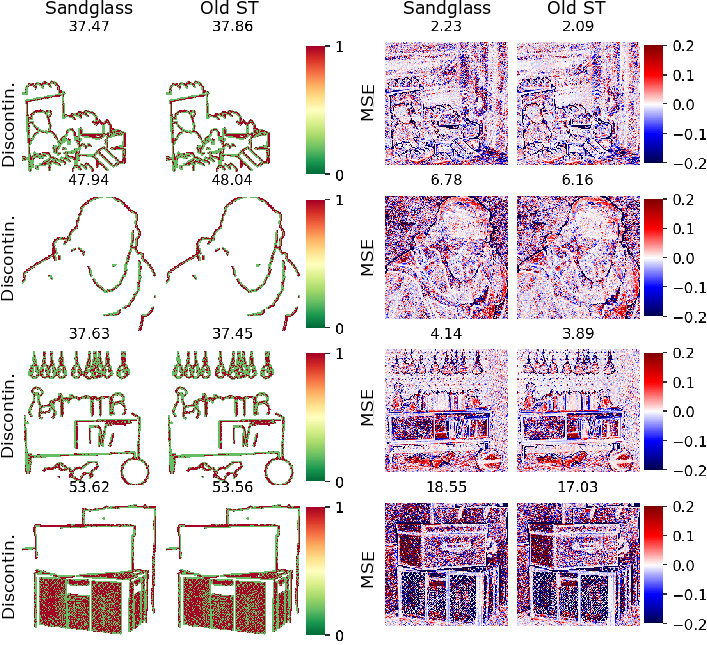
\includegraphics[width=0.7\linewidth]{images/sandclock_results}
	\caption[Results with custom sized kernel]{Comparison between the normal structure tensor and the sandglass- like kernel for the scenes \textit{dino, cotton, sideboard, boxes}. The left side compares the mean squared errors in the disparity map, the right side shows the error where discontinuities in the disparity map are masked explicitly.}
	\label{fig:sandclockresults}
\end{figure}

\subsection{Bilateral filter}
\begin{figure}[h!]
	\centering
	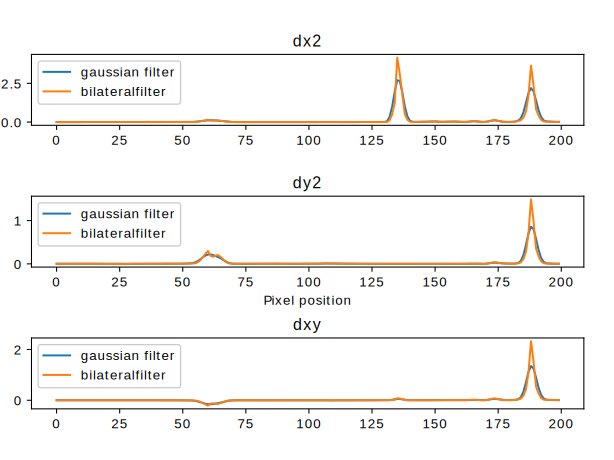
\includegraphics[width=0.7\linewidth]{images/bilat}
	\caption[Bilateral filtering]{Bilateral filtering of an EPI. Upper: EPI. Lower diagram: Structure tensor components after applying Gaussian/bilateral filter respectively.}
	\label{fig:bilat}
\end{figure}
 This section illustrates the effects of using a bilateral filter in the structure tensor pipeline instead of a Gaussian filter. Figure \ref{fig:bilateralparams} shows the MSE as well as the discontinuity score when using a bilateral filter with the original EPI as a guide.
 \begin{figure}[h!]
 	\centering
 	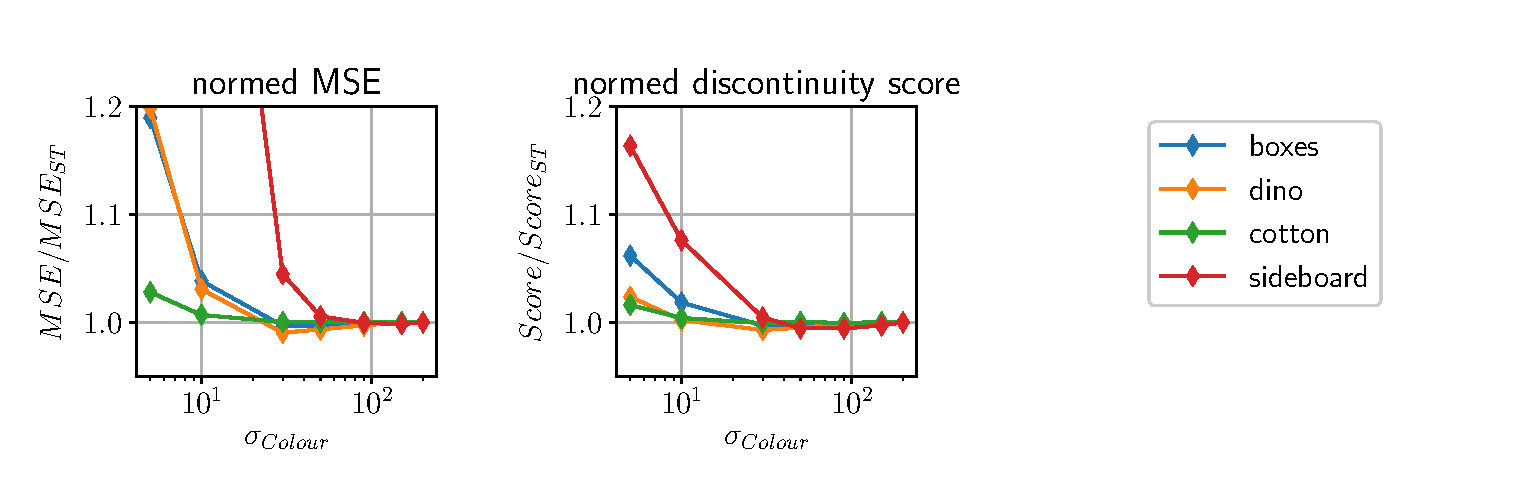
\includegraphics[width=1\linewidth]{images/bilateral_params}
 	\caption[Parameter dependency for bilateral filtering using EPI]{Bilateral filtering with original EPI as the guide: On the left, the mean squared error for different scenes in function of the $\sigma_\text{Colour}$ of the bilateral filtering is shown, divided by the MSE with using a Gaussian filter. On the right the Discontinuity score based on \cite{honauer2016benchmark} is shown, also normed to the score using the standard Gaussian filter.}
 	\label{fig:bilateralparams}
 \end{figure}
 The scores are normed to the score of the ST pipeline. For large $\sigma_\text{Colour}$ both converge to 1, because in this limit the weighting based on the colour space distance (see equation \ref{eq:bilateral}) is a constant function. Thus, one obtains the same result as with a normal Gaussian filter. Note that the $\sigma_\text{Space}$ remains the same as in the case of a normal filtering ($\sigma_\text{Space}=7$ pix). Unfortunately, the MSE metric score and the discontinuity score is worse than with using the Gaussian kernel for the complete parameter space. Especially surfaces with a lot of texture suffer from splitting the weights by their colour values. This becomes clear as the scene \textit{sideboard} with the fine patterned wallpaper reaches the worst results. Any pixel that doesn't encounter enough neighbouring pixels with an equal colour results in a  structure tensor that only takes into account the very local gradient in the EPI, resulting in a noisy disparity estimation.\\
  Since the aim was to especially handle disparity transitions by not mixing up two regions in the EPI with different colours, we take a look at the results for the discontinuity metric defined by \cite{honauer2016benchmark}. Even if one can see a slight improvement at some transitions looking at the disparity maps, the discontinuity score is unaffected since the edge fattening is still visible. It becomes visible in figure \ref{fig:bilat} that the structure tensor components along the EPI do not improve significantly using a bilateral filter due to the pre-smoothing in the ST pipeline. One would expect sharp peaks in the structure tensor components near disparity discontinuities. Since the results do not satisfy the expectation and the guided bilateral filter also takes about 5 times longer than the normal structure tensor, we try an alternative approach.\\
 Instead of using the original EPI as a guide, one could directly take the structure tensor component vector 
 \begin{equation}\label{key}
 \vec S = \left(\begin{matrix}
 \frac{\partial g^2}{\partial x \partial x} \\
 \frac{\partial g^2}{\partial s \partial s} \\
 \frac{\partial g^2}{\partial x \partial s} \\
 \end{matrix}\right)
 \end{equation}
 as the guide for the bilateral filtering of itself. The idea behind it is closely related to the EPI segmentation as described in section \ref{sec:occlusionawareness}. Big gradients in the EPI are more consistently referring to the same transition. By separating small and big gradients, the influence of the structure in front is less significant than it is without using the bilateral filtering. As one can see in figure \ref{fig:bilateralnormparams}, using the ST components as a guide can actually result in a better MSE. 
 \begin{figure}[h!]
 	\centering
 	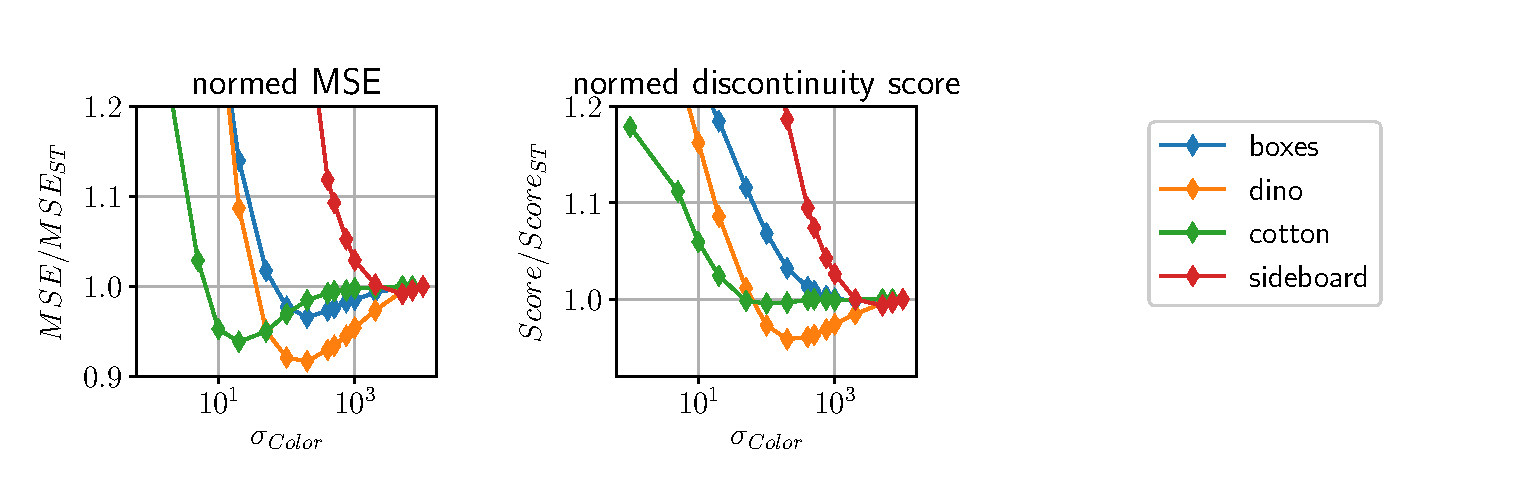
\includegraphics[width=1\linewidth]{images/bilateral_norm_params}
 	\caption[Parameter dependency for bilateral filtering]{Bilateral filtering with structure tensor components themselves as the guide: On the left, the mean squared error for different scenes in function of the $\sigma_\text{Colour}$ of the bilateral filtering is shown, divided by the MSE with using a Gaussian filter. On the right the discontinuity score based on \cite{honauer2016benchmark} is shown, also normed to the score using the standard Gaussian filter.}
 	\label{fig:bilateralnormparams}
 \end{figure}
 For each scene, the score is dependent on the parameter $\sigma$ that is chosen. Also, the discontinuity score does not improve even though in figure \ref{fig:bilatresults} a clear improvement can be seen at occlusion borders.
 \begin{figure}[h!]
 	\centering
 	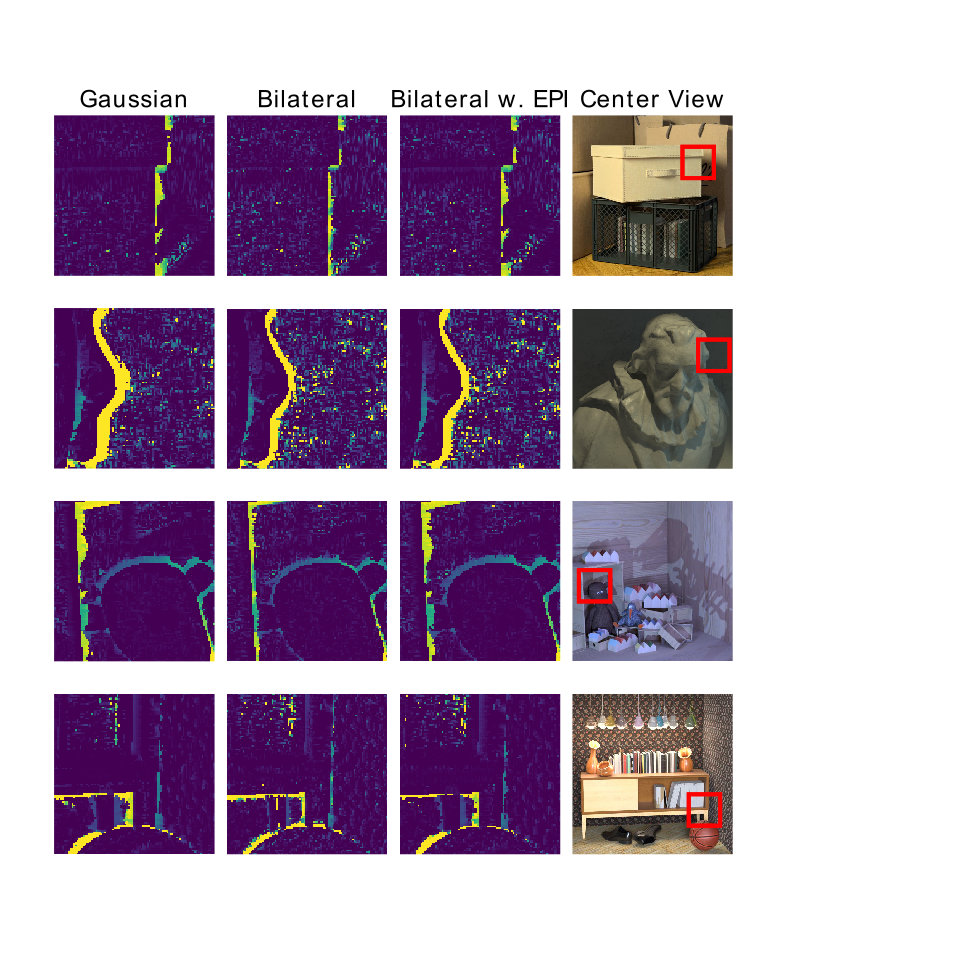
\includegraphics[width=0.7\linewidth]{images/bilat_results}
 	\caption[Results of the bilateral filtering]{Results of Bilateral filtering for the scenes \textit{ boxes, cotton, dino, sideboard}.}
 	\label{fig:bilatresults}
 \end{figure}
 Actually, the edge fattening is by far bigger than the masks used to determine the discontinuity score in figure \ref{fig:bilateralnormparams}. In figure \ref{fig:bilatresults} The depth maps zoomed at some disparity transitions in the given scenes \textit{boxes, cotton, dino} and \textit{sideboard} are shown, calculated with the Gaussian and bilateral filter. One can observe that the bilateral filter (with the structure tensor component as a guide) results in sharper edges that are significantly less 'fattened' than the Gaussian equivalent. This becomes clear when looking at the head of the teddy bear in the scene \textit{dino}. Even though the front object still occupies more space than it should (edge fattening), the edge has become smaller. This effect cannot be seen when using a bilateral filter with the EPI as a guide, however.\\
 Additionally, it becomes clear when looking at the scene \textit{boxes} in figure \ref{fig:bilatresults} that the depth estimation using the bilateral filter with the structure tensor component as a guide is less affected by the colour differences in the image. When using the Gaussian ST, the error along the edge is dependent on the background structure as the transition to the lettering on the bag results in less error than above. The bilateral filter, however, does produce a consistent error that may be better to handle for post-processing.
\subsection{Thresholding gradients}
\label{sec:ev_thresh}
\begin{figure}[h!]
	\centering
	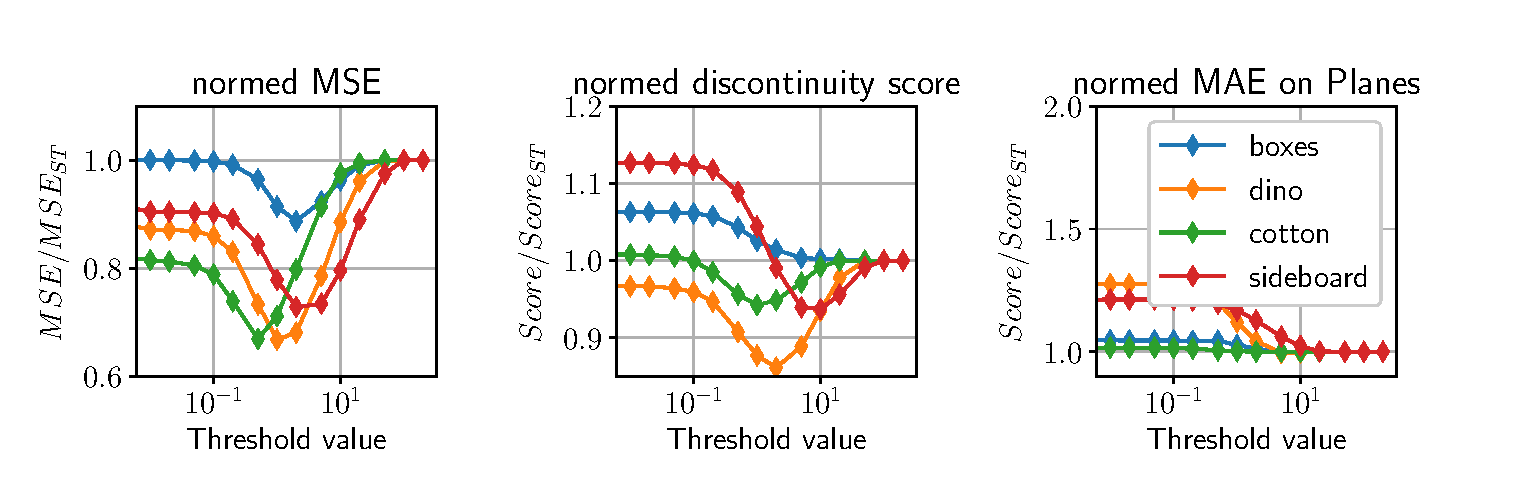
\includegraphics[width=1\linewidth]{images/thresh_params}
	\caption[Results when thresholding the gradients in the EPI]{Results when thresholding the gradients in the EPI are shown. All results are divided by the score obtained from the normal structure tensor algorithm. On the left, the MSE is shown, in the middle the discontinuity score is shown, on the right we see the MSE on planar surfaces in the scene. All metric scores follow the metrics from \cite{honauer2016benchmark}. }
	\label{fig:threshparams}
\end{figure}
When the gradient norm is thresholded as explained in section \ref{sec:thresholdinggradients}, the main aim is to change the weights of the gradients contributing to the structure tensor such that all gradients contribute the same. The smallest gradients underlay noise effects, therefore they are not upscaled. A truncation threshold is set so that all gradients in the EPI with a norm bigger than the threshold are normed to that threshold value. As one can see in figure \ref{fig:threshparams}, for big threshold values the result is equal to the old ST pipeline results as all gradients in the EPI are below the threshold, thus they are unaffected.
Setting an extremely low threshold has the same effect as normalizing all gradients to the same strength. Especially on planar surfaces which typically have less texture and therefore low gradient strengths in the EPI, the error score is worse when normalizing the gradient, as one can see in figure \ref{fig:threshparams} in the right plot. However, the MSE is mostly affected by the edge fattening error as described in section \ref{sec:occlusionproblem}. Therefore, simple normalizing already improves the MSE, since the gradient strength of the transition weights less into the structure tensor.
\begin{figure}[h!]
	\centering
	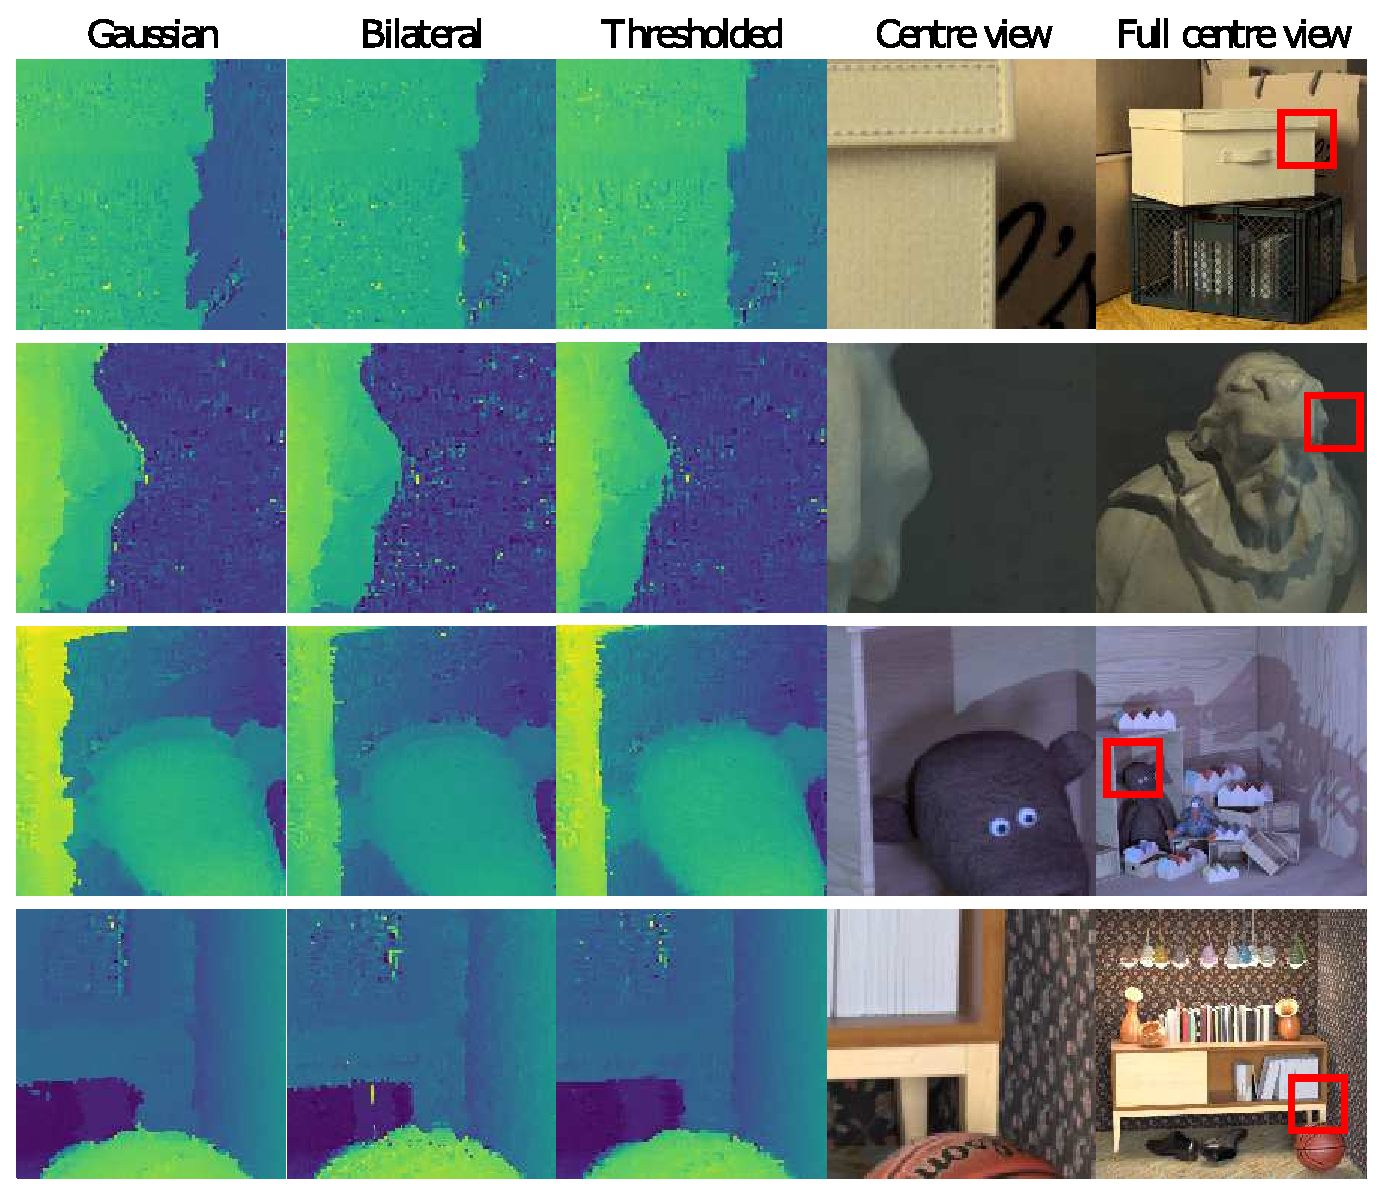
\includegraphics[width=0.7\linewidth]{images/thresh_results}
	\caption[Disparity map zoom-ins for different methods]{Disparity map zoom-ins for different ST modifications. From left to right: Gaussian filtering, bilateral filtering and Gaussian filtering when thresholding the gradients.}
	\label{fig:threshresults}
\end{figure}
Even though a low threshold improves the behaviour at discontinuities, the larger noise results in a worse BadPixel score, thus also affecting the discontinuity score. For this reason, no significant improvement can be seen in figure \ref{fig:threshresults} in the middle.
Since the scene \textit{boxes} is the noisiest one, the MSE is affected least by improving the disparity transitions. The MSE in the scene \textit{cotton} on the other hand is mostly affected by the edge fattening error, thus its MSE is improved most by the thresholding of the gradients. All scenes show an improved MSE for the complete parameter space. Note that the threshold is plotted in a logarithmic scale. In figure \ref{fig:threshresults} the thresholded gradient ST result is compared to the bilateral and Gaussian ST result. It is obvious that with a Gaussian kernel, transitions are fattened and erroneous. It seems that the bilateral filter at least for the upper 3 scenes performs best, while the thresholded ST still produces the same errors as the Gaussian ST, as one can see in the \textit{boxes}-scene (upper row). Nevertheless, the additional noise (see scene \textit{sideboard}, last row) produced by the bilateral filtering finally results in a worse MSE score. 
\begin{figure}[h!]
	\centering
	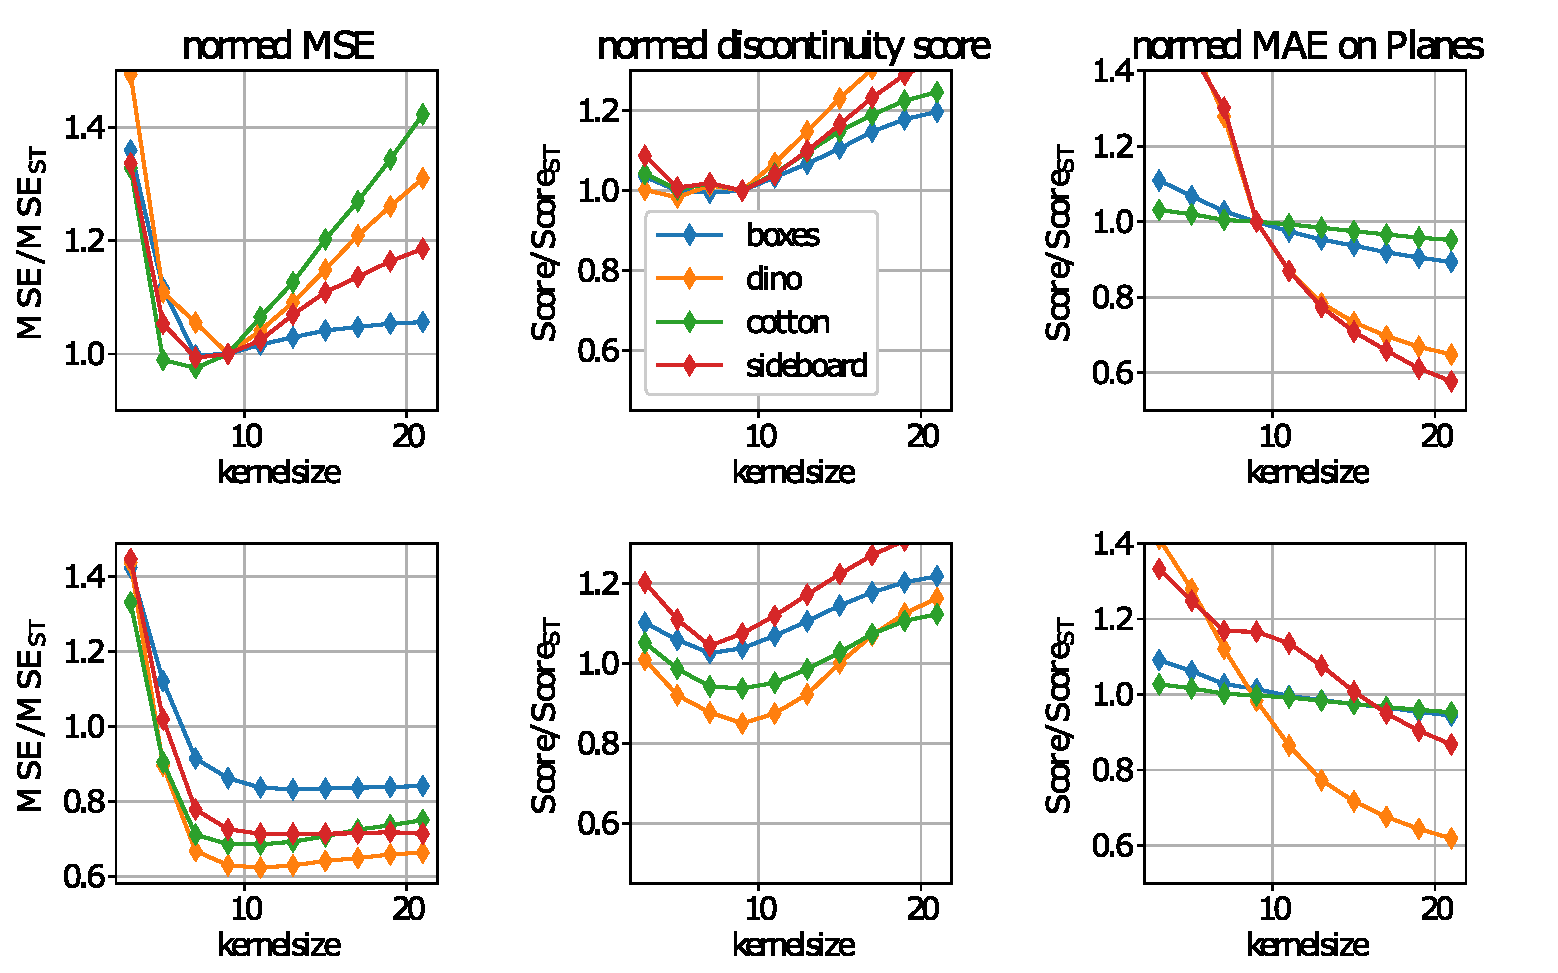
\includegraphics[width=0.8\linewidth]{images/old_outer}
	\caption[Varying kernel size]{Top:Varying the kernel size, using the old ST pipeline. Bottom: Varying the kernel size with thresholding the gradients.}
	\label{fig:oldouter}
\end{figure}
In figure \ref{fig:oldouter} the Gaussian outer kernel size is varied for the old ST and for the thresholded gradient ST. Obviously, the discontinuity score becomes worse for bigger gradients and the error score on planes improves due to bigger kernels being less affected by noise in both cases. In contrast to the old ST pipeline, the MSE stays constant for large kernel sizes.
\subsection{Occlusion awareness segmentation}
\label{sec:occlusionawareness}
In the next step we are trying to detect occlusions in the scan directly via the gradient norm since a high gradient is a good indicator for an occlusion edge (explained in section \ref{sec:occlusionsegmentation}). The result, though, is dependent on multiple parameters, two of them are the kernel size of the morphology closing kernel.
\begin{figure}[h!]
	\centering
	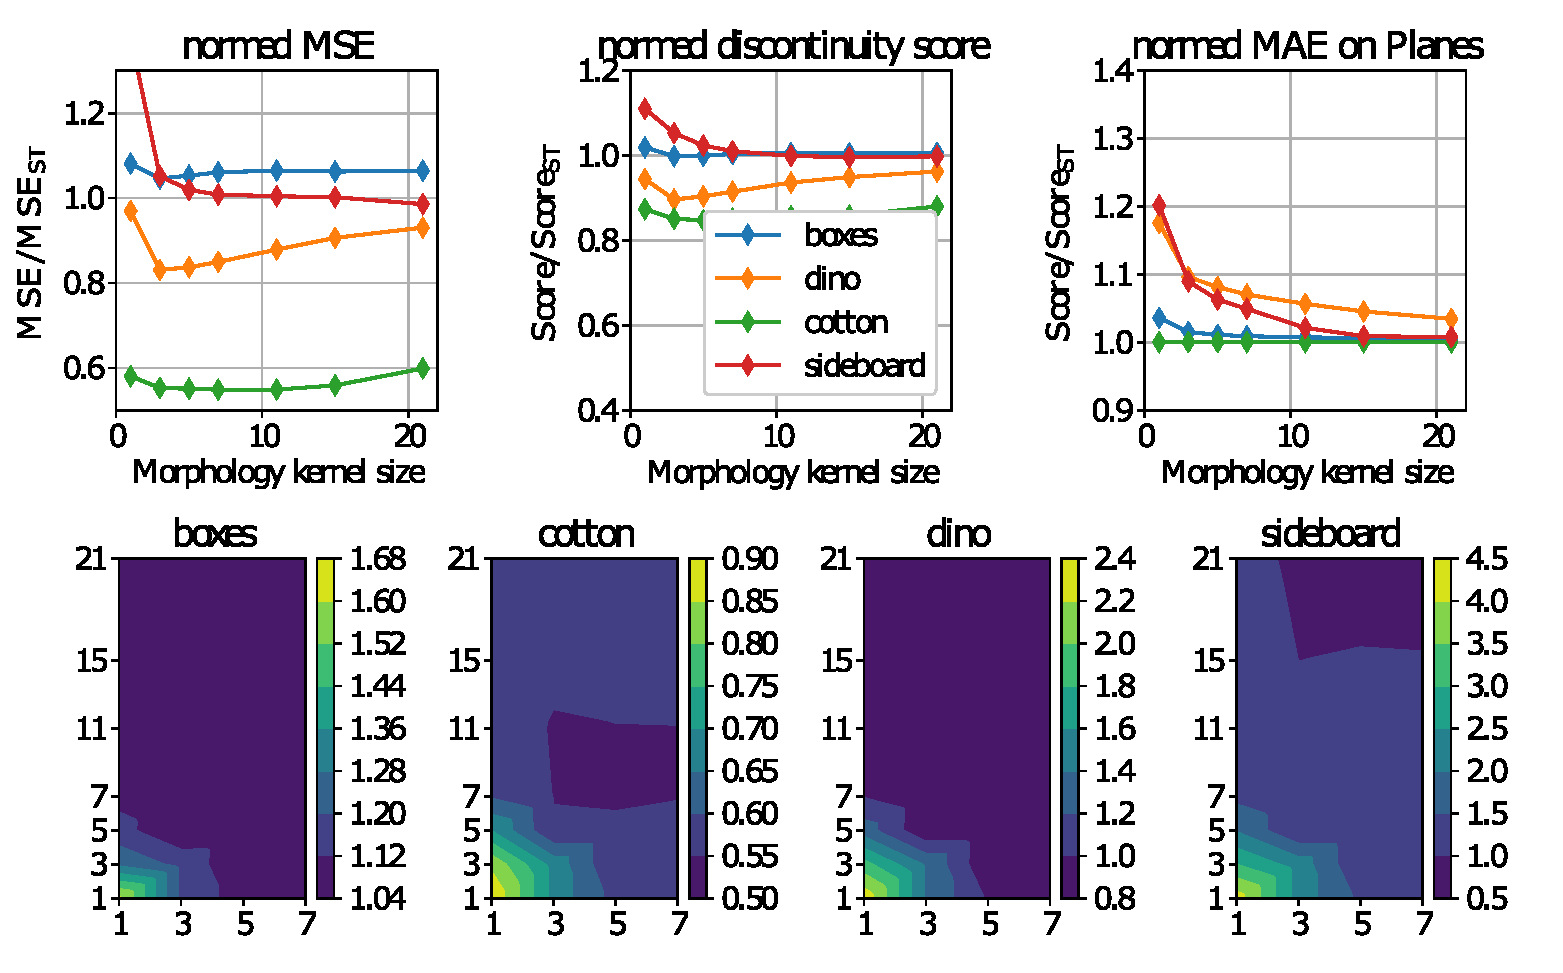
\includegraphics[width=0.8\linewidth]{images/thresh_segm_morph}
	\caption[Segmentation of EPI dependence on the morphology kernel]{Upper row: Metric scores in dependence of the size in y-direction of the morphology kernel, x-direction size is 7.\\ Lower row: dependence of the MSE for the size of the kernel. the y-size is depicted on the x-axis.}
	\label{fig:threshsegmmorph}
\end{figure}
In figure \ref{fig:threshsegmmorph} (upper row) the metric scores are plotted in function of the y-directional size of the kernel. The x-morphology kernel is held constant to the size of 7. From figure \ref{fig:threshsegmmorph} (lower row) we can extract, that for all scenes we obtain the best result when sticking to a 7-pix x-directional kernel size. As the EPI is only 9 pixels wide, we do not use larger kernels.\\
The larger the kernel size is, the larger the connected parts belonging to the same segment in the EPI are. More segmentations have a negative effect on the mean average error on planar surfaces with lots of texture, which we can see in the scenes \textit{dino} and \textit{sideboard}. This is confirmed in the upper right plot showing the MAE on planar surfaces for bigger and smaller closing kernels. A larger morphology size kernel results in a better planar surface score, however in the limit for very large kernels no segmentation is happening, thus the relative score is converging to 1. Furthermore, the scenes \textit{cotton} and \textit{dino} are the ones whose mean squared error is mostly dependent on occlusions in the scene.
\begin{figure}[h!]
	\centering
	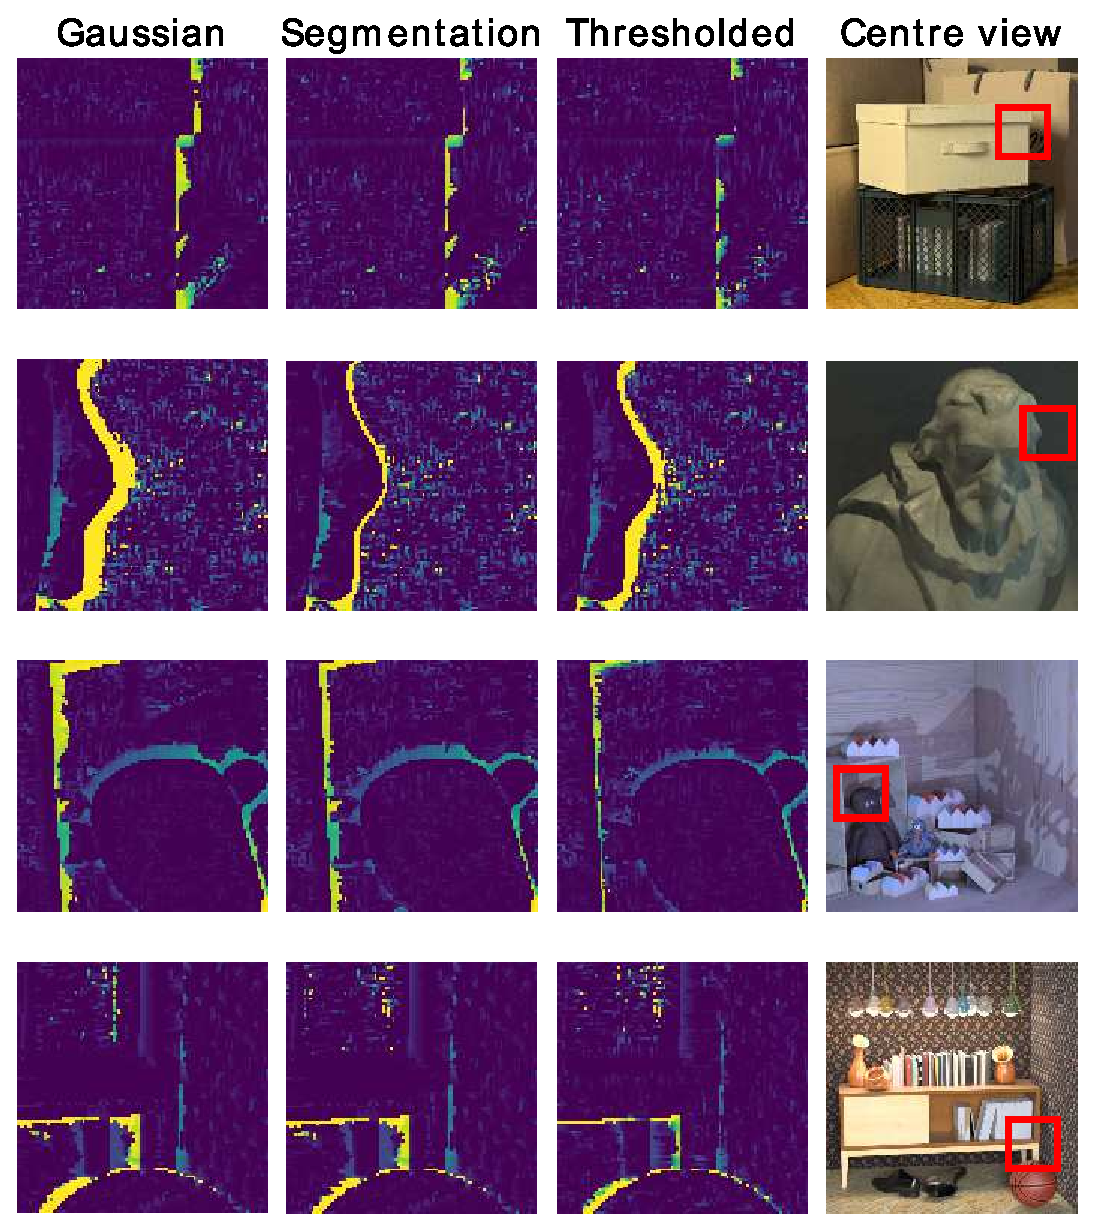
\includegraphics[width=0.8\linewidth]{images/thresh_results_morph}
	\caption[Disparity map zoom-ins for different methods]{Disparity map zoom-ins for different structure tensor filtering. From left to right: Gaussian filtering, segmentation filtering and Gaussian filtering with thresholding the gradients.}
	\label{fig:threshresultsmorph}
\end{figure}
In figure \ref{fig:threshresultsmorph} the segmentation algorithm is compared to the old pipeline as well as to the thresholded norm pipeline that is evaluated in the previous section. Again we have a look at the same scenes \textit{boxes, cotton, dino} and \textit{sideboard}. It becomes clear that both algorithms to some degree improve the depth reconstruction near occlusion edges. Still, the results differ from each other. In the zoom-in on the scene \textit{boxes} the thresholded pipeline seems to achieve slightly better results, however on the occlusion in the scene \textit{cotton} the segmentation algorithm proves to produce better results. The segmentation especially works well with 'clean' edges, where the edge itself results in a clear peak in the norm of the plot (See figure \ref{fig:derivativesfull} in section \ref{sec:occlusionsegmentation}). In the other scenes, however, the segmentation does not seem to work well as the algorithm only achieves minor improvements.
\subsection{Alternative coherence}
\label{sec:alternative_ev}
\begin{figure}[h!]
	\centering
	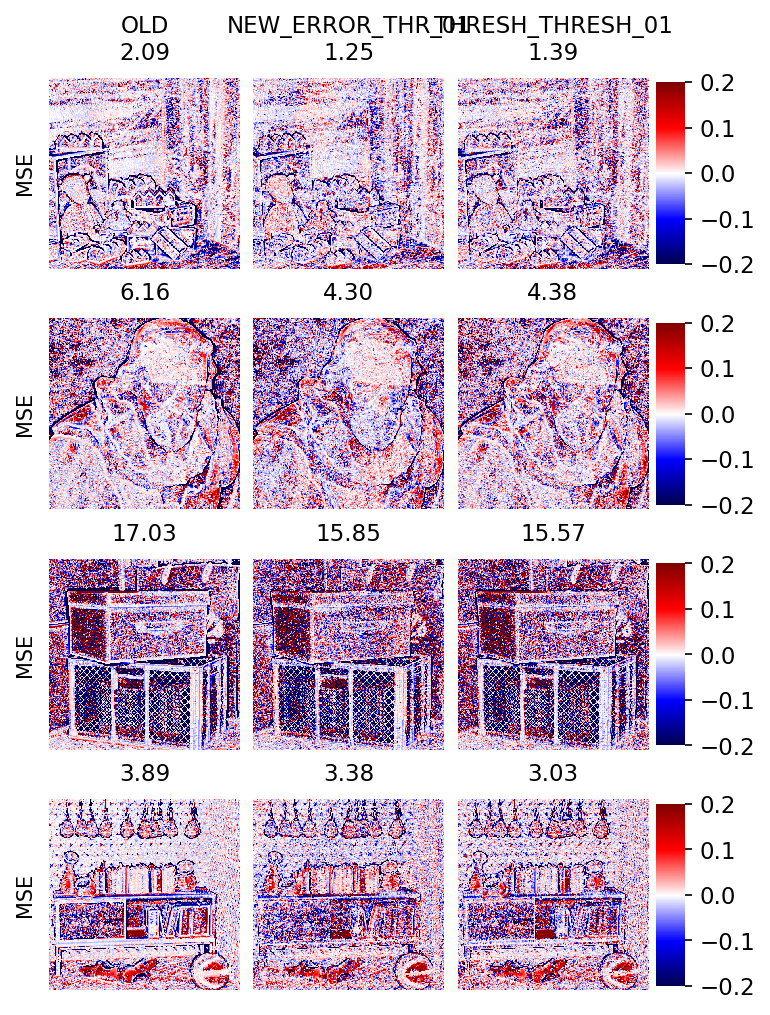
\includegraphics[width=0.7\linewidth]{images/thresh_vs_old_vs_newerror}
	\caption[Comparing alternative coherence to new coherence]{Left: The mean squared error using the old ST pipeline. Middle: Using the alternative error measure + thresholding the gradients. Right: Using the old coherence measure + thresholding the gradients.}
	\label{fig:threshvsoldvsnewerror}
\end{figure}
The use of the alternative cost function as explained in section \ref{sec:alternative} only works in combination with thresholding the gradient (section \ref{sec:thresholdinggradients}). For this reason, we compare the error maps of the old pipeline, the threshold pipeline and the new error measure to each other in figure \ref{fig:threshvsoldvsnewerror}.
From the given score above each sub-image, one can conclude that the new error measure does perform about equally as good as the thresholded pipeline. The alternative coherence measure was expected to result in a better disparity map because in theory, it should handle occlusion edges to some degree better than the old coherence measure does. Still, \ref{fig:threshvsoldvsnewerror} shows that the errors remain roughly in the same spots.
\begin{figure}[h!]
	\centering
	\includegraphics[width=0.8\linewidth]{images/old_vs_alternative}
	\caption[Old coherence vs new error]{Columns on the left: The coherence value from the horizontal EPI, vertical EPI and the merged coherence map. Middle to the right columns: Alternative error measure based on error propagation. On the very right: Actual deviation from the ground truth.}
	\label{fig:oldvsalternative}
\end{figure}
Both the old coherence and the new error measure calculate the respective error from the EPI in horizontal and vertical direction. Both views get merged based on the error measure of each view, resulting in a merged coherence/error map. This can be seen in figure \ref{fig:oldvsalternative}, where for each scene the horizontal, vertical and merged coherence/error map is illustrated as well as the actual error that was produced by the pipeline.
Since in figure \ref{fig:threshvsoldvsnewerror} one recognizes that the disparity error maps for both pipelines don't differ much, only the error of the old pipeline is shown in figure \ref{fig:oldvsalternative}. One can see that the merged error of the new error measure seems to have a bigger overlap with the actual error, making it a better tool for masking out bad pixels than the coherence value. Especially in the scene \textit{cotton} the occlusion edge errors fit better to the error with the new error measure.\\
To quantify this result, we choose different error thresholds for both pipelines and set all disparity values whose related error is below the threshold to zero. The higher the amount of masked out pixels is, the higher we expect the MSE to be since the number of disparity values being 0 increases linearly (those disparity values also account for the total MSE). This linear relation between the percentage of disparity values set to zero and the total MSE is plotted in figure \ref{fig:newerrorconfidence} in a logarithmic manner.
\begin{figure}[h!]
	\centering
	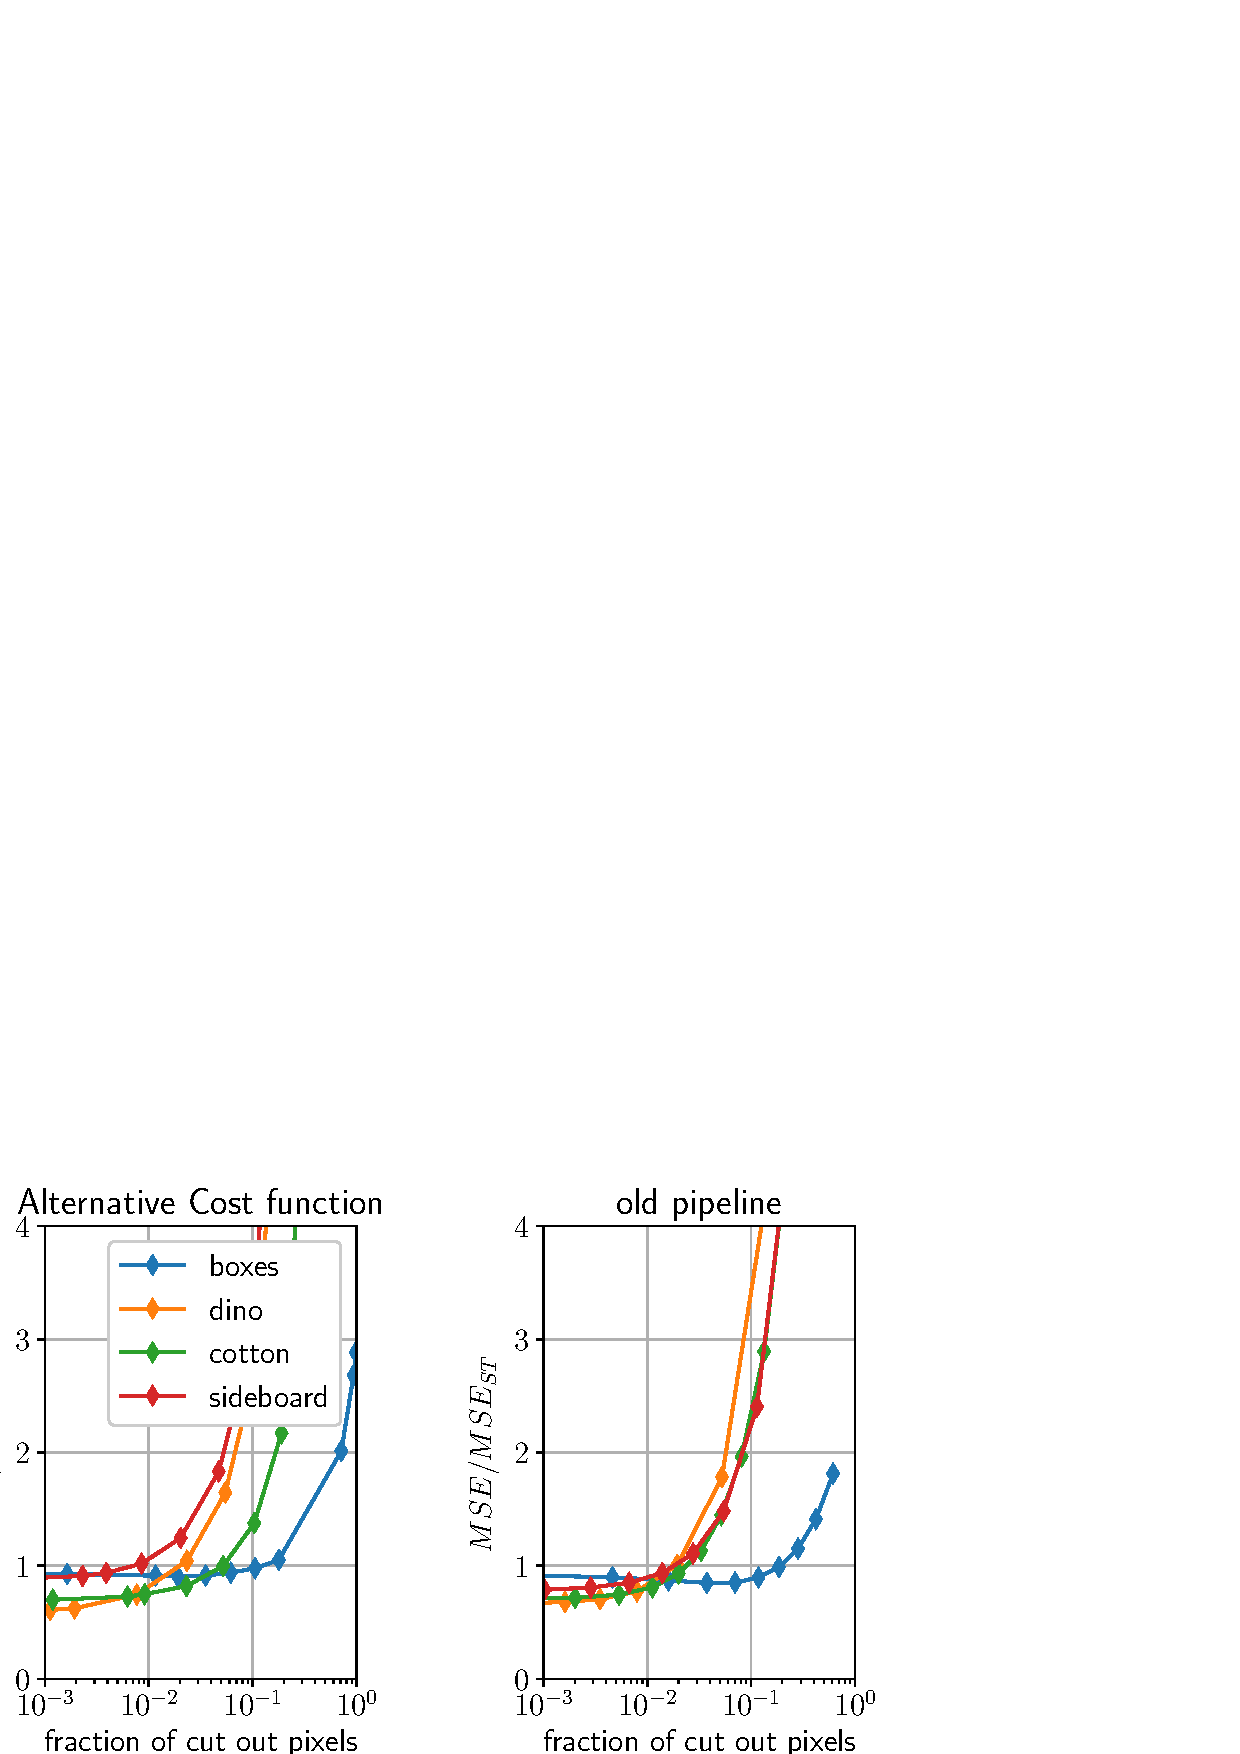
\includegraphics[width=1\linewidth]{images/newerror_confidence}
	\caption[Dependence of error on cut out pixels]{The relative MSE is plotted against the percentage of pixels that are set to 0 at different coherence values. On the left, the new error metric is used. On the right, the old pipeline is used.}
	\label{fig:newerrorconfidence}
\end{figure}
Using equal axes this would result in curves with linear form. The logarithmic scale, however, allows us to evaluate more easily how many pixels have to be set to zero until the result gets significantly worse. As long as the masked out pixels are already highly inaccurate, the resulting MSE doesn't change much by setting them to zero. These plots confirm the observation that the error in the scene \textit{cotton} is prognosticated better by the new error measure, since setting the upper 10 $\%$ of the highest error pixels to 0 results in a better score than doing the same with the old coherence measure. In the other scenes, the quality of the error measure is around equal in both cases. In the appendix we show a visualization of the quality of the depth maps using histograms (section \ref{sec:alternative_app}).
\subsection{Alternative merging of x- and y-direction}
\label{sec:ev_merging}
When merging the x- and y- directional depth estimations giving preference to the depth value that is further away, one obtains better results on occlusion edges while the number of outliers rises. This trade-off is favourable, as long as the noisy outliers can be handled by post-processing algorithms. The trade-off is controlled via the threshold in equation \ref{eq:altmerging} and is set to 0.7 in figure \ref{fig:chooselowerresults}. 
\begin{figure}[h!]
	\centering
	\includegraphics[width=0.7\linewidth]{images/choose_lower_results}
	\caption[Results from alternative merging of x- and y- direction]{Left columns: Comparison between the old merging and the new merging for the whole depth map. The absolute deviation from the ground truth is shown. Middle columns: Close-up view on occlusion edges. Right column: Localisation of the close-up view in the scene. Parameter from equation \ref{eq:altmerging} is set to 0.7.}
	\label{fig:chooselowerresults}
\end{figure}
In the close-up views of the deviation from the ground truth in all four scenes (column 3 and 4 in figure \ref{fig:chooselowerresults}) one sees that occlusion edges are significantly improved, especially in scene \textit{boxes} and \textit{dino}. In scene \textit{cotton} the edge remains, however it is smaller. The last scene does not show a significant improvement at occlusions. In all scenes the noise has increased. While on occlusions the coherence does not serve as a good measure to decide whether to take the x-directional or the y- directional depth estimation, on planar areas a higher coherence value is mostly the better one. As a result, one faces noise as it can be observed well in scene \textit{boxes} and \textit{sideboard}. \\
Nevertheless, the MSE is improved for all scenes if the threshold value is set between 0 and 0.5 as one can see from figure \ref{fig:chooselowerparams} on the left side.
\begin{figure}[h!]
	\centering
	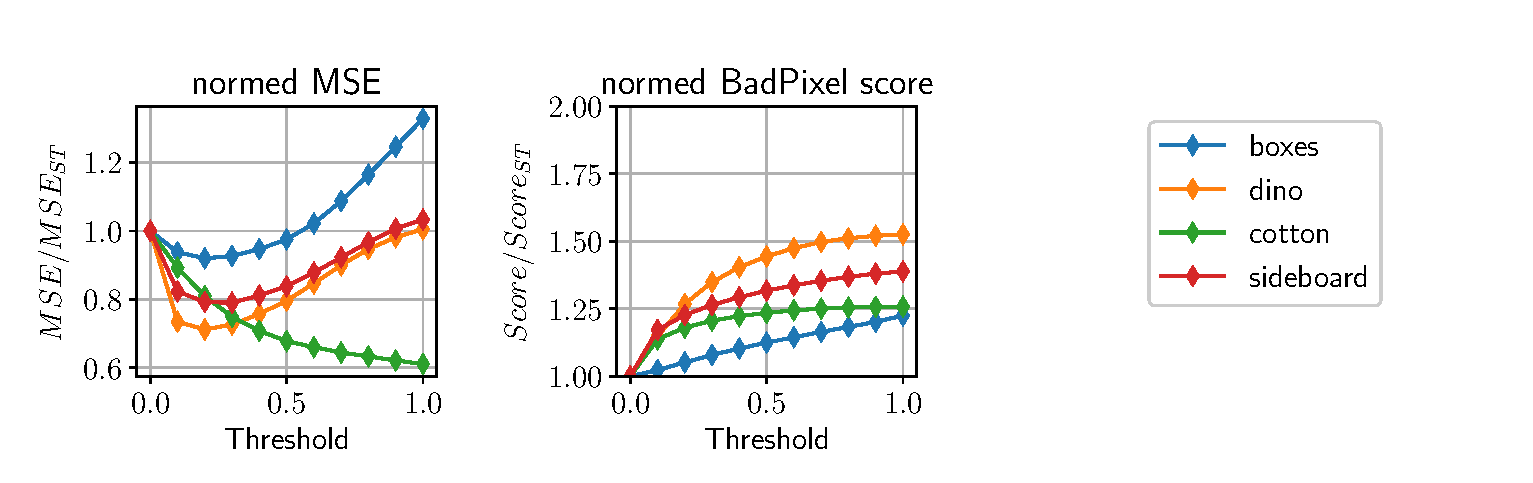
\includegraphics[width=1\linewidth]{images/choose_lower_params}
	\caption[Alternative merging: Parameter dependence]{Alternative merging: Parameter dependence. Left: Mean squared error. Right: BadPixel score.}
	\label{fig:chooselowerparams}
\end{figure}
The threshold value 0 corresponds to the old pipeline, the threshold value 1 corresponds to always choosing the lower disparity value. Choosing big threshold values leads to increased noise, thus worsening the MSE score. Note that we can see from figure \ref{fig:chooselowerparams} on the right that the BadPixel score is increasing, followingly the amount of pixels that are highly accurate decreases for a high threshold value. However, the occlusion handling can compensate for the noise which is leading to the increased BadPixel score. Further, we can smoothen out slight errors more easily than bigger deviations at occlusion edges.
\begin{figure}[h!]
	\centering
	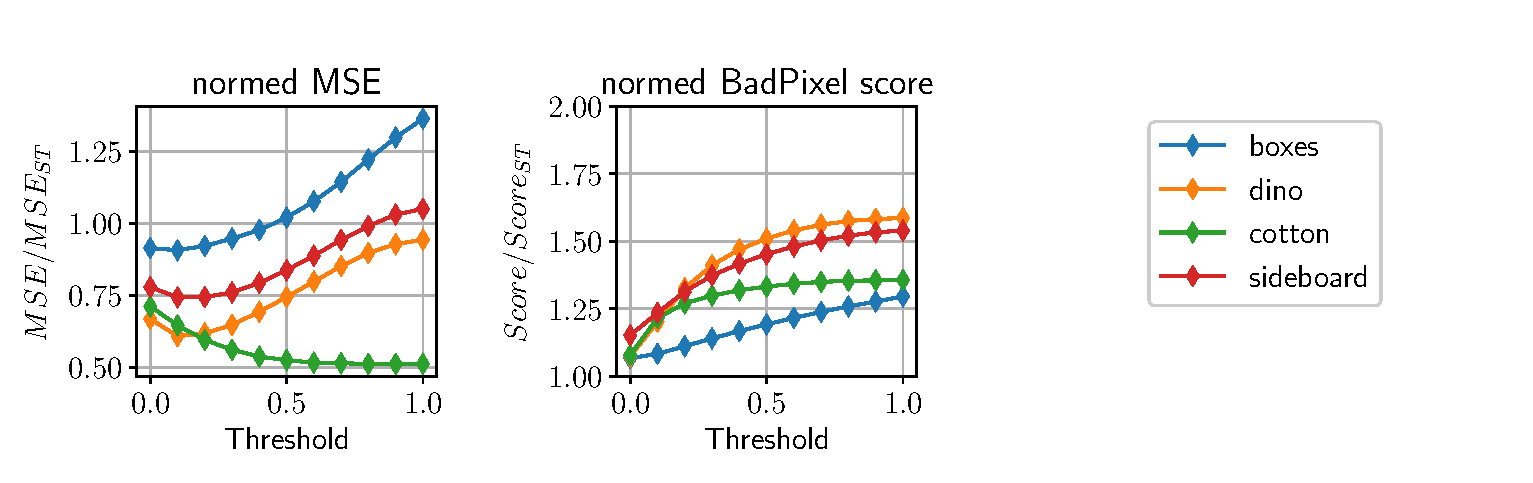
\includegraphics[width=1\linewidth]{images/choose_lower_params_thresh}
	\caption[Alternative merging: Parameter dependence]{Alternative merging + thresholded gradients: Parameter dependence. Left: Mean squared error. Right: BadPixel score.}
	\label{fig:chooselowerparamsthresh}
\end{figure}
The same plot can be found in figure \ref{fig:chooselowerparamsthresh} where the algorithm is combined with thresholding the gradients as described in section \ref{sec:thresholdinggradients}. One can see that we can see a slight improvement in the MSE for the scenes \textit{dino} and \textit{sideboard}, while the improvement of the occlusions in scene \textit{boxes} cannot compensate the increasing noise. The scene \textit{cotton} with big occlusion edges obtains the best result for the highest threshold value. Even though it doesn't improve the MSE score it may be favourable to have this merging implemented if it can be handled by post-processing smoothing. This is evaluated using the SGM algorithm in section \ref{sec:sgmppr_ev}. Note that the dependent parameter is the one referenced in equation \ref{eq:altmerging}, the gradient threshold is set to 0.1 . For this reason, the $MSE/MSE_{ST}$ score does not start at 1. Even though in figure \ref{fig:chooselowerparams} and figure \ref{fig:chooselowerresults} it seems that occlusions can be handled by alternative merging, the gradient threshold does the same, such that both combined do not necessarily improve the result as seen in figure \ref{fig:chooselowerparamsthresh} on the left. For a higher merging parameter, the BadPixel score is always increasing due to the higher noise coming from low coherence disparity values.
\section{Semi-global matching}
\label{sec:sgm}
\subsection{In-process SGM}
First, we evaluate the SGM algorithm as described in section \ref{sec:semiglobal3}. The disparity candidates as well as the related cost values are obtained from the structure tensor estimate on the EPI at different disparity shifts.
The SGM algorithm as implemented here is dependent on 3 parameters as implemented  from equation \ref{eq:global_sgm_cont_occlusion}.
 \begin{figure}[h!]
	\centering
	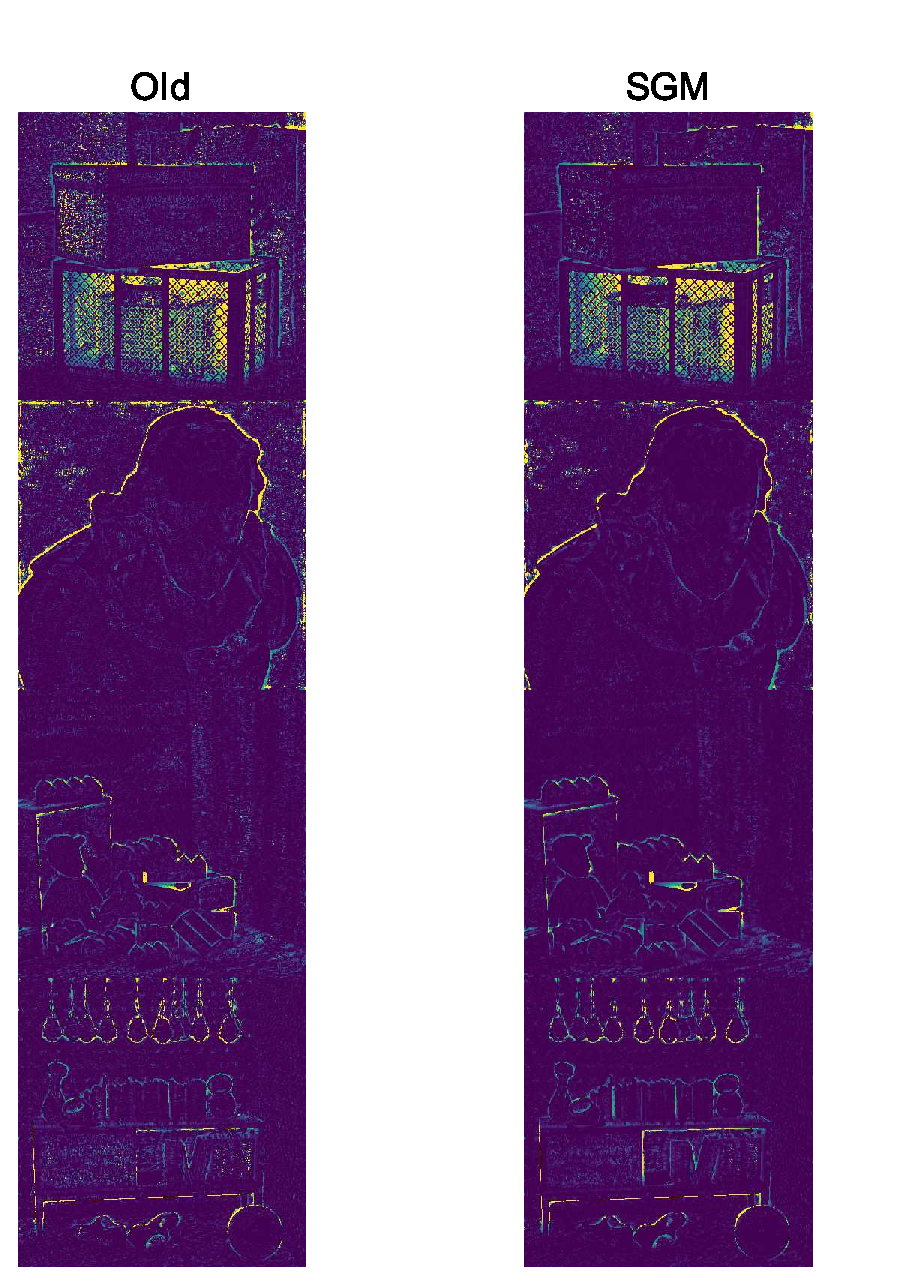
\includegraphics[width=0.7\linewidth]{images/sgm_results_thresh}
	\caption[Semi-global matching results]{Disparity error maps using the old pipeline (left) and the SGM algorithm (right). Yellow is a big deviation, dark-purple is no deviation.}
	\label{fig:sgmresultsthresh}
\end{figure}
We tried to perform a grid search to find the best parameters. The illustration of the grid search can be found in the appendix in figure \ref{fig:sgmparamscontourmse100}, \ref{fig:sgmparamscontourdis} and \ref{fig:sgmparamscontourdmae} for different metrics. The difference between the maximum and minimum score in the grid search is too small to see any clear dependence on any of the parameters. Note that we sampled the parameter space logarithmically to cover a wider space. Obtaining independence of the parameters is positive for working with the algorithm, the reason for the independence lies in the fact that at most pixels the candidate disparity values between which the SGM algorithm decides are the same. If the structure tensor only finds one unambiguous disparity value, this value is chosen regardless of the parameters.
On planar surfaces this unambiguity is not given, thus the SGM algorithm is able to smoothen such surfaces. This can be seen in figure \ref{fig:sgmresultsthresh}, where the old pipeline is compared to the result using the SGM algorithm. The depth map is improved at surfaces with noisy values, thus the SGM has a smoothing effect. At occlusion edges the SGM pipeline does not perform significantly better. 
\subsection{Improved coherence measure by using SGM}
\label{sec:improved_coh}
Even though the SGM pipeline does not handle occlusion edges well, it still does recognize disparity jumps as high costs in the cost function. In figure \ref{fig:sgmcoherencethresh} the cost function is depicted in comparison to the actual error as well as in comparison to the old pipeline. Large disparity jumps are punished with a big penalty, thus they can be detected easily. In scene \textit{cotton} and \textit{sideboard} such disparity jumps are detected, while the other disparity jumps we see are less than one pixel shift and they are only punished by a small penalty. The cost function itself could be used to mask out possibly erroneous pixels.
However, the usability of an error measure based on SGM is restricted due to the dependence on the penalty parameters mentioned in equation \ref{eq:global_sgm_cont_occlusion}.
\begin{figure}[h!]
	\centering
	\includegraphics[width=0.7\linewidth]{images/sgm_coherence_thresh}
	\caption[SGM Coherence measure]{The assumed error (grey-valued) when calculating depth without using SGM (left) and with SGM (right). In Colour the actual deviation from ground truth for both pipelines is depicted. Yellow is a big deviation, dark-purple is no deviation.}
	\label{fig:sgmcoherencethresh}
\end{figure}
\subsection{SGM as pure post-processing}
\label{sec:sgmppr_ev}
For now, we take as input the processed disparity map from the structure tensor and create the SGM candidates at each pixel from the local neighbourhood as described in section \ref{sec:postprocessing_smoothing}.
\begin{figure}[h!]
	\centering
	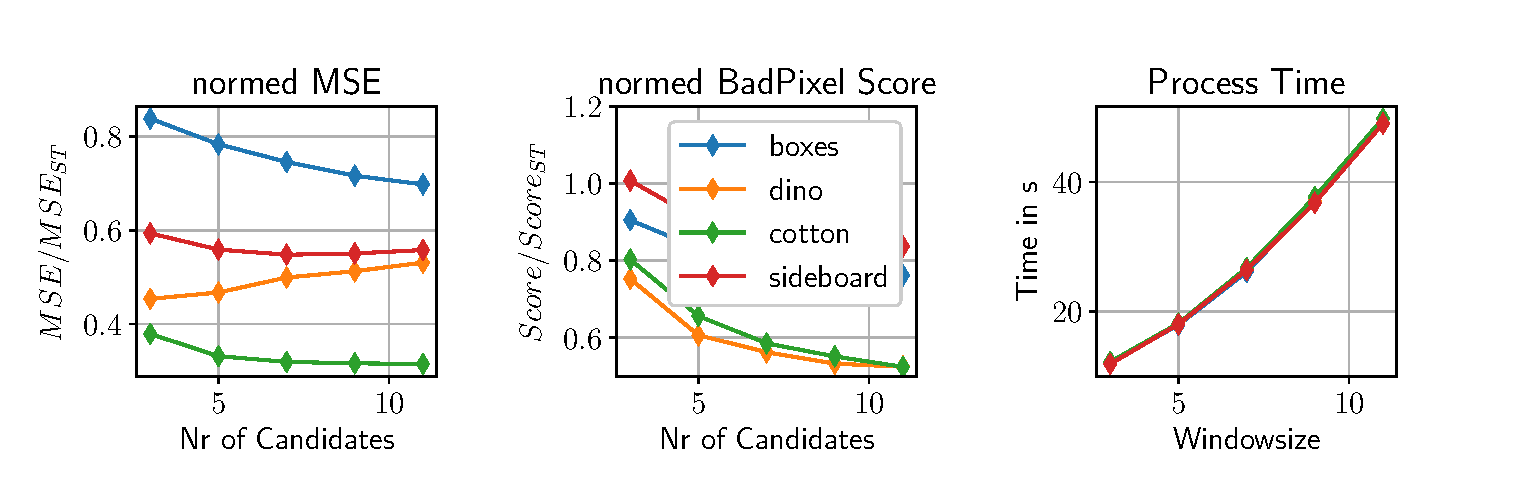
\includegraphics[width=01\linewidth]{images/choose_lower_sgm_ppr_windowsize_5}
	\caption[SGM as pure post-processing combined with alternative merging parameter dependence]{SGM as pure post-processing combined with alternative merging: The number of candidates that is chosen from the direct neighbourhood is varied. Left/Middle: The MSE/BadPixel score in dependence of the Nr of candidates. Right: the processing time of the algorithm dependent on the Nr of candidates. The window size is held constant at 5.}
	\label{fig:chooselowersgmpprwindowsize5}
\end{figure}
Figure \ref{fig:chooselowersgmpprwindowsize5} shows how MSE, BadPixel score and processing time depend on the number of candidates from the local neighbourhood which is defined as a 5x5 window around the relevant pixel. The candidates are chosen randomly from the neighbourhood. Note that the input depth map has been created with a modified structure tensor pipeline including thresholded gradients and alternative merging. The gradient threshold is constantly set to 0.1, while the merging parameter is set to 0.3 .\\
One sees that the MSE not necessarily improves given more candidates. In the scene \textit{cotton} and \textit{sideboard} we reach a fast saturation of the MSE while in the scene \textit{boxes} one would even need more candidates to reach convergence. This has to do with the large noisy regions in the scene that make it impossible to get an acceptable candidate from the neighbourhood. In scene \textit{dino} the MSE even gets worse with a higher number of candidates. On the other hand, the BadPixel score is improved for all scenes. One can conclude that the post-processing SGM manages to improve the depth map at small regions of deviations (outliers), however larger erroneous regions cannot be corrected because of the limited amount of candidate values. Using an iterative approach we try to overcome this problem in the next section.\\ 
Since the SGM algorithm is implemented here as a pure post-processing step, one can analyse the effect of applying modifications on the structure tensor beforehand. Figure \ref{fig:chooselowersgmppr} shows the dependence on the merging parameter that is characterized by equation \ref{eq:altmerging}. 
\begin{figure}[h!]
	\centering
	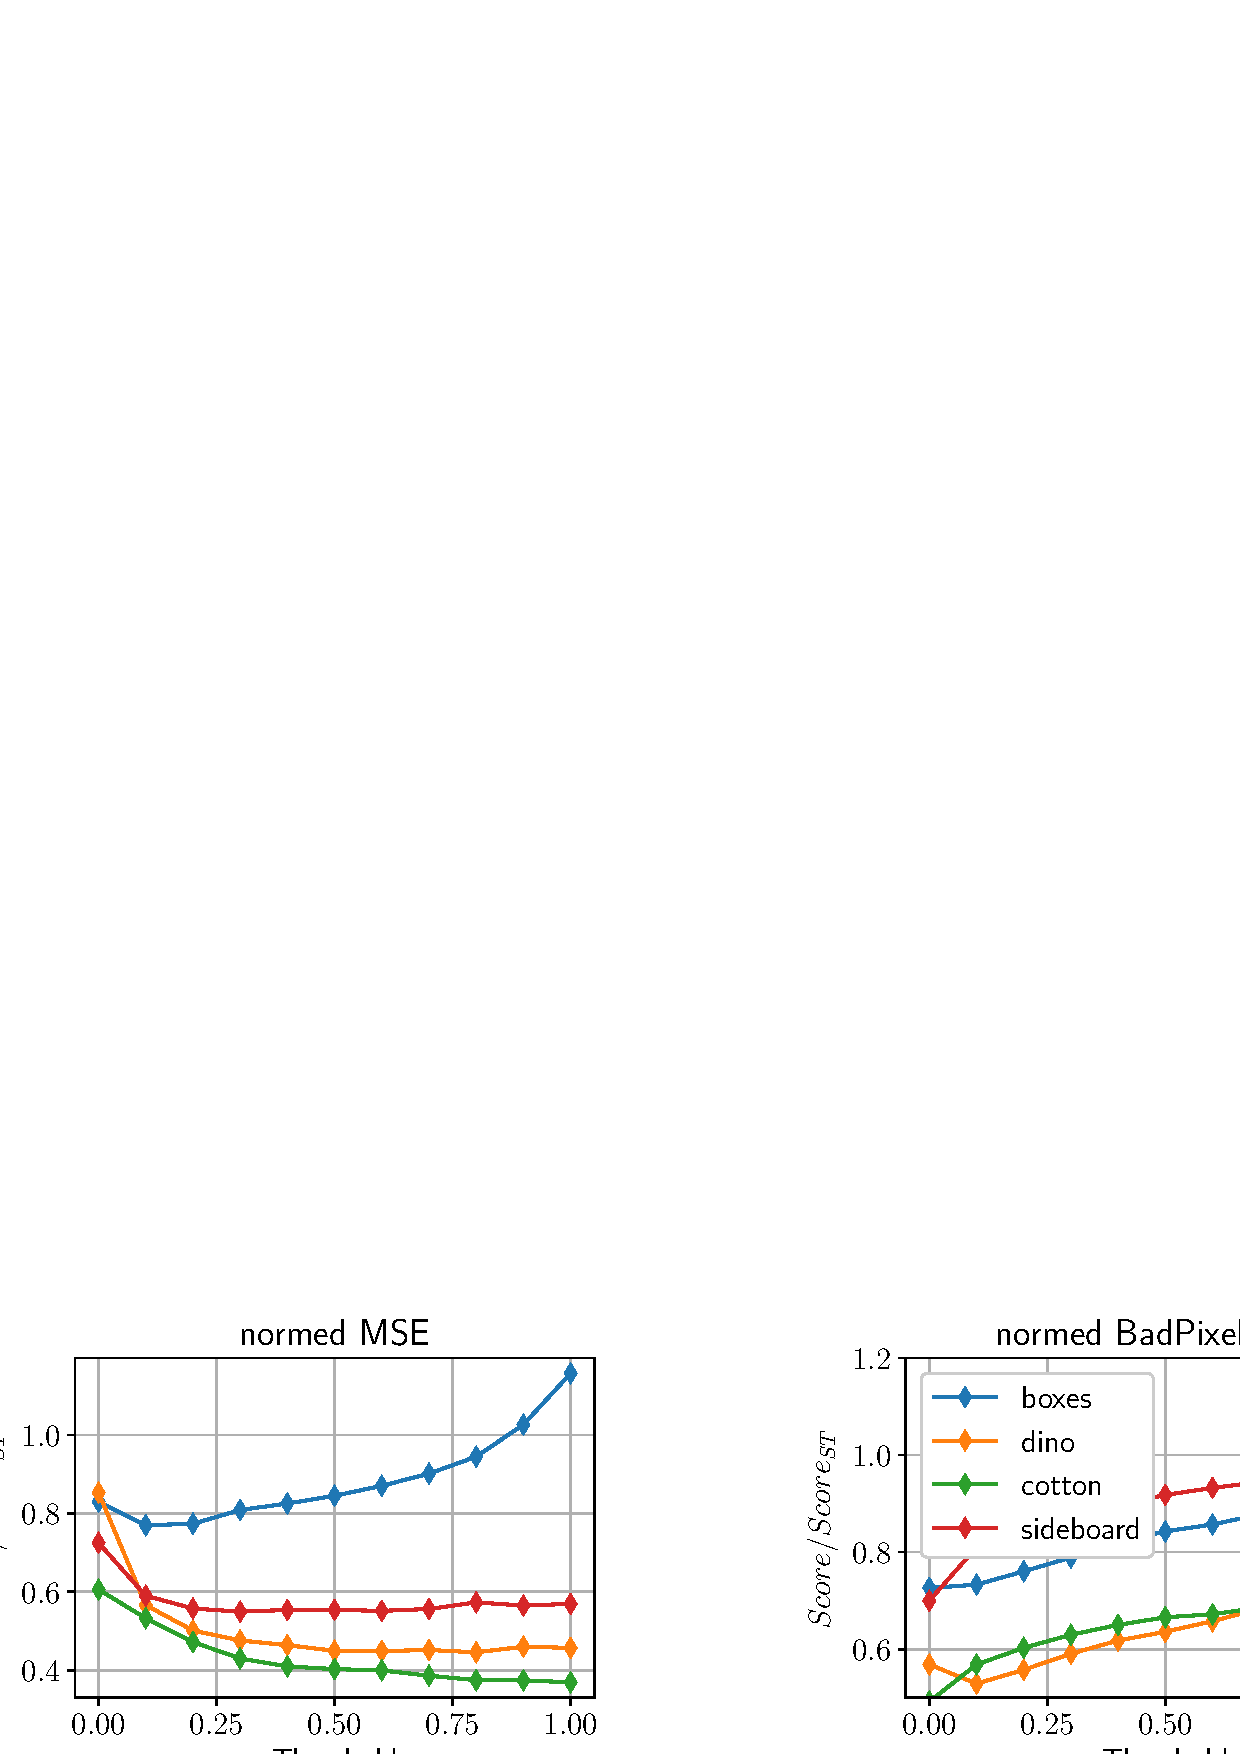
\includegraphics[width=1\linewidth]{images/choose_lower_sgm_ppr}
	\caption[Alternative merging with SGM post-processing]{Alternative merging with SGM post-processing Left/Right: MSE/BadPixel score as a function of the merging threshold.}
	\label{fig:chooselowersgmppr}
\end{figure}
No thresholding of the gradient is applied here. Larger parameters lead to better results at discontinuities, however as already shown in section \ref{sec:ev_merging} a higher merging parameter leads to an increased BadPixel score, though the normed score stays below the 1.0 mark. Again scene \textit{boxes} reaches a high MSE due to the large monochrome areas leading to noisy depth maps. One solution to handling such large deviations at surfaces is to mask out contiguous regions of low coherence. This has been implemented for the application on real data, see section \ref{sec:realdata}.\\
As we did before in section \ref{sec:ev_merging} we now take a look at the effect of implementing a gradient threshold additionally. In Figure \ref{fig:chooselowersgmpprthresh} the MSE and the BadPixel score are shown in dependence of the merging parameter.
\begin{figure}[h!]
	\centering
	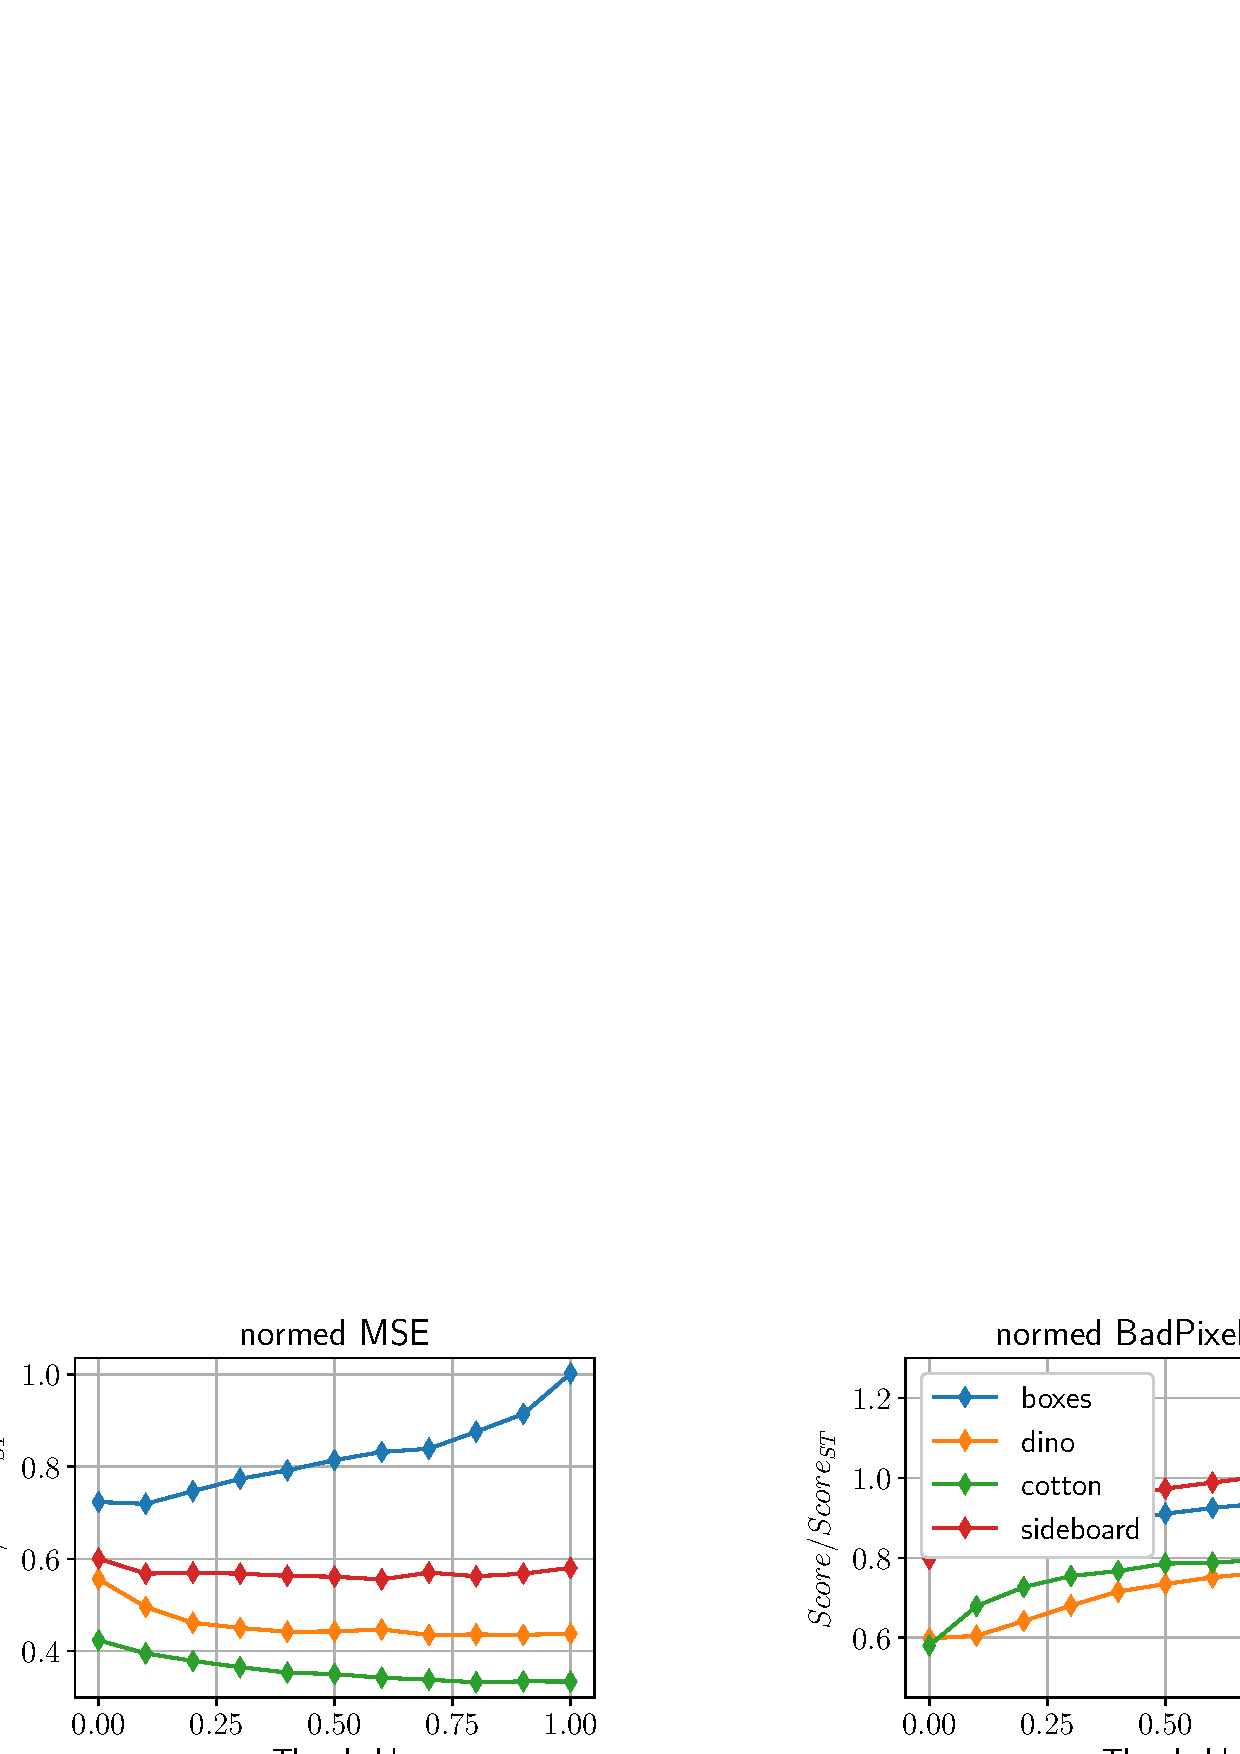
\includegraphics[width=1\linewidth]{images/choose_lower_sgm_ppr_thresh}
	\caption[Alternative merging with SGM post-processing with thresholded gradients]{Alternative merging with SGM post-processing while using thresholded gradients. Left/Right: MSE/BadPixel score as a function of the merging threshold.}
	\label{fig:chooselowersgmpprthresh}
\end{figure}
While the BadPixel score behaves approximately as without a gradient threshold (figure \ref{fig:chooselowersgmppr}), the MSE stays approximately constant for all scenes besides scene \textit{boxes}. No big improvement can be obtained since the thresholding of the gradients already handles occlusions well. 
In figure \ref{fig:chooselowersgmppr} as well as in figure \ref{fig:chooselowersgmpprthresh} the MSE does not rise for a larger merging parameter as it does in figure \ref{fig:chooselowerparams} and in \ref{fig:chooselowerparamsthresh}, where no SGM has been applied. The SGM can handle the noisy effects which occur for a high merging parameter.
\ \\
Using a grid search we tried to investigate the impact of varying the Nr of candidates as well as the window size on different metrics. In figure \ref{fig:chooselowersgmpprcontourmse100} the MSE is shown in dependence of Nr of candidates and window size for all four scenes, in figure \ref{fig:chooselowersgmpprcontourbadpix_0070} the BadPixel score is shown and in \ref{fig:chooselowersgmpprcontourbadpixel_discontinuities0070} the Discontinuity score is depicted. It becomes clear that the ideal kernel size varies strongly from scene to scene as well as from metric to metric. Based on the shown results we fix the window size to 5x5 pixels. In general a higher number of candidates promises better results. However, the processing time scales linearly with the number of candidates. Thus we stick to a number of candidates of 5, as shown in figure \ref{fig:chooselowersgmpprwindowsize5} on the right.
\begin{figure}[h!]
	\centering
	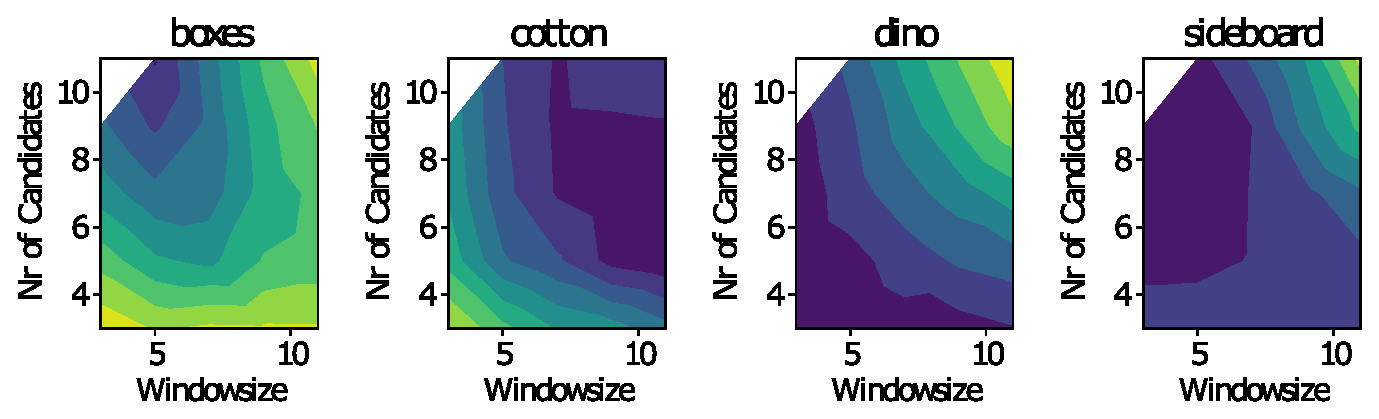
\includegraphics[width=1\linewidth]{images/choose_lower_sgm_ppr_contour_mse_100}
	\caption[Parameter dependence for post-processing SGM using alternative merging+thresholded gradients.]{MSE Parameter dependence for post-processing SGM using alternative merging+thresholded gradients.}
	\label{fig:chooselowersgmpprcontourmse100}
\end{figure}

\begin{figure}[h!]
	\centering
	\includegraphics[width=1\linewidth]{images/choose_lower_sgm_ppr_contour_badpix_0070}
	\caption[BadPixel parameter dependence for post-processing SGM using alternative merging+thresholded gradients.]{BadPixel score parameter dependence for post-processing SGM using alternative merging+thresholded gradients.}
	\label{fig:chooselowersgmpprcontourbadpix_0070}
\end{figure}

\begin{figure}[h!]
	\centering
	\includegraphics[width=1\linewidth]{images/choose_lower_sgm_ppr_contour_discontinuities_0070}
	\caption[Discontinuity score parameter dependence for post-processing SGM using alternative merging+thresholded gradients.]{Discontinuity score parameter dependence for post-processing SGM using alternative merging+thresholded gradients.}
	\label{fig:chooselowersgmpprcontourbadpixel_discontinuities0070}
\end{figure}
\subsection{Iterative SGM post-processing}
In the following, we evaluate the iterative SGM post-processing as described in section \ref{sec:iterative}. The iterative optimization should lead to a minimization of the global cost function. The global cost function is defined as the mean cost value at all pixels. In figure \ref{fig:iterationcostcotton} we confirm the iterative convergence of the mean cost function on the example scene \textit{cotton}.
\begin{figure}[h!]
	\centering
	\includegraphics[width=1\linewidth]{images/iteration_cost_cotton}
	\caption[Iterative improvement of scene \textit{cotton}]{In the upper row the resulting depth map deviation from ground truth of the iterative SGM pipeline is shown for scene \textit{cotton}. Below the mean cost function averaged over all pixels as well as the MSE is depicted in dependence of the number of iterations. Note that the MSE is not normed as in figure \ref{fig:chooselowersgmpprmergeiterations}.}
	\label{fig:iterationcostcotton}
\end{figure}
Parallel to the mean cost function the MSE also converges to a minimum. With the given set of parameters one can conclude that approximately 8 iterations are necessary to converge closely to the minimum value. In the upper row of figure \ref{fig:iterationcostcotton} one can see how the iterative process smoothens outliers in the depth map.\\
The effect of the number of iterations on the MSE can also be extracted from figure \ref{fig:chooselowersgmpprmergeiterations}. 
\begin{figure}[h!]
	\centering
	\includegraphics[width=1\linewidth]{images/choose_lower_sgm_ppr_merge_iterations}
	\caption[Iterative SGM dependence on number of iterations]{Iterative SGM pipeline dependence on number of iterations. Left: Normed mean squared error for all four scenes in function  of the number of iterations. Middle: Normed BadPixel score in function of the number of iterations. Right: Processing time.}
	\label{fig:chooselowersgmpprmergeiterations}
\end{figure}
On the left, the normed MSE is plotted. It becomes obvious that all scenes converge to a minimal MSE, however at different speed. Also for scene \textit{cotton} and \textit{dino} the BadPixel score drops, while for scene \text{boxes} and \textit{sideboard} it stays constant. However, the process time increases linearly with the number of iterations. Thus we stick to a maximum of 5 iterations in the upcoming calculation. This is still far from being comparable to the structure tensor pipeline; however, as mentioned in section \ref{sec:SGM_implement} we focus on the feasibility of such method and try to adapt the process time to a reasonable amount of time for our measuring purposes.
In the following, we want to examine the effects of changing the initial $\Delta$ (see section \ref{sec:iterative}) on the MSE as well as on the BadPixel score. In Figure \ref{fig:chooselowersgmppriterations5smoothingdelta} The MSE and BadPixel score are plotted in function of $\Delta_\text{initial}$.
\begin{figure}[h!]
	\centering
	\includegraphics[width=1\linewidth]{images/choose_lower_sgm_ppr_iterations_5_smoothing_delta}
	\caption[Iterative SGM dependence on initial $\Delta$ with 5 iterations]{Iterative SGM pipeline dependence on initial $\Delta$ with fixed number of iterations (5). Left: normed Mean Squared Error for all four scenes in function of $\Delta$. Middle: Normed BadPixel score in function of $\Delta$. Note that the x axis scale is logarithmic.}
	\label{fig:chooselowersgmppriterations5smoothingdelta}
\end{figure}
The iteration number is set to five. For very low as well as for high initial $\Delta$ no convergence can be reached in a reasonable amount of iterations. Doing only 5 iterations we find the ideal $\Delta_\text{initial} \approx 1$. It makes sense to choose the parameter at the same magnitude of the image disparity range to reach any disparity value.
The same plot as in figure \ref{fig:chooselowersgmppriterations5smoothingdelta} can be found in figure \ref{fig:chooselowersgmppriterations10smoothingdelta}, with a different number of iterations (10).
\begin{figure}[h!]
	\centering
	\includegraphics[width=1\linewidth]{images/choose_lower_sgm_ppr_iterations_10_smoothing_delta}
	\caption[Iterative SGM dependence on initial $\Delta$ with 10 iterations]{Same plot as figure \ref{fig:chooselowersgmppriterations5smoothingdelta}, doing 10 iterations instead of 5.}
	\label{fig:chooselowersgmppriterations10smoothingdelta}
\end{figure}
While the $MSE$ for small initial $\Delta$ doesn't change, we observe convergence for larger $\Delta$. Interestingly the overall $MSE$ minimum shifts to the right. Outliers that are distinct from their ground truth can only converge with a large number of iterations as well as a large enough $\Delta_\text{initial}$. This is now given with $\Delta_\text{initial} = 10$.
Further, we examine the effect of changing the smoothing parameter P1 from equation \ref{eq:recursive1dexp}. This parameter changes the form of penalizing disparity deviations from 2 neighbouring points on an SGM scanline. For very small P1 the penalty function is close to being a constant regardless of the disparity deviations, thus no convergence can be reached. In figure \ref{fig:chooselowersgmpprmergeiterationsexppenalty1} the MSE as function of the smoothing parameter P1 can be seen on the left.
\begin{figure}[h!]
	\centering
	\includegraphics[width=1\linewidth]{images/choose_lower_sgm_ppr_merge_iterations_exp_penalty1}
	\caption[Iterative SGM dependence on smoothing parameter]{Iterative SGM pipeline dependence on smoothing parameter P1 from equation \ref{eq:recursive1dexp} with fixed number of iterations (5). Left: Normed mean squared error for all four scenes in function of P1. Middle: Normed BadPixel score in function of P1. Note that the x-axis scale is logarithmic.}
	\label{fig:chooselowersgmpprmergeiterationsexppenalty1}
\end{figure}
In the limit of a very large parameter P1 the penalty function takes the form of a linear increase as function of the disparity difference between 2 depth values. This in general oversmoothens the edges as shown in figure \ref{fig:lineariteration}. While oversmoothing has a small impact on the MSE it does have impact on the BadPixel score. In the middle of figure \ref{fig:chooselowersgmpprmergeiterationsexppenalty1} we see that the BadPixel score reaches a minimum for a smoothing parameter of the magnitude of 1.
All scenes are plotted in figure \ref{fig:sgmresultsiterative} in comparison to the ground truth as wee as to the ST pipeline. While outliers such as in the background from scene \textit{cotton} are handled well, noisy surfaces as in scene \textit{boxes} cannot be handled. In all scenes surfaces are smoother after using SGM while edges are still maintained.
\begin{figure}[h!]
	\centering
	\includegraphics[width=0.8\linewidth]{images/sgm_results_iterative.png}
	\caption[Iterative SGM: depth maps]{Depth map of scenes \textit{boxes, cotton, dino, sideboard} from up to down. Left: Old pipeline depth map. Middle: Ground truth. Right: SGM iterative post-processing.}
	\label{fig:sgmresultsiterative}
\end{figure}
\newpage
\subsection{Application on real data}
\label{sec:realdata}
In this section, we want to evaluate qualitatively the use of SGM post-processing on real captured data instead of synthetic rendered images. Therefore, we have a look at data from the Stanford light field archive (\cite{wiburn2004high}) as well as captured light fields with the \textit{Lumi+} sensor in course of an internship with \textit{HD Vision Systems}. In contrast to the synthetic scenes real captured light fields suffer from bad illumination, slight rectification errors and lens aberrations. Thus the structure tensor coherence is mostly lower, leading to sparse disparity maps (after filtering out disparity values related to low coherence). One could simply run the SGM iterative post-processing algorithm only on pixels with sufficient coherence. However, we want to also smoothen outliers with low coherence instead of filtering them out. To include outliers for correction while excluding larger areas of bad coherence, we apply morphological opening to the binary mask which has been created based on a coherence threshold. If not mentioned differently, the threshold is set to 0.85. We choose to use a rather small morphological kernel (3x3) to make sure every pixel has at least one neighbour initially which has been measured with sufficient coherence. In figure \ref{fig:imagesequencerealdata} one gets an impression on how SGM post-processing changes the depth map. One can see the sparse depth map (a)) produced by the structure tensor (included gradient threshold already) of a glossy silicium fragmentary used in chemical industry to produce electrical devices. The accompanying mask can be seen in (b)), only pixels in black are evaluated. One can see a lot of white pixels in between the black area which we aim to include in the SGM path-wise optimization. Hence the mask is enhanced with a 3x3 morphological opening kernel such that the new mask defines adjoint areas of low/high coherence (c)). We then run the SGM iterative post-processing only on the pixels masked in black. The resulting depth map is denser (d)). e) shows the centre view of the camera in comparison.

\begin{figure}[h!]
	\centering
	\includegraphics[width=1\linewidth]{images/image_sequence_realdata}
	\caption[Silicium scan with iterative SGM]{Glossy fragmentary scan captured with the \textit{Lumi+} camera. a) Depth map obtained from structure Tensor b) Mask based on coherence value. All white pixels are masked out in [a)]. c) Enhanced mask using morphological opening d) depth map after applying Iterative SGM post-processing  on pixels masked in [c)]. e) Centre view of the camera array.}
	\label{fig:imagesequencerealdata}
\end{figure}


Another application example on real data is the Lego truck from the Stanford light field archive depicted in figure \ref{fig:truckrealdatasmall} (h)).
\begin{figure}[h!]
	\centering
	\includegraphics[width=1\linewidth]{images/truck_realdata_small.png}
	\caption[Truck clipping with iterative SGM]{a) Depth map prod. by the structure tensor pipeline, with minimal coherence set to 0.85. b) Depth map prod. by the structure tensor pipeline, with minimal coherence set to 0.5. c) Depth map when using alternative merging, minimal coherence set to 0.85. d) Depth map when using alternative merging, minimal coherence set to 0.5. e) Depth map when thresholding gradients, minimal coherence set to 0.85. f) Depth map when thresholding gradients and using iterative SGM post-processing, minimal coherence set to 0.85.  g) Centre view clipping of the scene h) full centre view of the scene.}
	\label{fig:truckrealdatasmall}
\end{figure}
We focus on a small clipping of the scene which is depicted in figure \ref{fig:truckrealdatasmall} (g)). One sees the effects of different coherence thresholds, merging parameters and gradient thresholds in figure a) - f). Figure a) shows the basic ST result with minimal coherence set to 0.85. In contrast figure b) shows the same result with a coherence of 0.5. Values with low coherence added to the depth map lead to a more dense map however the added pixels are mostly noisy. Obviously, the wires in the image are fattened (edge fattening), also the holes on the blue lego part are not visible. In c) and d) we see the same depth maps as in a) and b) despite that we use 'alternative merging'. Still, the wires appear to be a lot wider than they actually are, yet one can observe an improved refinement at the holes in the blue Lego part. In d) (lower minimal coherence) even more details on the crane are visible since the 'alternative merging' implicitly is restricted by minimal coherence. However this comes at the cost of noise. The figure e) shows the disparity map with a 'gradient threshold' applied. This, in general, leads to a sparse structure compared to a), while details are finer, especially the edge fattening is drastically reduced. All wires on the crane in the clipping are as wide as they are meant to be. After that we apply post-processing SGM (5 iterations) in figure f) in the disparity map obtained in e). Here the surface is closed without oversmoothing the structure. One finds the full depth map without clipping in the appendix (section \ref{sec:realdata_appendix}).
%\newpage
\section{Comparison of results}\label{sec:comparison}
\begin{table}[h!]
	\centering
	\begin{tabular}{|c|c|c|c|c|c|}
		\hline 
		Method & Time(s) (cotton) & \multicolumn{4}{c|}{MSE} \\ 
		\hline 
		&  & boxes & cotton & dino & sideboard \\ 
		\hline
		Old Pipeline & 4.78 & 17.03 & 6.16 & 2.09 & 3.89 \\
		\hline 
		Sandglass kernel & 6.81  & 18.55  & 6.78  & 2.23  & 4.14 \\ 
		\hline 
		EPI-Bilateral filter ($\sigma = 90$) &  43.96 &  19.26  & 6.41  & 2.22  & 4.16  \\ 
		\hline 
		Bilateral filter($\sigma = 750$) & 20.18  & 18.95  &  6.38 & 2.10  &4.32  \\ 
		\hline 
		Gradient threshold (0.1) & 6.06 & 15.57  & 4.38  & 1.39  & 3.03  \\ 
		\hline 
		Gradient threshold (0.1) +&&&&&\\
		 Alternative merging(0.3) & 6.91 & 16.14 & 3.45 & 1.35 & 2.95 \\
		\hline
		Gradient threshold (0.1) + &&&&&\\Occlusion segmentation&&&&&\\(7x7 morph. Filter) & 11.28  & 18.08 &  3.39 & 1.78  & 3.91  \\ 
		\hline 
		Alternative coherence +&&&&&\\gradient threshold (0.1) & 14.15  & 15.85  & 4.30  & 1.25  & 3.38  \\ 
		\hline 
		Semi-global matching&&&&&\\
		Params: (4000,64000,1000) & 8.90 & 14.98  & 3.84  & 1.75  & 3.18  \\ 
		\hline 
		Semi-global matching&&&&&\\
		Params: (4000,64000,1000) +&&&&&\\
		gradient threshold (0.1) & 12.75  & 13.31  & 2.96   & 1.11   & 2.43 \\ 
		\hline 
		\hline
		PPR Gauss filtering (3x3) & 4.80 & 12.59 & 4.80 & 1.68 & 2.92 \\
		\hline
		PPR Gauss filtering (5x5) &4.80 & 11.95 & 4.54 & 1.59 &  2.72 \\
%		\hline 
%		PPR Gauss filtering (7x7) & 4.82& 11.51 & 4.31 & 1.50 & 2.58 \\
%		\hline
%		PPR Gauss filtering (9x9) & 4.84& 11.34 & 4.16 & 1.46 & 2.52 \\
		\hline
		PPR Gauss filtering (3x3) +&&&&&\\
		 gradient threshold (0.1) & 6.12 & 10.29 & 3.04 & 0.97 &2.04\\
		\hline
		PPR Gauss filtering (5x5) +&&&&&\\
		gradient threshold (0.1) & 6.12 & 9.63 & 2.81 & 0.91 & 1.90\\
		\hline
		PPR Semi-global matching&&&&&\\
		Params: (4000, 256000, 400) +&&&&&\\
		gradient threshold (0.1) & 13.2 &12.0 & 2.15 & 1.08 & 1.98\\
%		\hline
%		PPR Median filtering (3x3) & 4.80 & 13.21 & 4.96 & 1.83 & 3.35 \\
		\hline
		PPR Median filtering (5x5) & 4.83 & 12.73 & 4.76 & 1.76 & 3.20 \\
%		\hline
%		PPR Median filtering (3x3) +&&&&&\\
%		gradient threshold (0.1) &6.09 & 10.68 & 3.14 & 1.06 & 2.29 \\
		\hline 
		PPR Median filtering (5x5) +&&&&&\\
		gradient threshold (0.1)  & 6.11& 10.15 & 2.95 & 1.01 &2.17 \\
		\hline
		PPR Semi-global matching+&&&&&\\
		5 iterations & 54 & 9.8  & 2.05 & 0.66 & 1.78  \\
		\hline
		PPR Semi-global matching+&&&&&\\
		10 iterations  & 114 & \textbf{8.71} & \textbf{1.94} & \textbf{0.53} & \textbf{1.59} \\
		\hline
		PPR Semi-global matching+&&&&&\\
		10 iterations +&&&&&\\
		 Median filtering (3x3) & 114 & 9.02 & 2.50 & 0.75 & 1.64 \\
		\hline
		PPR Semi-global matching+&&&&&\\
		10 iterations +&&&&&\\
		Median filtering (5x5) & 114 & 9.28 & 2.50 & 0.75 & 1.64 \\
		\hline
	\end{tabular}
\caption[Comparison of runtime and MSE of different methods.]{Comparison of all methods on MSE metric. PPR stands for post-processing. The relevant parameters are found in parentesis.} 
\label{tab:comparison}
\end{table}

The table \ref{tab:comparison}  shows all MSE values as well as the processing time for all modifications and algorithms we implemented. While some ideas (e.g. the Sandglass shaped kernel) did not bring the results we assumed beforehand, others did. \textbf{ Gradient thresholding} does improve the result by ca. 30 $\%$ while taking about 30$\%$ more processing time. To differentiate between improvement related to object details and overall smoothness, we applied a Gaussian filter as well as a Median filter on the results in a post-processing step. After filtering, the thresholded gradient pipeline performs even better and outmatches the old pipeline (with PPR filtering) by ca. 40 $\%$ in both cases. The \textbf{alternative merging} does only improve on very small details of the depth map, since occlusion problems are already handled by \textbf{ gradient thresholding}. Nevertheless the MSE is improved slightly when adding \textbf{alternative merging} to the gradient threshold pipeline.\\
Without post-processing the \textbf{semi-global matching + gradient thresholding} pipeline reaches the best scores. Implementing the alternative coherence measure in the structure tensor pipeline only improves the result slightly, it even worsens in the case of scene \textit{sideboard}.\\
As overall best performs the \textbf{iterative post-processing semi-global matching} pipeline with 10 iterations, however the implementation acquires almost 2 minutes for calculation. With only 5 iterations, the result is only a little worse than with 10 iterations. Applying a filter afterwards only worsens the MSE.

\chapter{Resumee and outlook}

In the following, we will give an overview of the different methods that were implemented an tested to improve the depth map obtained from EPI disparity estimation using the structure tensor.\\
Firstly, we tested different depth-from-defocus techniques to pick out the most suitable for creating a coarse depth map. This depth map was used as a pre-estimate to limit the disparity space. The idea was to fasten up the structure tensor pipeline while avoiding outliers beforehand. However, it turned out that on the one hand, the obtained coarse depth maps were not precise enough. On the other hand, no significant speed-up could be obtained even with perfect pre-estimates. For that reasons we dropped the idea and continued to implement modifications in the structure tensor pipeline, which lead to significant improvements in the MSE metric. Some methods did not bring the results we hoped for (sandglass shaped kernel, bilateral filtering in the ST).
An alternative coherence measurement has been developed based on first order error propagation, leading to slightly improved results to a cost of processing time. Occlusion handling with segmenting the EPIs based on the gradient norm showed some good results in scene \textit{cotton}, though it needs clear contrast edges in the scene to identify depth discontinuities. Implementing an alternative merging of x- and y- directional disparity estimations allowed for higher detail resolution and occlusion handling. However, occlusions are taken care of with implementing a truncation threshold to the gradient in the EPI. This modification is easily implemented, does not significantly take longer in processing and noticeably improves the MSE for all scenes. \\
In accordance to its original use we implemented the semi-global matching algorithm in the pipeline, though we realized that results were better when proposing disparity candidate values artificially in a post-processing step solely dependent on the estimated depth map. We minimized the cost function to get a smooth result while retaining clear edges in an iterative manner. However in its present form, this algorithm takes almost 2 minutes to calculate on 512x512 images.
\\
Based on other publications it is expected that the SGM algorithm can be implemented with higher efficiency. As future work, we propose to implement the iterative post-processing SGM algorithm on a GPU to reach the highest efficiency and possibly allow SGM to be applied in real-time.\\
Further, we propose to do quantitative real data tests with the structure tensor by using a laser-scanned test scene. By using only synthetic data, all effects coming from aberrations and calibration uncertainties are ignored.\\
Next to sparse mapping and occlusion handling another issue of the structure tensor depth estimation are glossy surfaces. As part of a side project we tried to locate and separate glossy surfaces in the scene based on the work of \cite{tao2017shape}. Unfortunately, we did not yield satisfying results, leaving glossy surface handling for further research.\\
\\ 
However, while working on this thesis, papers have been published (\cite{luo2017epi}, \cite{shin18epinet}) that present machine-learning based methods to reconstruct depth map from light field data yielding\setcitestyle{numbers}very good results in the HCI 4D light field benchmark (\cite{hci_benchmark}).\\
In another side project, we trained a neural network based on Tensorflow (\cite{tensorflow2015-whitepaper}) which takes as input a single EPI (9x512) and assigns 512 depth values to it. It has been trained with the EPIs from the synthetic data we used in this work. Qualitative results can be found in the appendix. As our CNN already produced acceptable results and state of the art methods are machine-learning based, the future research on training neural nets for light field depth estimation is promising in our eyes.
\setcitestyle{authoryear}
  \part*{Appendix}
  \begin{appendix}
  	\chapter{Derivation of the structure tensor}
  	The derivation is taken from \cite{jahne2013digitale}. Taking a function $g:\Omega\rightarrow \!R, \Omega \subset \!R^D$, the preferred local direction $\vec{n} \subset \!R^D$ must satisfy the following equation:
  	\begin{equation}\label{key}
  	( g^T\vec{n})^2 = |\nabla g |^2 \cos^2(\sphericalangle (g, \vec{n}))
  	\end{equation}
  	If $\nabla g$ is parallel or antiparallel to $\vec{n}$, the expression on the right side reaches a maximum. Therefore one needs to maximise the left hand expression in a local environment:
  	\begin{equation}\label{key}
  	\vec n_\text{preferred} = \argmax_n\left(\int w(\vec x - \vec x')\left(\nabla g(\vec{x'})^T \vec{n}\right)^2d^Dx' \right),
  	\end{equation}
  	$w$ is a window function defining the size of the local environment. Multiplying with $\vec{n}$
  	we obtain:
  	\begin{align}\label{key}
  	&\vec n_\text{preferred} = \argmax_n\left(\vec n  J \vec n \right)\\
  	& J = \int w(\vec x - \vec x')\left(\nabla g(\vec{x'}) \nabla g(\vec{x'})^T\right)d^Dx'
  	\end{align}
  	This results in a $D\times D $ tensor of the form
  	\begin{equation}\label{key}
  	J_{pq} = \int_{-\infty}^{\infty} w(\vec x - \vec x')\left(\frac{g(\partial\vec{x'})}{\partial x'_p} \frac{g(\partial\vec{x'})}{\partial x'_q}\right)d^Dx'.
  	\end{equation}
  	In two dimensions we can write
	\begin{equation}\label{key}
	J =\left(
	\begin{matrix}
	w*\frac{\partial g}{\partial x}\frac{\partial g}{\partial x} & w*\frac{\partial g}{\partial x}\frac{\partial g}{\partial s} \\
	w*\frac{\partial g}{\partial s}\frac{\partial g}{\partial x} & w*\frac{\partial g}{\partial s}\frac{\partial g}{\partial s} 
	\end{matrix}\right),
	\end{equation}  
	where '$*$' describes a convolution.	
  	
  	\setcitestyle{numbers}
\chapter{Alternative Coherence: Visualizing the quality of a mask}
\label{sec:alternative_app}
In the work we propose an alternative coherence measurement which creates a confidence map. As we want to use the confidence map also to mask out erroneous depth map pixels, we are looking for a metric to evaluate the quality of such a mask with dependence on the scene. The confidence map is thresholded to obtain the binary mask.\\
In the evaluation in section \ref{sec:alternative_ev} we observe the behaviour of the MSE when varying the threshold (see figure \ref{fig:newerrorconfidence}). Masked out pixels are set to zero. Thus, they are worsening the MSE. We also choose another approach to visualize the quality of the depth map. We simply show the histogram of the deviations of ground truth for each scene, using different mask thresholds.
\begin{figure}[h!]
	\centering
	\includegraphics[width=0.8\linewidth]{images/histogram_error_mask_perfect}
	\caption[Histogram when masking errors with new error map]{The error histogram for different masks supposed one has found the ideal mask . The labelling indicates the fraction of masked out pixels.}
	\label{fig:histogramerrormaskperfect}
\end{figure}
Supposed we would have a perfect confidence map that is shows low confidence at points that have a high deviation of ground truth, one would expect the histograms to look as in figure \ref{fig:histogramerrormaskperfect}. When varying the threshold such that the fraction of masked out pixels rises, the number of pixels with high deviation should decrease. 
\begin{figure}[h!]
	\centering
	\includegraphics[width=0.8\linewidth]{images/histogram_error_mask_random}
	\caption[Histogram when masking errors with new error map]{The error histogram for different masks supposed the mask is completely random. The labelling indicates the fraction of masked out pixels.}
	\label{fig:histogramerrormaskrandom}
\end{figure}
On the other hand, when the confidence map is random, all pixels are masked out at the same fraction regardless of their deviation, as seen in figure \ref{fig:histogramerrormaskrandom}.
In figure \ref{fig:histogramerrormaskold} and \ref{fig:histogramerrormasknewerr} the histograms for the old coherence and the new confidence measure are shown. As we observed in section \ref{sec:alternative_ev}, the results are fairly equal. With different confidence maps, thresholding the confidence map leads to different fractions of cut-out pixels. Two confidence maps are only comparable when the fraction is about equal. 
%Figure \ref{fig:histogramerrormasksgm} shows the histogram when using the SGM cost function (section \ref{sec:improved_coh}).
\begin{figure}[h!]
	\centering
	\includegraphics[width=0.8\linewidth]{images/histogram_error_mask_old}
	\caption[Histogram when masking errors]{The error histogram for different masks based on thresholding the coherence map. The labelling indicates the fraction of masked out pixels.}
	\label{fig:histogramerrormaskold}
\end{figure}
\begin{figure}[h!]
	\centering
	\includegraphics[width=0.8\linewidth]{images/histogram_error_mask_new_err}
	\caption[Histogram when masking errors with new error map]{The error histogram for different masks based on thresholding the new error map. The labelling indicates the fraction of masked out pixels.}
	\label{fig:histogramerrormasknewerr}
\end{figure}
%\begin{figure}[h!]
%	\centering
%	\includegraphics[width=0.8\linewidth]{images/histogram_error_mask_sgm}
%	\caption[Histogram when masking errors with new error map]{The error histogram for different masks based on thresholding with the SGM cost function. The labelling indicates the fraction of masked out pixels.}
%	\label{fig:histogramerrormasksgm}
%\end{figure}

  	\chapter{SGM parameter testing}
	\begin{figure}[h!]
  		\centering
  		\includegraphics[width=1\linewidth]{images/sgm_param_contour}
  		\caption[Parameter grid test for semi global matching]{Parameter grid test for semi global matching showing the MSE in dependence of 2 parameters from equation \ref{eq:global_sgm}. The red points mark the grid points used to create the contour plot. The green dots show the minimum MSE, respectively.}
  		\label{fig:sgmparamcontour}
  	\end{figure}
  	The Semi-global matching algorithm is parameter-dependent. Using grid-search we try to find the best parameter based on different metrics. In the form of equation \ref{eq:global_sgm}, it is dependent on 2 parameters. See figure \ref{fig:sgmparamcontour} regarding the related contour plot. The ideal parameter combination is quite scene-dependent. Even worse is finding a triplet of parameters when doing 3-D grid search to find the parameters of equation \ref{eq:global_sgm_cont_occlusion}. In figure \ref{fig:sgmparamscontourmse100}, \ref{fig:sgmparamscontourdmae} and \ref{fig:sgmparamscontourdis} different error metrics are plotted in function of all 3 parameters. If we take a look at the colourbar of the contour plots, we see that in a wide spectrum of parameters the results are almost the same.
  	\begin{figure}[h!]
  		\centering
  		\includegraphics[width=1\linewidth]{images/sgm_params_contour_mse_100}
  		\caption[Mean squared error for different (3) parameters]{Mean squared error for different (3) parameters. The red points mark the grid points used to create the contour plot. The green dots show the minimum MSE, respectively. From upper row to lower row: Scenes \textit{boxes, cotton, dino, sideboard}.}
  		\label{fig:sgmparamscontourmse100}
  	\end{figure}
  	\begin{figure}[h!]
  		\centering
  		\includegraphics[width=1\linewidth]{images/sgm_params_contour_discontinuities_0070}
  		\caption[Discontinuity score for different (3) parameters]{Discontinuity score for different (3) parameters. The red points mark the grid points used to create the contour plot. The green dots show the minimum MSE, respectively. From upper row to lower row: Scenes \textit{boxes, cotton, dino, sideboard}.}
  		\label{fig:sgmparamscontourdis}
  	\end{figure}
  	\begin{figure}[h!]
  		\centering
  		\includegraphics[width=1\linewidth]{images/sgm_params_contour_mae_planes}
  		\caption[Planar score for different (3) parameters]{Planar score for different (3) parameters. The red points mark the grid points used to create the contour plot. The green dots show the minimum MSE, respectively. From upper row to lower row: Scenes \textit{boxes, cotton, dino, sideboard}.}
  		\label{fig:sgmparamscontourdmae}
  	\end{figure}
\chapter{Real Data}
\label{sec:realdata_appendix}
\begin{figure}[h!]
	\centering
	\includegraphics[width=1\linewidth]{images/truck_realdata.png}
	\caption[Truck with iterative SGM]{a) Depth map prod. by the structure tensor pipeline, with minimal coherence set to 0.85. b) Depth map when thresholding gradients, minimal coherence set to 0.85. c) Depth map when thresholding gradients and using iterative SGM post-processing, minimal coherence set to 0.85.  d) full centre view of the scene.}
	\label{fig:truckrealdata}
\end{figure}
In figure \ref{fig:truckrealdata} the complete truck disparity map related to figure \ref{fig:truckrealdatasmall} is shown.
\setcitestyle{authoryear}
\chapter{CNN disparity estimation implementation}
The approach of using machine learning for 3D reconstruction from light fields is a growing area in research nowadays. Our approach is based on supervised learning, using state-of-the-art convolutional neural net (CNN) architectures.
We used a DenseNet CNN architecture that has been developed by \cite{huang2017densely} and has been applied to various tasks in the field of computer vision, e.g. for 3D-object recognition and detection based on RGB-D data by \cite{wolf2018object}. In particular, the same architecture from this work has been used, adapted such that the input format fits the format of the EPIs used. As input data we use the 9x512x3 RGB EPI data, where 9 view angles are used, 512 is the pixel size in the direction of the viewing positions and 3 describes the RGB-space. The output is a list with 512 entries, representing the depth values along the EPI. \\
As we did before, we use a crosshair light field input yielding EPIs in x- and y-direction. For the sake of simplicity, our CNN only handles EPIs, such that the merging of x-and y-direction is done without ML. In fact, semi-global matching is applied, taking both directional values as candidates and scanning through the diagonal paths in the image for the best fitting depth.\\
For training the network we used 24 synthetic scenes from the \cite{hci_benchmark} benchmark dataset, resulting in 512*24 EPIs for each direction, in total 24 576 EPI training sets.

\section*{Results}
\begin{figure}[h!]
	\centering
	\includegraphics[width=0.7\linewidth]{images/CNN_EPi_images}
	\caption[CNN results]{Upper left: Depth map created from trained CNN using vertical EPIs. Upper right: Depth map created from trained CNN using horizontal EPIs. Lower left: Depth map from training dataset. Lower right: Depth map from a synthetic scene that is not part of the training data.}
	\label{fig:cnnepiimages}
\end{figure}
In figure \ref{fig:cnnepiimages} the results of the trained CNN can be seen. In the lower left, the scene \textit{pens} is depicted, which has been used for training of the Neural Net. It is expected to yield good results, though overfitting cannot be ruled out based on testing training data. In this scene, one can already see tearing effects along x- and y-direction. As the depth estimation happens row-(column-)wise, this effect is expected. In this example, the depth estimation based on x- and y-directional EPIs is done by simply taking the in-between value at each pixel. The synthetic testscene \textit{herbs} in the lower right already shows stronger tearing effects. However, small details are captured surprisingly well. The real world scene \textit{trucks} is depicted in the upper row of figure \ref{fig:cnnepiimages}, horizontal and vertical EPI depth map estimations are separated. Here the smearing is even worse. Instead of merging x- and y-direction by the in-between value of both depth estimations, we merge them using the SGM algorithm with 2 candidates at each point, which are given by the directional CNN depth estimations. In figure \ref{fig:depthcnntruck} on the right the merged depth map is depicted in comparison to the ST pipeline result. Even though tearing is still visible, the result is a dense depth map showing a highly detailed depth map on textured areas, while big unicoloured areas are also solved well.\\
This side project is a proof-of-concept that reveals the power of CNN in light field depth reconstruction.
\begin{figure}[h!]
	\centering
	\includegraphics[width=0.7\linewidth]{images/truck_cnndata}
	\caption[Truck with CNN +SGM]{Left: Clipping of the depth map of scene \textit{truck}, produced by the structure tensor. Right: Merged depth map from the CNN, using SGM for merging. }
	\label{fig:depthcnntruck}
\end{figure}

\end{appendix}
\chapter{Lists}
\listoffigures
\listoftables
\setcitestyle{numbers}
\bibliography{references}{}
\bibliographystyle{abbrvnat}
\setlength{\parindent}{0em}

Erkl\"{a}rung:\par
\vspace{3\baselineskip}
Ich versichere, dass ich diese Arbeit selbstst\"{a}ndig verfasst habe und keine
anderen als die angegebenen Quellen und Hilfsmittel benutzt habe.\par
\vspace{5\baselineskip}
Heidelberg, den (Datum)\hspace{3cm}\dotfill

    

\end{document}
